\documentclass[serif ,mathserif ,professionalfont,hyperref={pdfpagelabels=false}]{beamer}
%\usepackage{lmodern}
\usepackage{exscale}
\usepackage{amsmath}
\usepackage{graphicx}
%\usepackage{mathptmx} % seems something to do with the font
\usepackage{helvet}
\usepackage{tcolorbox}
\usepackage{textpos}
\usepackage{xargs}
\usepackage{tikz}
\usepackage{amssymb}
\usepackage[]{algorithm2e}
\usepackage{pxfonts}
\usepackage{eulervm}
\usepackage[miktex]{gnuplottex} % for MiKTeX,`pdflatex -shell-escape`
                                % enabled
\usepackage[export]{adjustbox}
\usepackage{cite}
%\usepackage{gnuplottex} I have used this line to compile on TeXLive 2013
%\usepackage[pdftex,dvipsnames]{xcolor}
%\usepackage[colorinlistoftodos,prependcaption,textsize=tiny]{todonotes}
\usepackage{mathtools}
\DeclareMathOperator*{\argmin}{argmin}
\DeclareMathOperator*{\argmax}{argmax}

\renewcommand{\familydefault}{helvetica}
%\renewcommand{\labelitemi}{$\bluesquare$}
\newcommand{\labelitemi}{\textbf{\ding{192}}}
\newcommand{\localtextbulletone}{\textcolor{gray}{\raisebox{.45ex}{\rule{.6ex}{.6ex}}}}
\newcommand\norm[1]{\left\lVert#1\right\rVert}
\renewcommand{\labelitemi}{\localtextbulletone}
%\renewcommand\mathfamilydefault{\mathnormal}
%\renewcommand{\theequation}{\thechapter--\arabic{equation}} % for
                                % equation number style



\DeclareMathOperator{\dom}{dom}
\def\gdw{\mathrel{{>}\mkern-13mu{<}}}

\setbeamertemplate{itemize items}[square]


\usetheme{Frankfurt}
\setbeamercolor{section in head/foot}{fg=white, bg=blue!20!black!90}


%% commands definitions for
\newcommand\mynew{andyandyandy}

%% end of the definition of commands

%%% block definition
\newenvironment<>{redblock}[1]{%
  \setbeamercolor{block title}{fg=white,bg=red!75!black!65}%
  \setbeamercolor{block body}{fg=red!40!black!70,bg=red!60!black!20}%

  \begin{block}#2{#1}}{\end{block}}
\newenvironment<>{blueblock}[1]{%
  \setbeamercolor{block title}{fg=white,bg=blue!75!black!65}%
  \setbeamercolor{block body}{fg=black,bg=blue!60!black!20}%
  \begin{block}#2{#1}}{\end{block}}

\newenvironment<>{greyblock}[1]{%
  \setbeamercolor{block title}{fg=white,bg=black!75}%
  \setbeamercolor{block body}{fg=black,bg=black!40}%
  \begin{block}#2{#1}}{\end{block}}

\newenvironment<>{greenblock}[1]{%
  \setbeamercolor{block title}{fg=white,bg=green!75!black!65}%
  \setbeamercolor{block body}{fg=black,bg=green!60!black!20}%
  \begin{block}#2{#1}}{\end{block}}
%%% Block definition
\def\labelitemi{--}

% for the note style
% \newcommandx{\unsure}[2][1=]{\todo[linecolor=red,backgroundcolor=red!25,bordercolor=red,#1]{#2}}
% \newcommandx{\change}[2][1=]{\todo[linecolor=blue,backgroundcolor=blue!25,bordercolor=blue,#1]{#2}}
% \newcommandx{\info}[2][1=]{\todo[linecolor=OliveGreen,backgroundcolor=OliveGreen!25,bordercolor=OliveGreen,#1]{#2}}
% \newcommandx{\improvement}[2][1=]{\todo[linecolor=Plum,backgroundcolor=Plum!25,bordercolor=Plum,#1]{#2}}
% \newcommandx{\thiswillnotshow}[2][1=]{\todo[disable,#1]{#2}}

%% configuration for the slids style
\makeatletter
\setbeamertemplate{footline}
{
  \leavevmode%
  \hbox{%
    \begin{beamercolorbox}[wd=.333333\paperwidth,ht=2.25ex,dp=1.6ex,center]{author in head/foot}%
      \usebeamerfont{author in
        head/foot}%
      \insertshortauthor\hspace{1em}\beamer@ifempty{Advanced
        Algorithms}{}{Advanced
        Algorithms}
    \end{beamercolorbox}%
    \begin{beamercolorbox}[wd=.333333\paperwidth,ht=2.25ex,dp=1.6ex,center]{title in head/foot}%
      \usebeamerfont{title in head/foot}\insertshorttitle
    \end{beamercolorbox}%
    \begin{beamercolorbox}[wd=.333333\paperwidth,ht=2.25ex,dp=1.6ex,right]{date in head/foot}%
      \usebeamerfont{date in head/foot}\insertshortdate{}\hspace*{2em}
      \insertframenumber{} / \inserttotalframenumber\hspace*{2ex}
    \end{beamercolorbox}}%
  \vskip0pt%
}
\makeatother

\author[\parbox{.2\paperwidth}{}]{\bf \large Hu SiXing, Hakki Can Karaimer, Pan
  An,\\  Philipp Keck, Taehoon Kim}
\institute{National University of Singapore}
\title{Min-Cuts Algorithms }

%% end of configuration




% \title{Convex Optimization}
% \author{Hu SiXing, Hakki Can Karaimer, Pan An, Philipp Keck}
%\date{Jan 20th, 2016}
\date{\today}
\setbeamertemplate{bibliography item}[triangle]
\begin{document}


\begin{frame}
  \titlepage
\end{frame}


\section{Introduction}
%%% Local Variables:
%%% mode: latex
%%% TeX-master: "../frankfurt"
%%% End:

\subsection{}
\begin{frame}
\frametitle{Motivation}


\only<1>{


}

\only<2>{


}


\end{frame}


\begin{frame}
  \frametitle{Food Tour Example}

\only<1>{
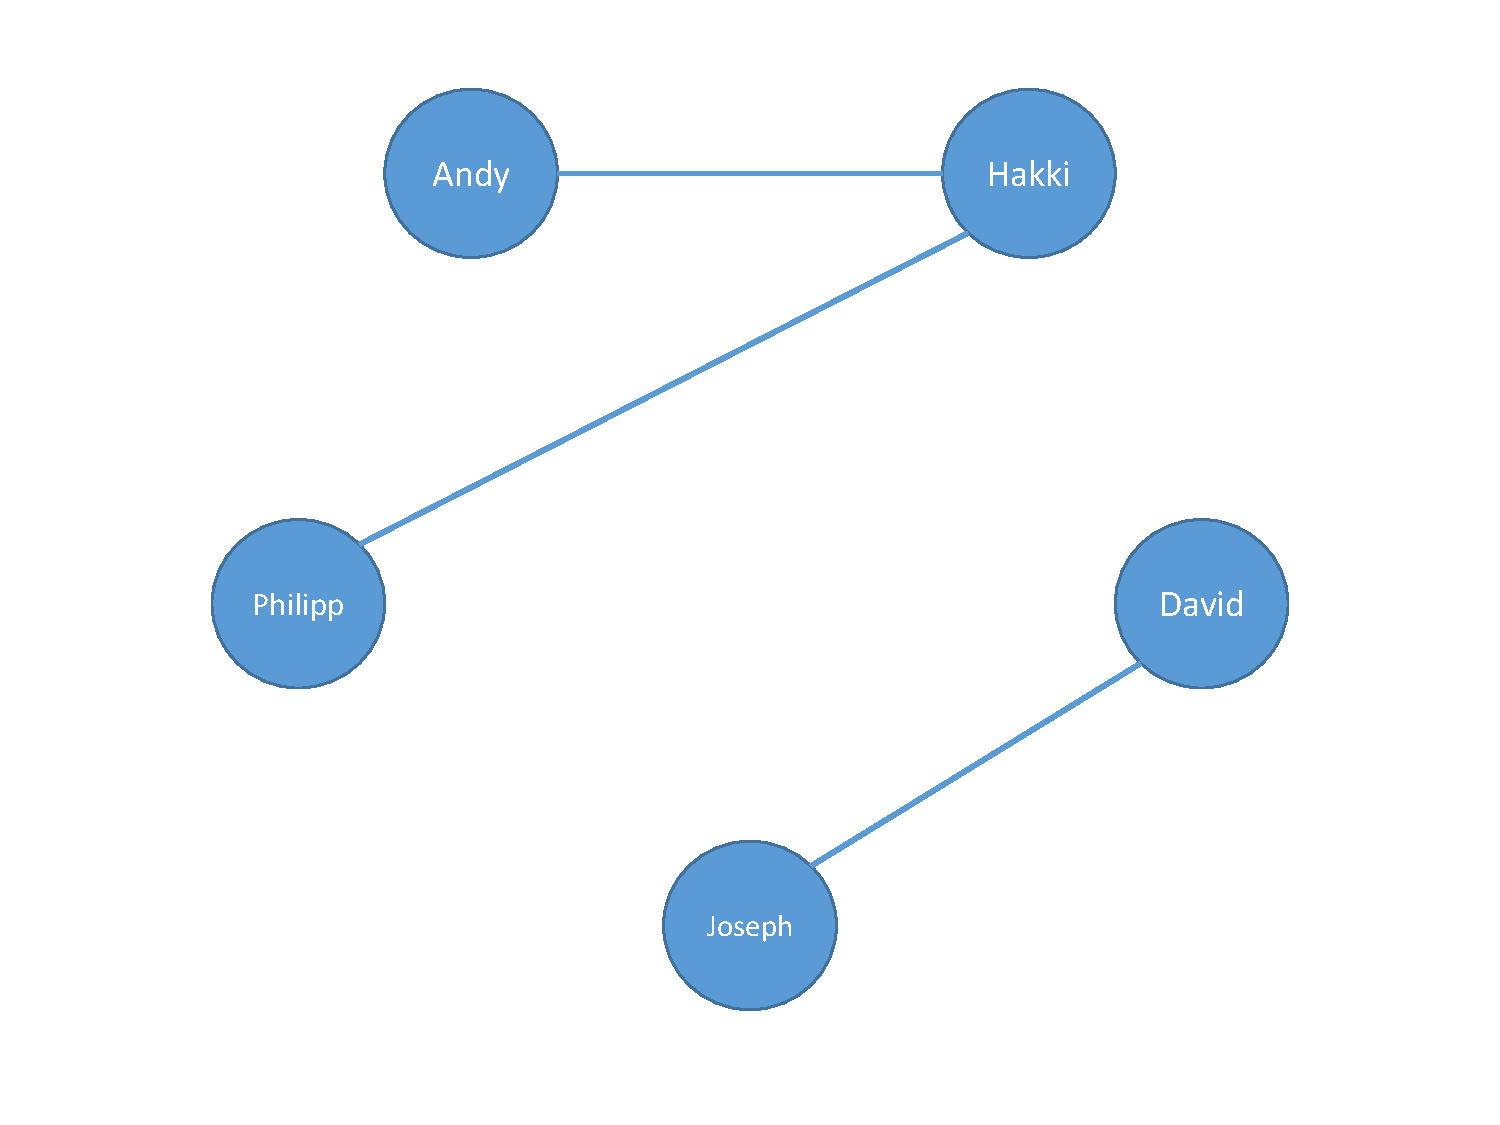
\includegraphics[scale=0.3]{img/foodprefs1.pdf}
}
\only<2>{
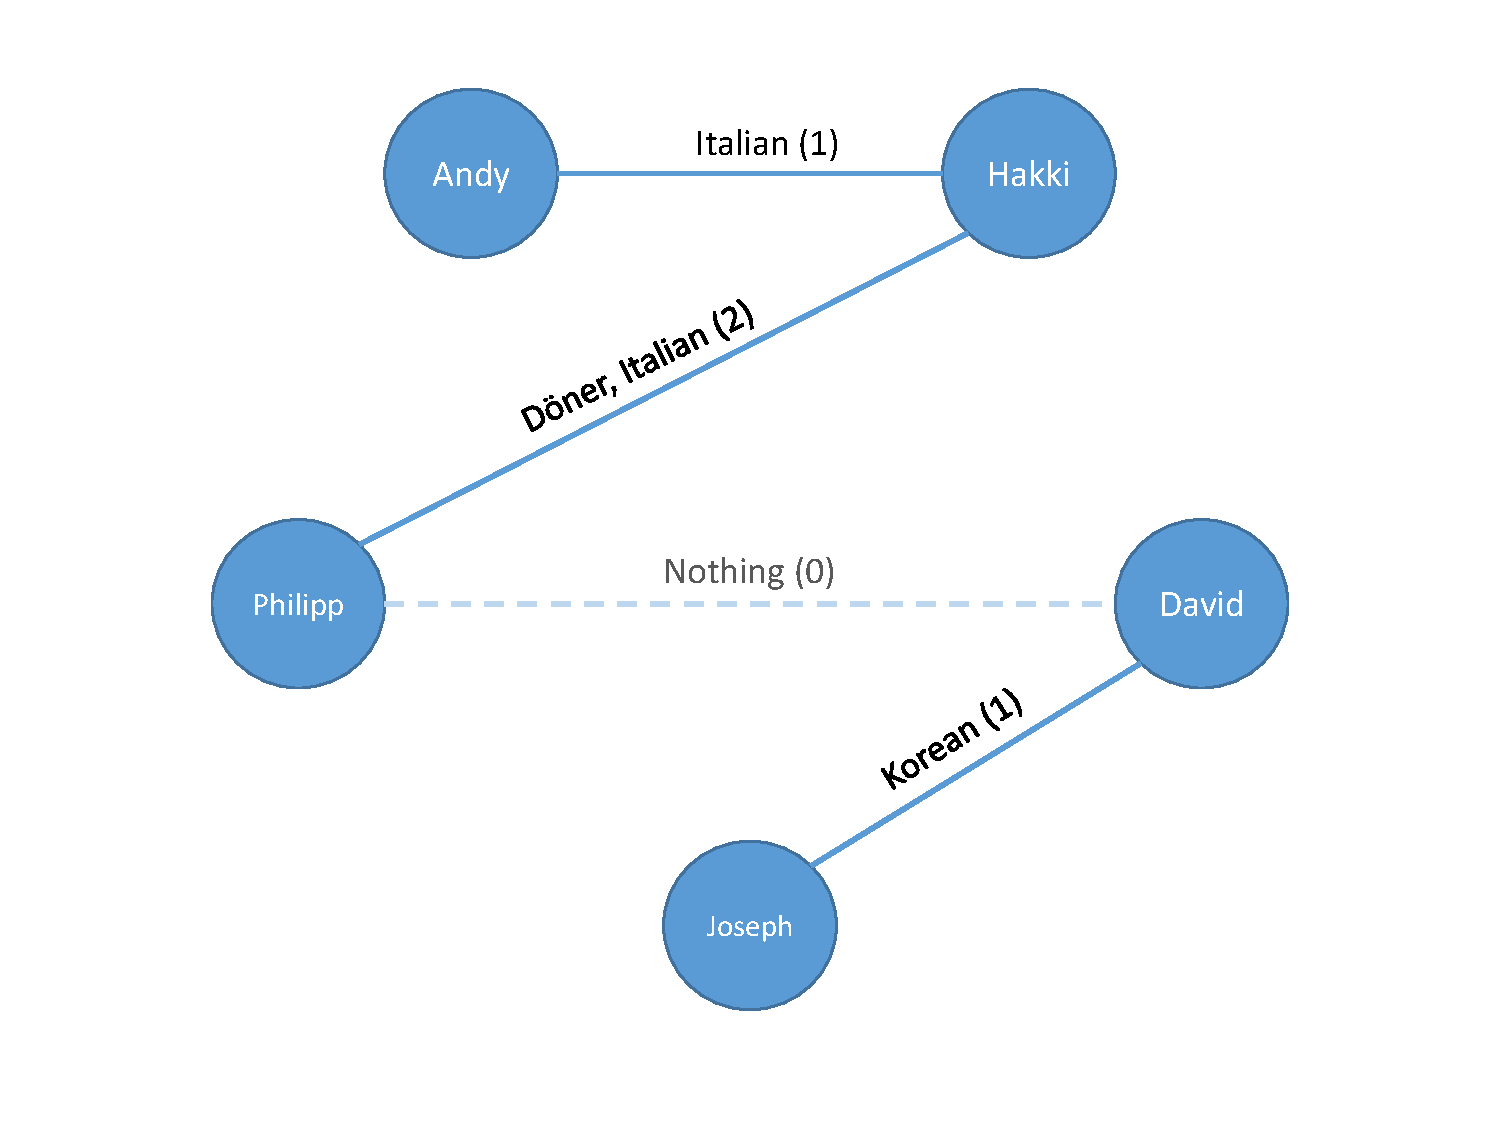
\includegraphics[scale=0.3]{img/foodprefs2.pdf}
}
\only<3>{
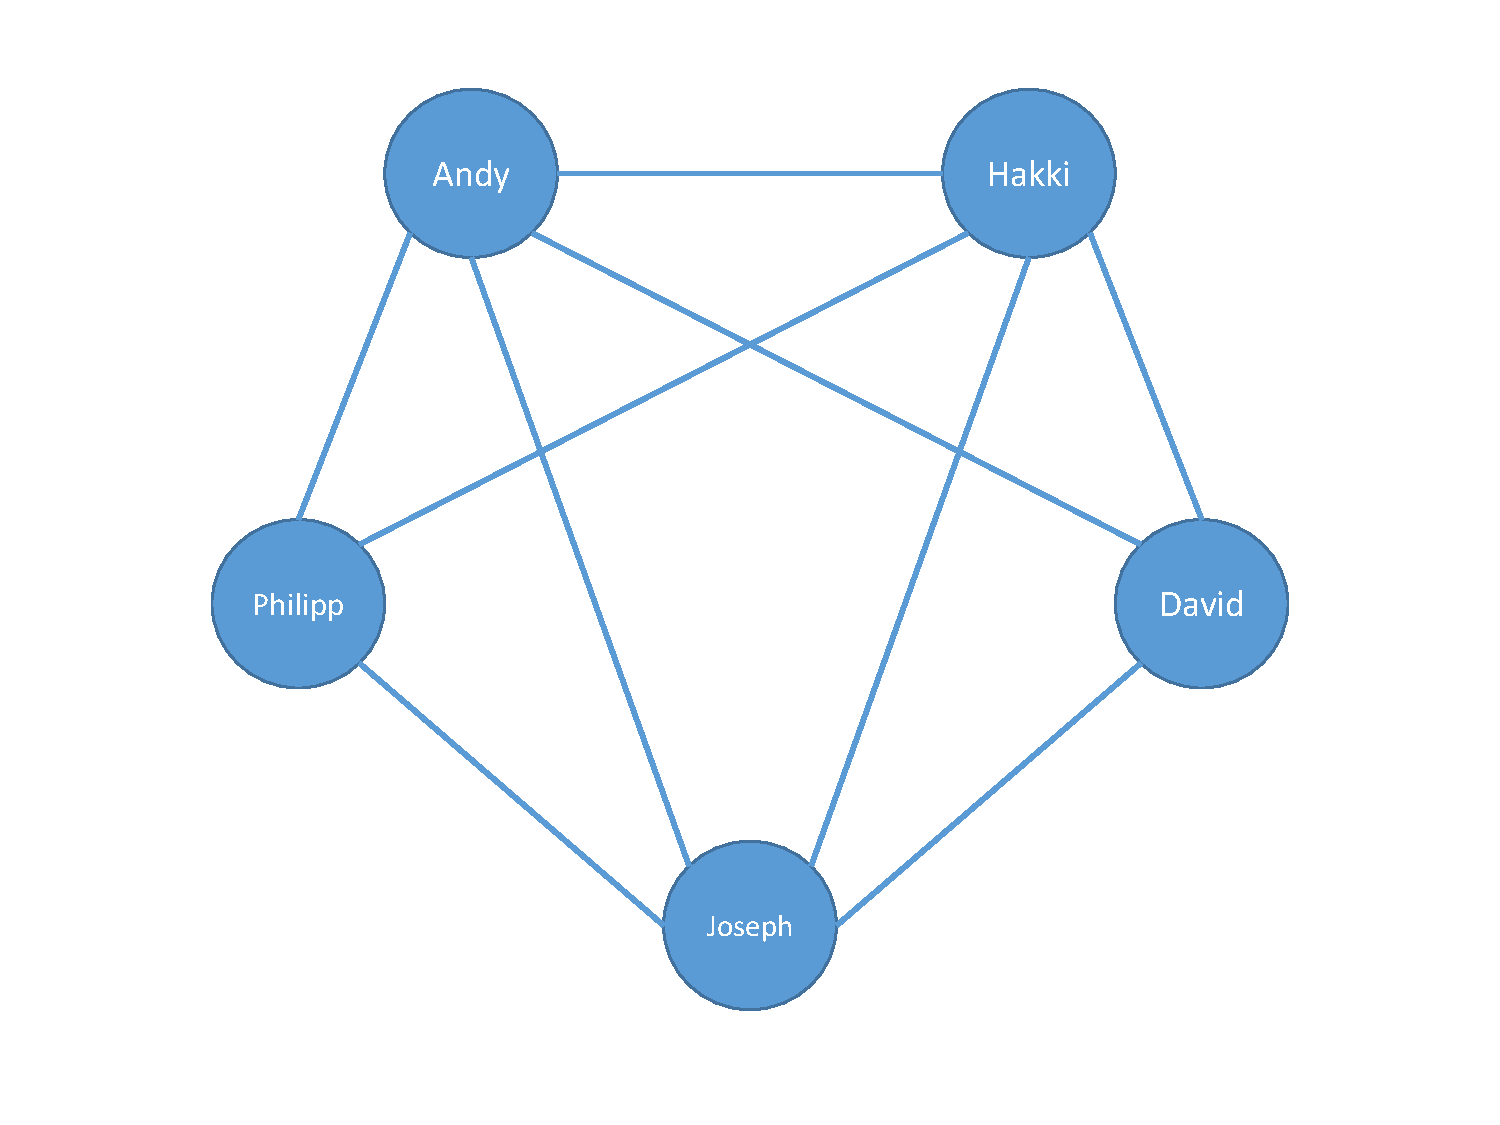
\includegraphics[scale=0.3]{img/foodprefs3.pdf}
}

\end{frame}

\begin{frame}
  \frametitle{Definition}

\only<1>{
  \begin{block}{Cut}
    \begin{itemize}
    \item Undirected graph $G = (V, E)$, $n = \norm{V}$, $m =
      \norm{E}$
    \item Cut problems can be described as partitioning $V$ in to $S$
      and $\overline{S}$, where $S \subset V$:
      \begin{greenblock}{Description}
        \begin{itemize}
        \item Alternatively, finding a subset of $E$ that, if
          removed, splits the graph into two connected componants.
        \item Weight: number of edges between $S$ and $\overline{S}$:
          $$w(S, \overline{S}) = \norm{\{u, v\}\in E ~| ~u \in S \wedge
            v \in \overline{S}}$$
        \end{itemize}
      \end{greenblock}

    \end{itemize}
  \end{block}
}

\only<2>{
  \begin{block}{Min-Cut}
    A cut with minimum weight and $S, \overline{S}
          \ne \phi$

  \end{block}

  \begin{greenblock}{Other Cut Problems}
    \begin{itemize}
    \item Directed Cut: Given $s, t\in V$,ensure $s\in S \wedge t\in
      \overline{S}$;
    \item K-Cut: Cuts the graph into k connected componants;
    \item Sparsest Cut: The sparsest cut problem is to bipartition the vertices so as to minimize the ratio of the number of edges across the cut divided by the number of vertices in the smaller half of the partition.
    \end{itemize}
  \end{greenblock}


}
\end{frame}


\begin{frame}
  \frametitle{Generalization}
  \begin{block}{Difficulty of Cuts}
    Minimum cut can be considered as a subset of $k-cut$ where $k$ is
    a fixed number 2.
    \begin{itemize}
    \item $k-cut$ is $NP-Complete$ problem if $k$ is part of the
      input.
    \item Minimum cut is polynomial time calculable.
    \end{itemize}
  \end{block}

Add anything here?
\end{frame}


\section{Method}
%%% Local Variables:
%%% mode: latex
%%% TeX-master: "../frankfurt"
%%% End:

\subsection{}
\begin{frame}
  \frametitle{Karger's Algorithm}
\only<1>{
      \begin{itemize}
    \item Contraction method is used.
      \item Randomized selection of Edges.
        \item Running multiple times of the algorithm will provide
          more accurate result.
    \end{itemize}
}

\only<2>{
  \begin{itemize}
\item Basically one run of Karger's Algo takes {\bf $O(n^2)$} time;
\item One time running the algorithm will make errors at the
  probability of  $O(\frac{1}{n^2})$;
\item Higher accuracy can be achieved by running the algorithm
  multiple times;
\item It achieves error probability of $\frac{1}{poly(n)}$ with
  $O(n^4\log{}n)$ time.
  \end{itemize}


}
\only<3>{

  \begin{itemize}
  \item Improved Karger's algorithm was developed by Karger and Stein;
  \item Achieving $O(n^2\log^3{n})$ running time;
  \item $O(\frac{1}{n})$ error probability.
  \end{itemize}
Derivation will be given in the later part.
}

\only<4>{

  \begin{block}{Comparison}
    \begin{itemize}
    \item A trivial algorithm checks all x {\bf \large TODO} possible subsets of $V$ and
      computes the weight of the resulting cuts, which takes {\bf
        \large TODO} time in total.
    \item Another algorithm({\bf\large TODO} the one that's based on
      many max-flow-computation) takes {\bf\large TODO} time.
    \end{itemize}
  \end{block}
 Well that's a lot of TODOS
}
\end{frame}


\begin{frame}
  \frametitle{Algorithm}
\only<1>{

\begin{greenblock}{Karger's Algorithm:}
      \begin{algorithm}[H]
        \small
        \Repeat{G has 2 vertices}{
          {\bf choose} an edge $(v, w)$ uniformly at random from G\;
          {\bf let} $G\leftarrow \frac{G}{(v,w)}$
        }
        % \caption{Descent Method Algorithm}
      \end{algorithm}
    \end{greenblock}

}

\only<2>{
\hspace*{1.8cm}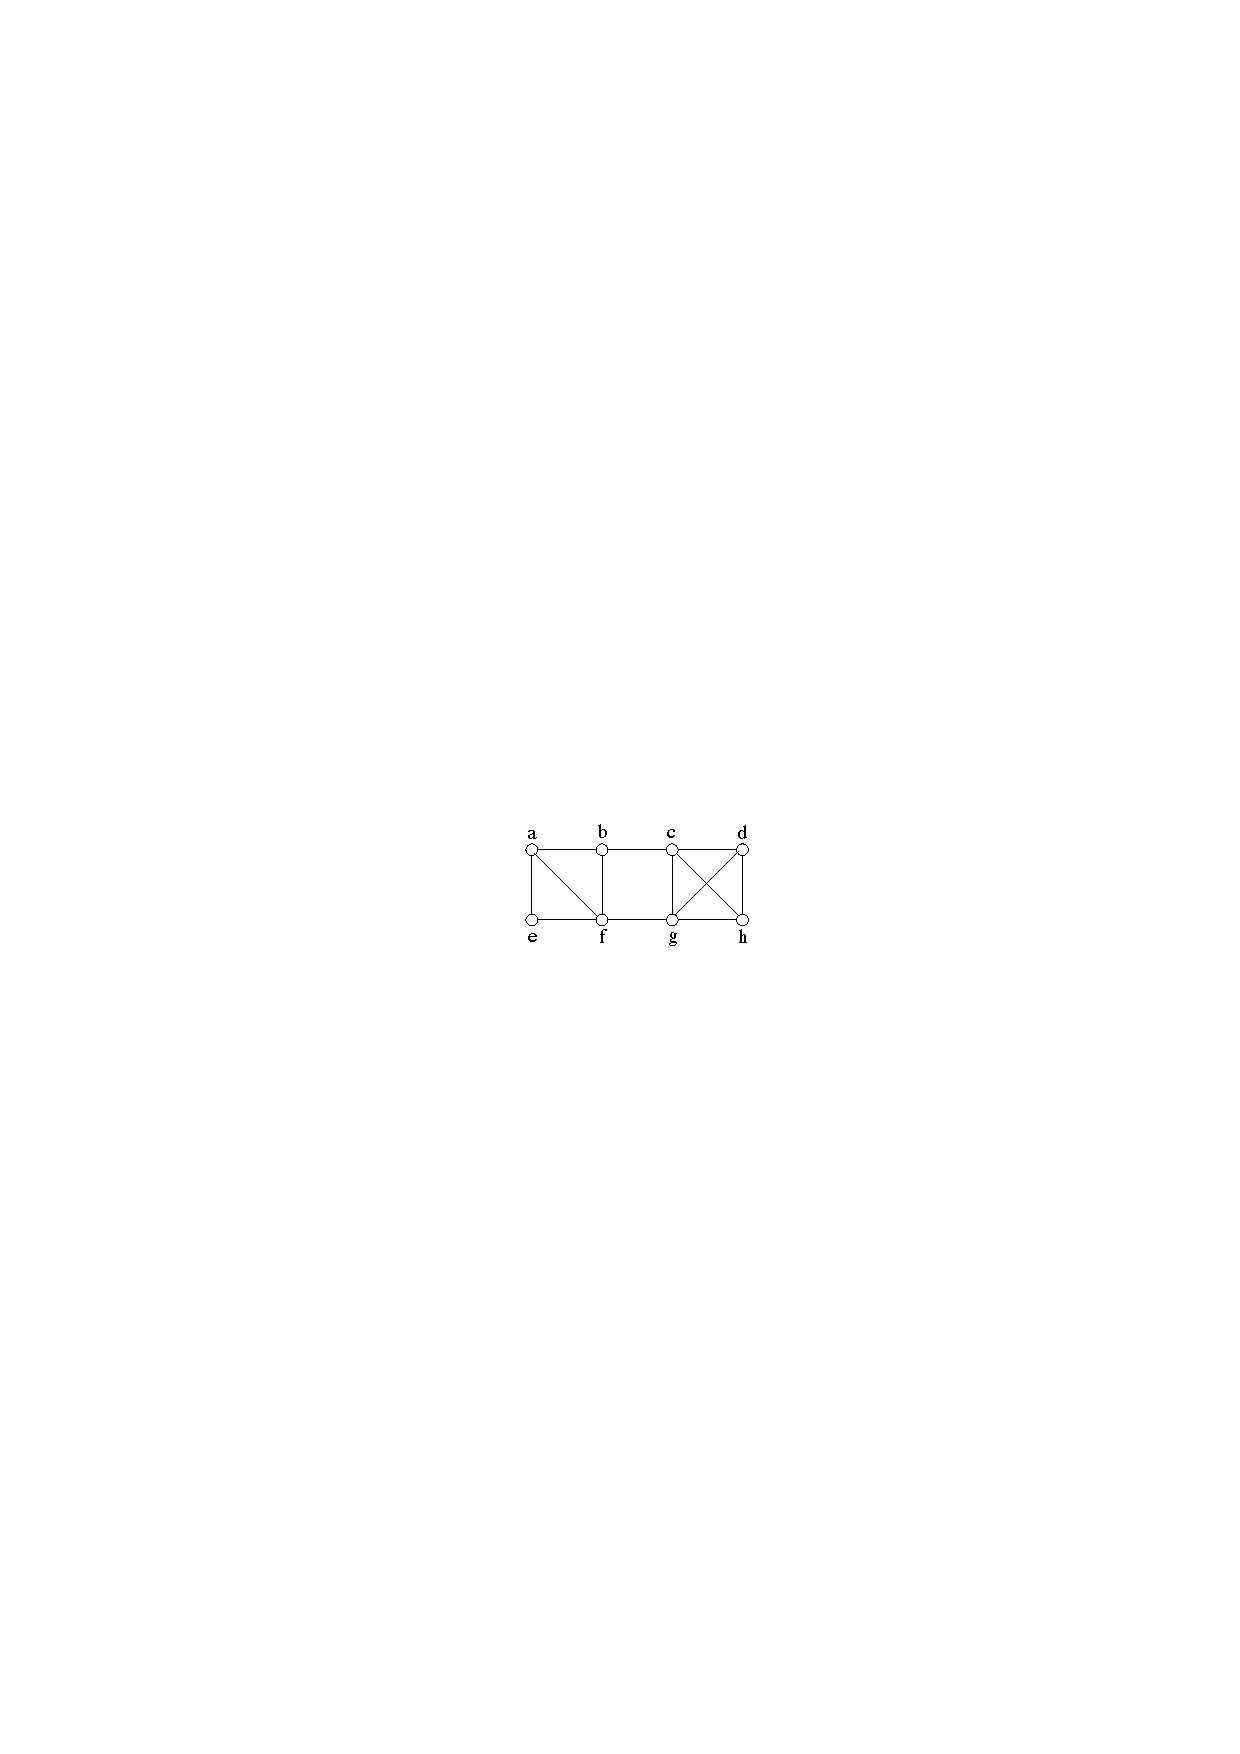
\includegraphics[scale=1.7]{img/examplegraph_modified.pdf}

}
\only<3>{
\hspace*{1.8cm}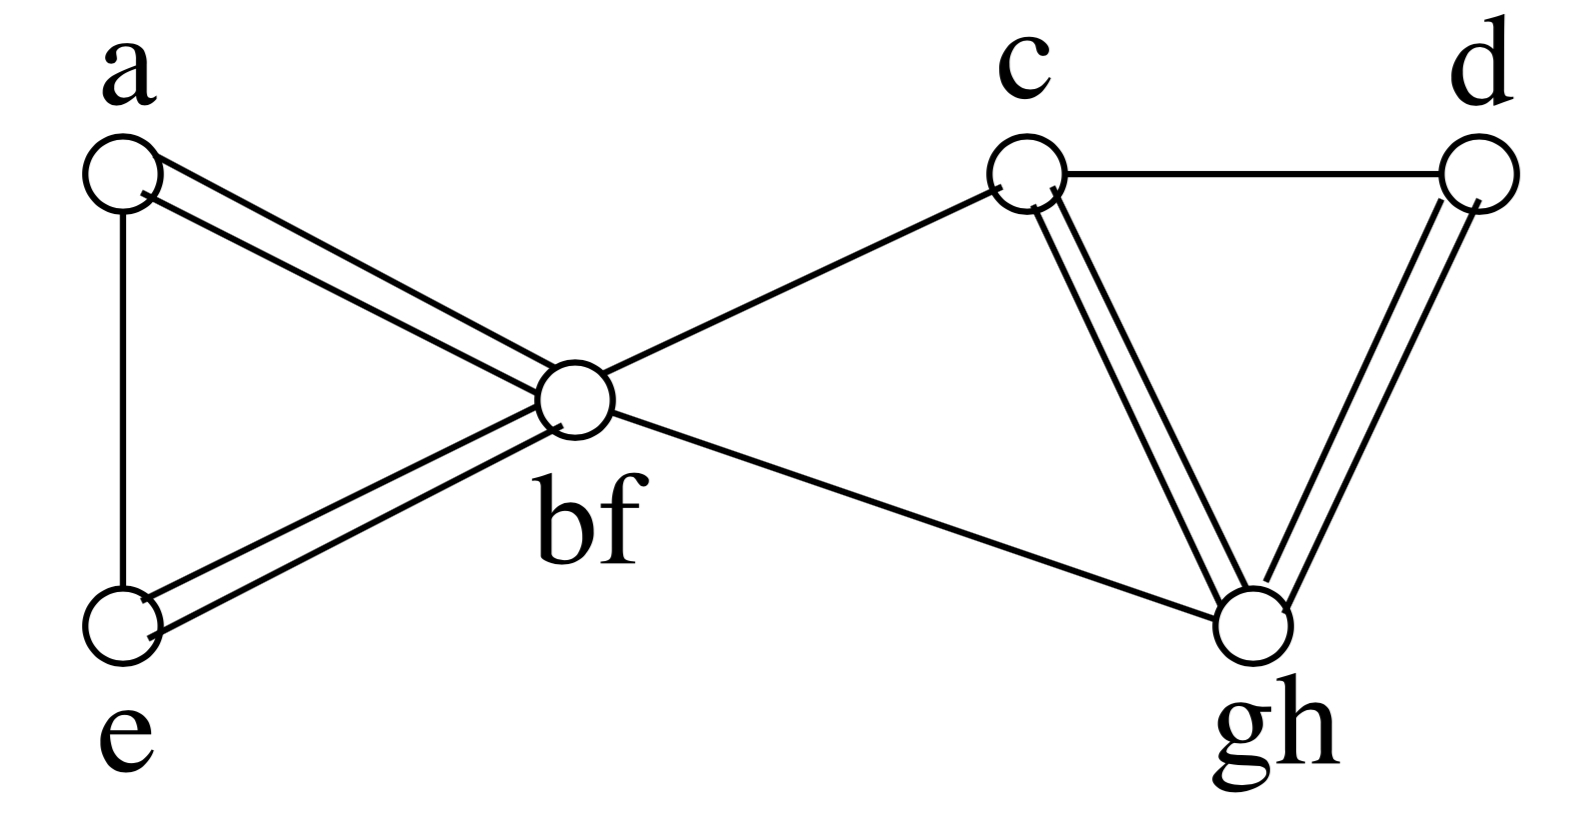
\includegraphics[scale=0.2]{img/2.png}

}
\only<4>{
\hspace*{1.8cm}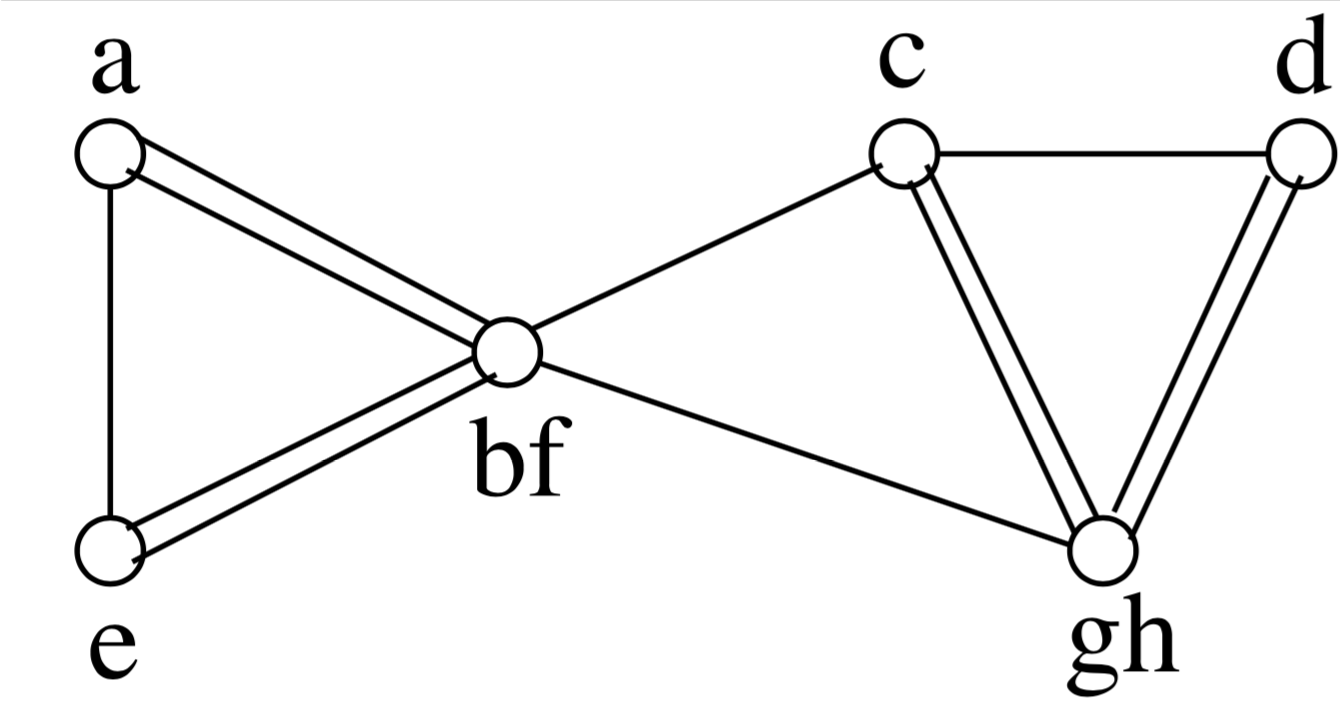
\includegraphics[scale=0.2]{img/3.png}

}
\only<5>{
\hspace*{1.8cm}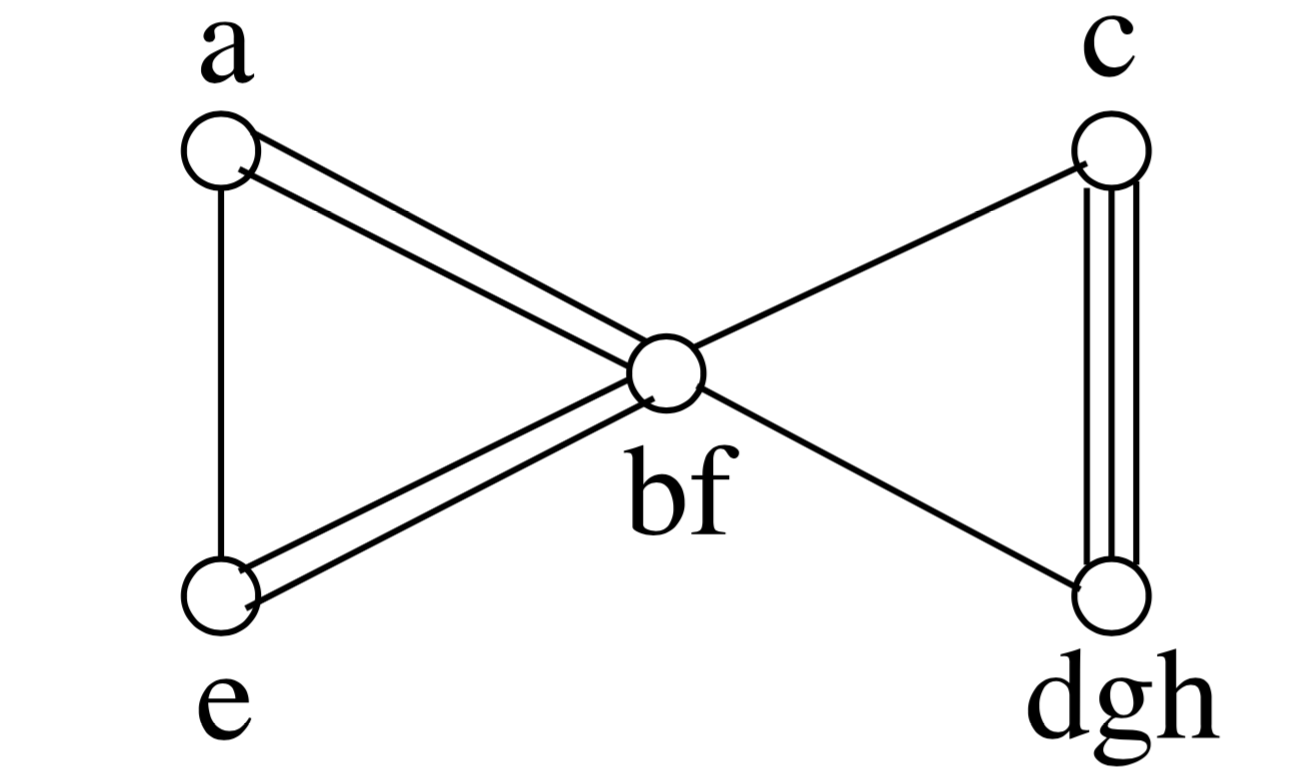
\includegraphics[scale=0.2]{img/4.png}

}
\only<6>{
\hspace*{1.8cm}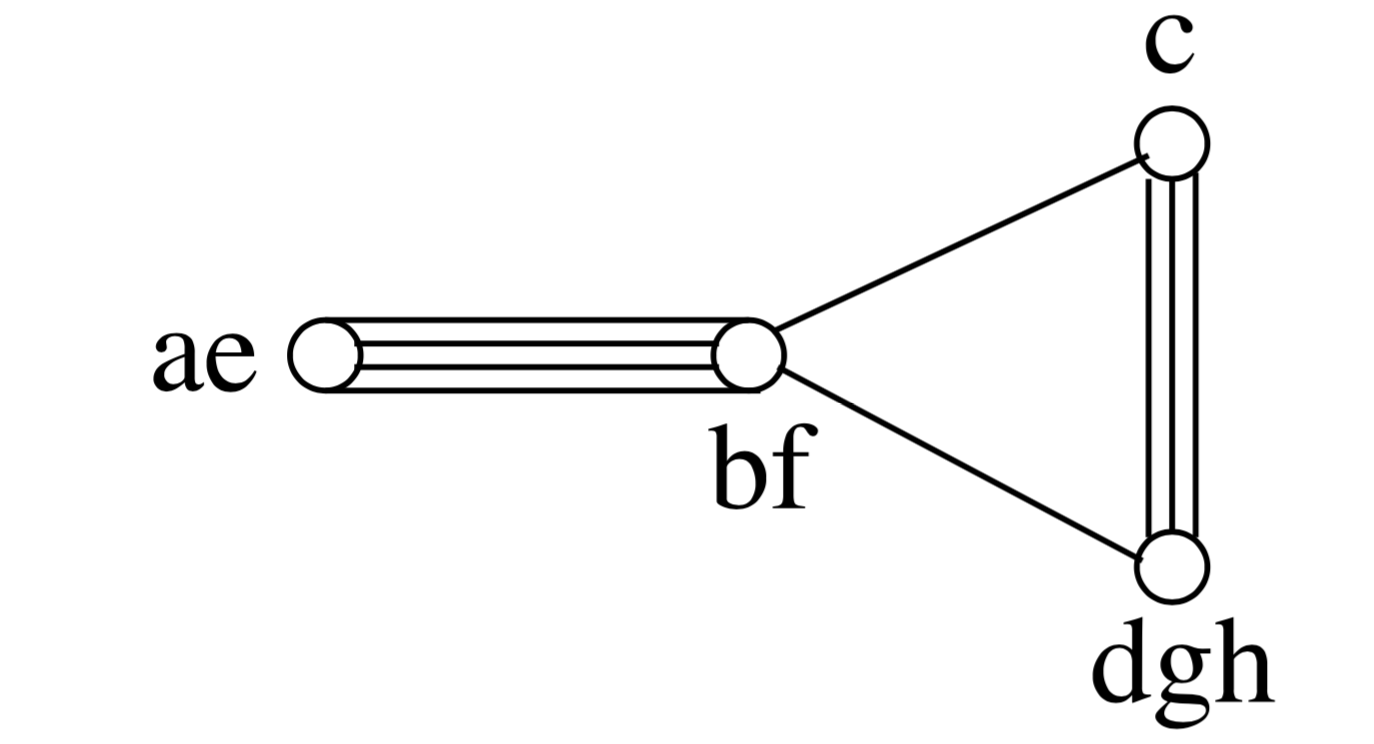
\includegraphics[scale=0.2]{img/5.png}

}
\only<7>{
\hspace*{1.8cm}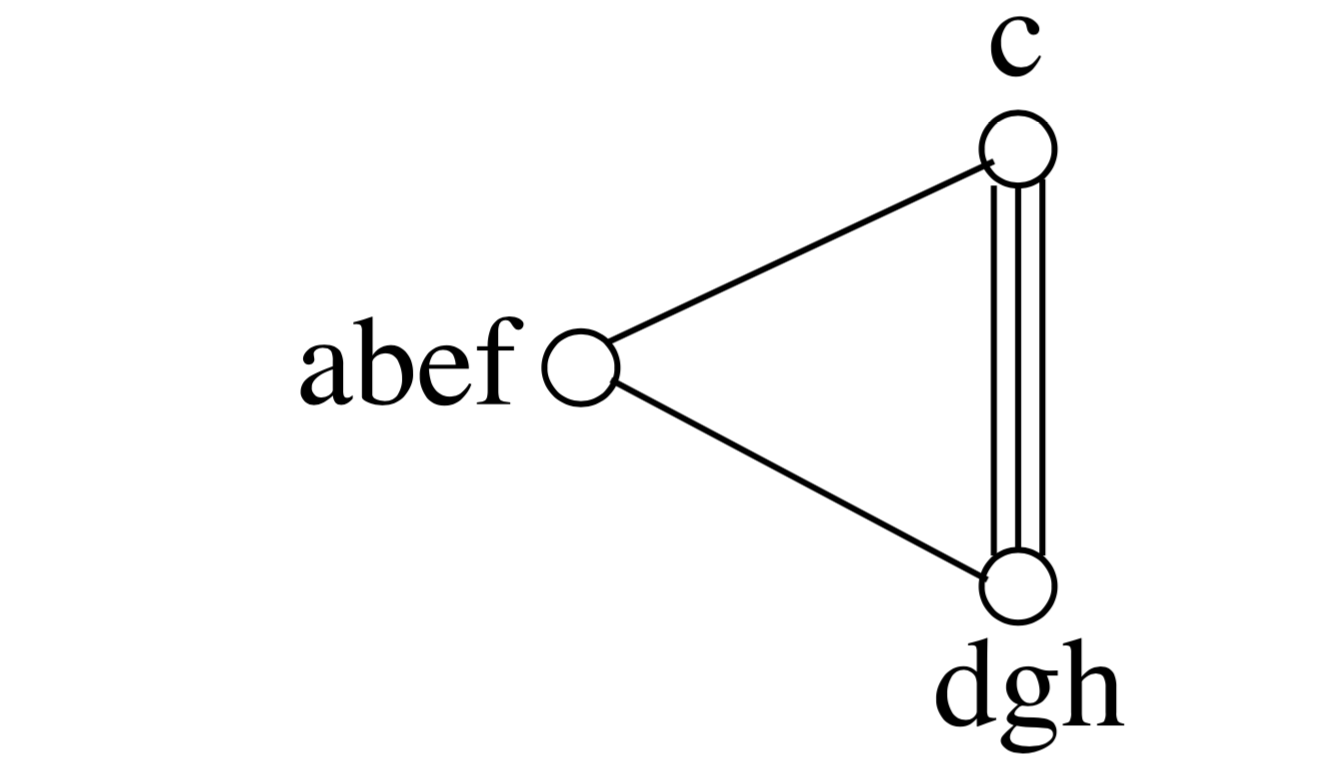
\includegraphics[scale=0.2]{img/6.png}
}

\only<8>{
\hspace*{1.8cm}
\includegraphics[scale=0.2]{img/7.png}
}

% http://www.cs.berkeley.edu/~jordan/courses/174-spring02/recitation/lec5.pdf
\end{frame}

\begin{frame}
  \frametitle{Results}

\vspace*{-1.5cm}
  \hspace*{2cm}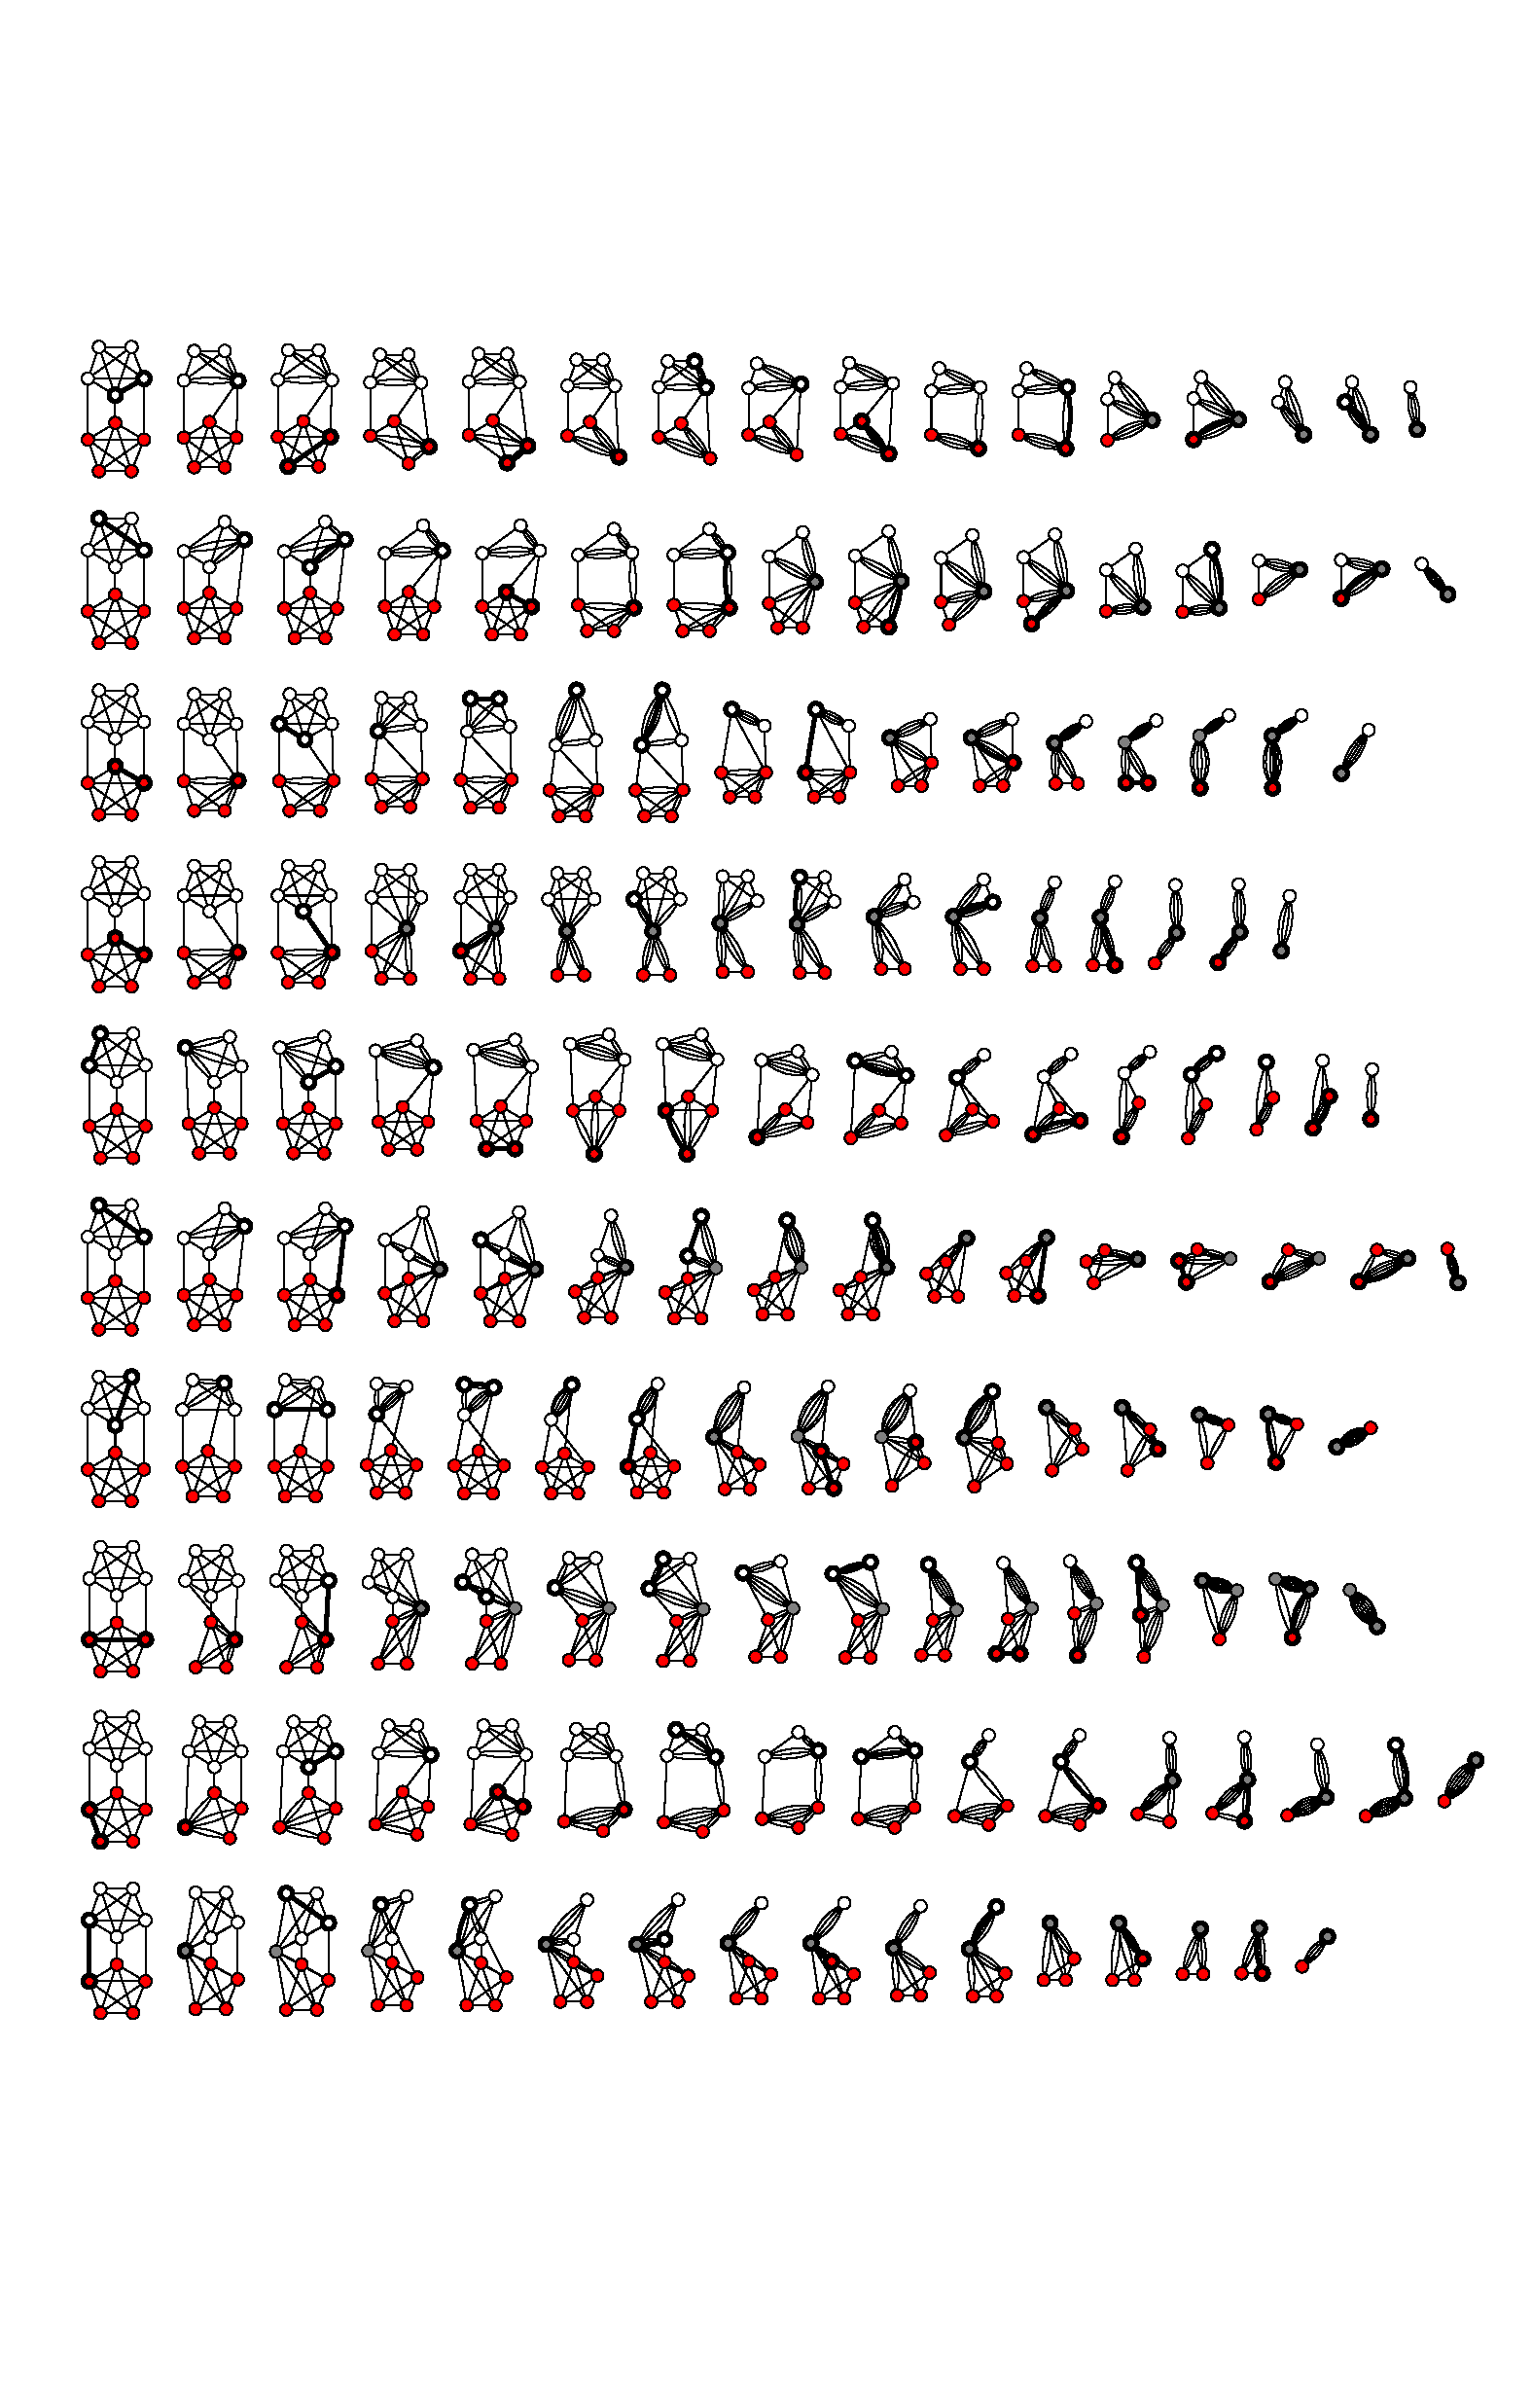
\includegraphics[scale=0.25]{img/kargers.pdf}
\end{frame}


\section{Analysis}
\begin{frame}
  \frametitle{Fact 1 -- Sum of Degrees}
{ \Huge
  \[
    \sum_{u\in V} degree(u) = 2|E|
  \]
}
  Every edge contributes exactly once to the degree of exactly two nodes.
\end{frame}

\begin{frame}
  \frametitle{Fact 2 -- Average Degree}
\begin{equation}
\begin{aligned}
E(degree(X)) & = \sum_{u\in V} Pr(X=u)\cdot degree(u)\\
              & = \frac{1}{n} \sum_u degree(u) = \frac{2|E|}{n}
  \end{aligned}
  \end{equation}
\end{frame}

\begin{frame}
  \frametitle{Fact 3 -- Min-cut Size}

  The size of a min-cut is at most $\frac{2|E|}{n}$.

  \only<1>{ 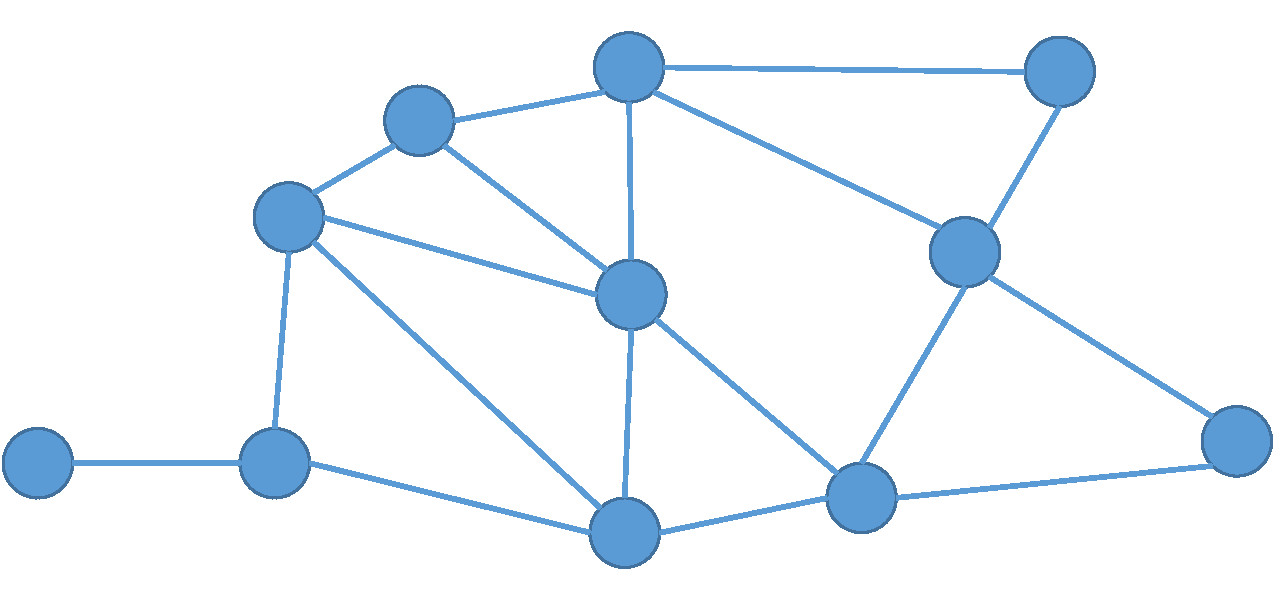
\includegraphics[scale=0.4]{img/fact3_1.pdf} }
  \only<2>{ 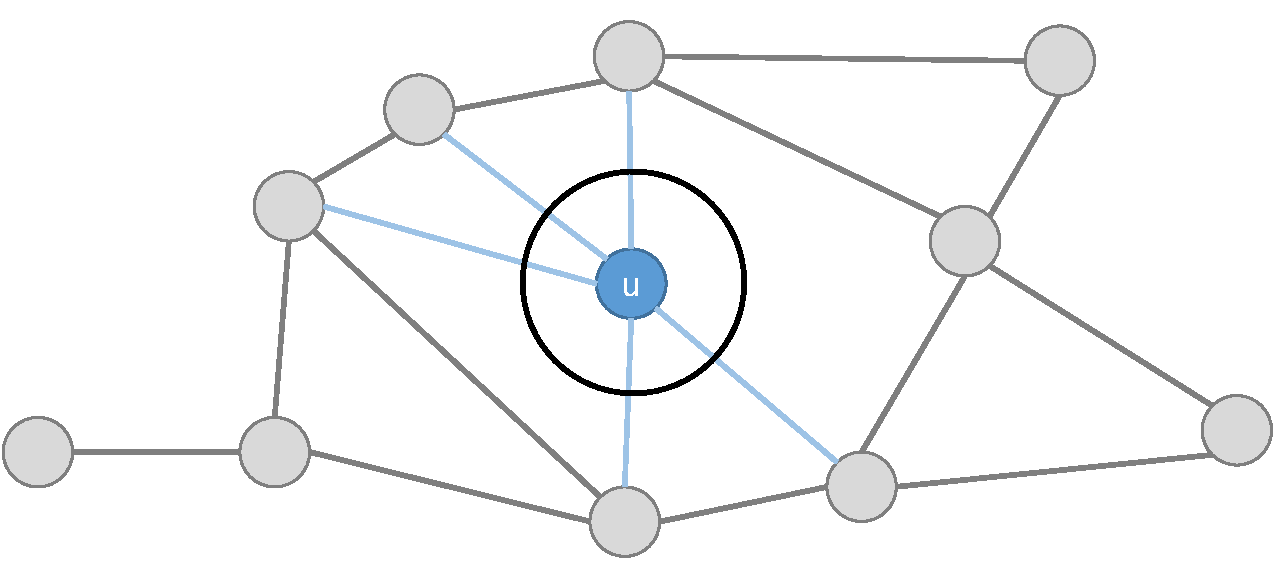
\includegraphics[scale=0.4]{img/fact3_2.pdf} }
  \only<3>{
    \begin{greenblock}{Proof}
      \begin{itemize}
        \item For every node $u$, we have a cut of size $degree(u)$.
        \item Not all nodes can have degree above average, i.e.
      \end{itemize}
      \[
        \exists u\in V:\ degree(u) \leq \frac{2|E|}{n}
      \]
    \end{greenblock}
  }

\end{frame}

\begin{frame}
  \frametitle{Fact 4 -- Pr[edge across min-cut]}

  \begin{itemize}
    \item Fix a certain min-cut in a graph.
    \item At most $2|E|/n$ of all edges are part of this min-cut.
    \item Choose a random edge out of all $|E|$ edges.
    \item $Pr(\text{edge crosses the cut}) = \frac{2|E|/n}{|E|} = \frac{2}{n}$
  \end{itemize}

\end{frame}


\begin{frame}
  \frametitle{Concentrating = Not Cutting}
  \begin{itemize}
  \item {\bf\large TODO} show the running example and explain how an
    edge that has been concentrated will never be cut.
  \item And the edges that remain at the end, because they have never
    been concentrated.
  \end{itemize}
\end{frame}

\begin{frame}
  \frametitle{Success Probability}

\only<1>{
  \begin{itemize}
  \item Fix a certain min-cut
  \item We can never contract an edge from that cut
  \item $Pr[first edge is not in min cut] = 1 - \frac{2}{n}$
  \item Now $n - 1$ edges remaining, so $Pr[second edge is not in min
    cut] = (1 - \frac{2}{n-1})$
  \end{itemize}
}

\only<2>{
  \begin{block}{First Cut is not Fixed Cut }
 \begin{equation*}
    \begin{aligned}
Pr[fi&\left(nal cut is not the fixed cut]\right)\\
   =  &\left(    Pr[no contracted edge is in minimun cut] \right)\\
 \le  & \left(   (1 - \frac{2}{n})(1 - \frac{2}{n-1})(1 - \frac{2}{n-2})...(1 -
   \frac{2}{4})(1 - \frac{2}{3}) \right)\\
  =  &\left(  \frac{n-2}{n} \right)
    \end{aligned}
   \end{equation*}

  \end{block}
}

\only<3>{
  \begin{block}{Series Convere to e}
    \begin{itemize}
    \item $e = \lim(1 + \frac{1}{n})^n$
    \item $\lim(1 + \frac{1}{n})^n = \lim(1 +
      \frac{1}{\frac{n}{a}})^{\frac{n}{a}\cdot a}$
    \item Let $x = \frac{n}{a}$
    \end{itemize}
    $\lim(1 + \frac{1}{n})^n = \lim(1 + \frac{1}{x})^{x\cdot a}$
    $ =( \lim(1 + \frac{1}{x})^x)^a = e^x$
  \end{block}
}

\end{frame}

\begin{frame}
  \frametitle{Boosting Success Probability}

\only<1>{




Assumn that we can get the best result by running the algorithm $k$
times.
\begin{itemize}
\item Probability of at least one success:
$1 - (1 - \frac{1}{\binom{n}{2}})^k$
\item To make it an e-series, we need $k$ to contain $\binom{n}{2}$.
\end{itemize}

Here we can use $a = -1$ and $k = \binom{n}{2}\cdot c\cdot \ln{n}$
Running time is thus promised:
$$O(k)\cdot O(n^2) = O(n^4\log{n})$$

}

\only<2>{
  \begin{equation*}
    \begin{aligned}
1 - (1 - \frac{1}{\binom{n}{2}})^k  &= 1 - (1 +
\frac{1}{\binom{n}{2}})^{-k}\\
& =1 - ((1 + \frac{1}{\binom{n}{2}})^{\binom{n}{2}})^{-c\cdot\ln{n}}\\
& = 1 - e^{-c\cdot\ln{n}} = 1 - (e^{\ln{n}})^{-c}\\
& =1 - \frac{1}{n^c}
    \end{aligned}
  \end{equation*}


}

\only<3>{
The error probability is thus:

$$
O( \frac{1}{n^c})
$$

}
\end{frame}


\begin{frame}
  \frametitle{Extended Karger's Analysis}
One run succeeds with $\Omega(\frac{1}{\log{n}})$. If we run the
algorithm$k = \log^2{n}$ times:
\begin{equation*}
  \begin{aligned}
Pr[at least one run succeeds] & =1 - (1 - \frac{1}{log{n}})^{\log^2{n}}\\
& = 1 - (1 + \frac{1}{-log{n}})^{-\log{n}\cdot-\log{n}}\\
& =1 -e^{-\log{n}} = 1 - \frac{1}{n}
& \Rightarrow Error Probability O(\frac{1}{n})
  \end{aligned}
\end{equation*}
\end{frame}



% \begin{frame}
%   % \frametitle{Table of contents}
%   % \tableofcontents
% %%% Local Variables:
%%% mode: latex
%%% TeX-master: t
%%% End:

%%  commands definition and some other definitions about stuffs
\newcommand\here{lalala}
%\newcommand\x{x_i}
%\newcommand\y{y_i
\newcommand\dis{\displaystyle }


\subsection{}
\begin{frame}
  \frametitle{Linear Regression Example}
  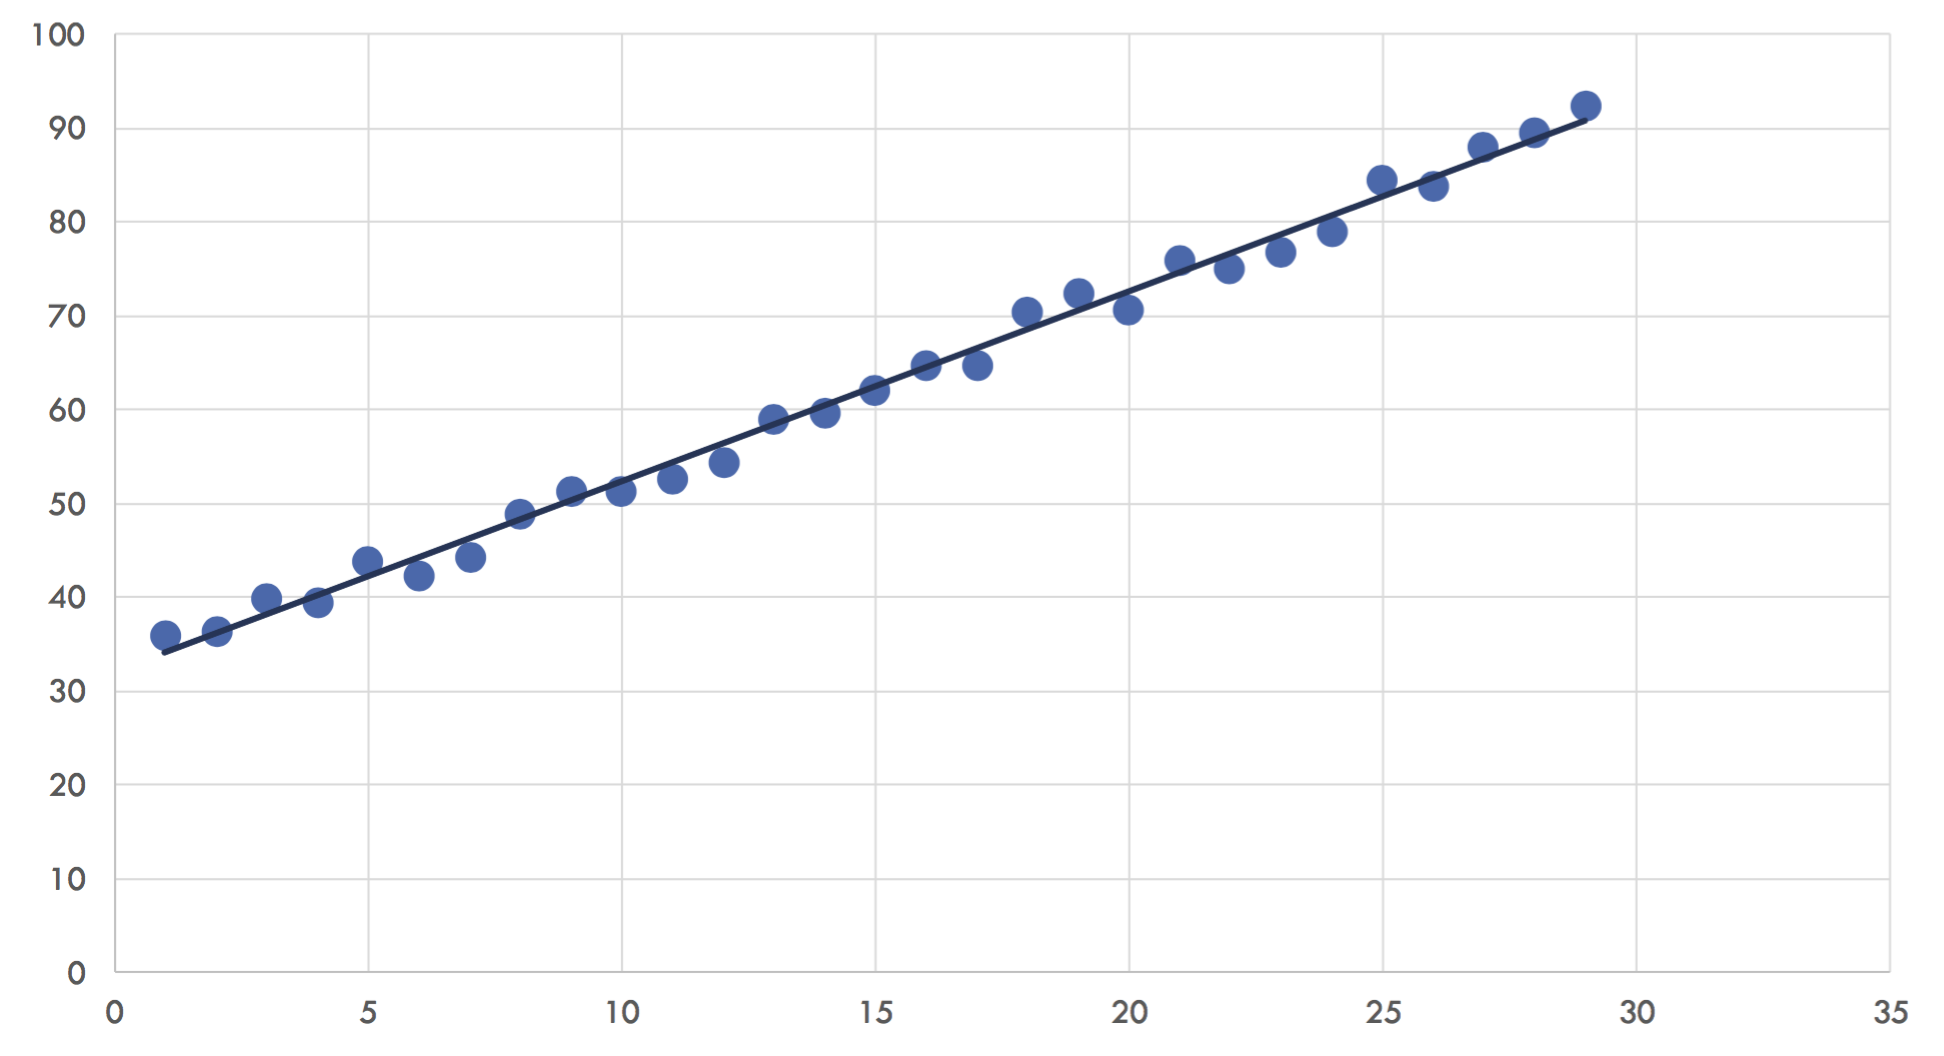
\includegraphics[scale=0.32]{pics/linear.png}

\end{frame}


\subsection{}
\begin{frame}
\frametitle{Ordinary Least Squares}

% 2 columns examples
\begin{columns}
  \begin{column}{0.6\textwidth}
    \begin{itemize}
    \item[] Input: points $(x_i, y_i)$
      \item[] Regression line: $y = mx + b$
\item[] Objective: $\displaystyle \min_{m, b} \sum_{i}(y_i - mx_i -b)^2$
    \end{itemize}
  \end{column}

  \begin{column}{0.5\textwidth}
    \begin{itemize}
    \item[] $(\vec{x_i}, y_i)$
    \item[] $y = \vec{w} \cdot \vec{x} + b$
    \item[] $\dis \min_{\vec{w}}\sum_{i}(y_i - \vec{w} \cdot \vec{x_i} -b)^2$
    \end{itemize}

  \end{column}
\end{columns}

\begin{itemize}
\item Easily Solved: $\vec{w}^*(X^TX)-X^T\vec{y}$
\item But what if $\dim\vec{x} $ is large?
\item What about other similar regressions?
\end{itemize}

\end{frame}

\subsection{}
\begin{frame}
\frametitle{Convex Optimization Problems}


\begin{itemize}
\item OrdinaryLinearRegression: $\dis \min_{\vec{w}}\sum_i(y_i -
  \vec{w} \cdot \vec{x_i})^2$
\item General: $\dis \min_xf(x)$ where $f(x)$ is convex
\item Set $C$ is convex $\Longleftrightarrow \forall x, y\in C, 0\le t
  \le 1: tx +(1 - t)y \in C$
\item Function $f : \mathbb{R}^n \rightarrow \mathbb{R}$ is convex if
  $\dom f$ is convex and $\exists x, y \in \dom f, 0\le t \le 1:$

\end{itemize}

\vspace{-4mm}

{\small
$$f(tx + (1 - t)y) \le tf(x) + (1 - t)f(y)$$
}

\vspace{-4mm}

\begin{columns}
  \begin{column}{0.5\textwidth}

\begin{itemize}
\item Unconstrained.
\end{itemize}

  \end{column}

  \begin{column}{0.5\textwidth}
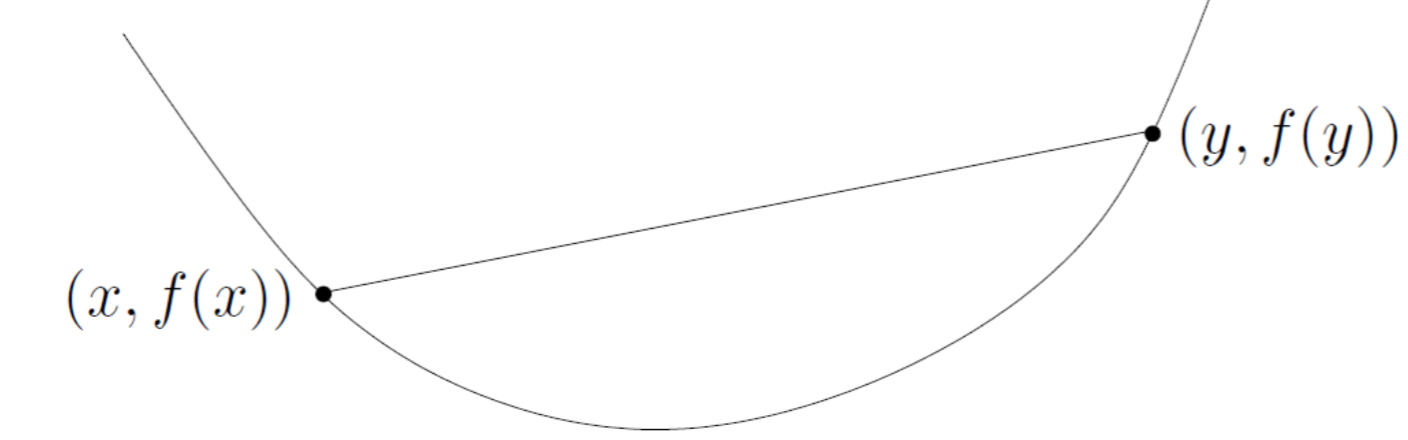
\includegraphics[scale=0.2]{pics/uncons.png}
  \end{column}
\end{columns}

\end{frame}

\subsection{}

\begin{frame}
  \frametitle{Outliers}
  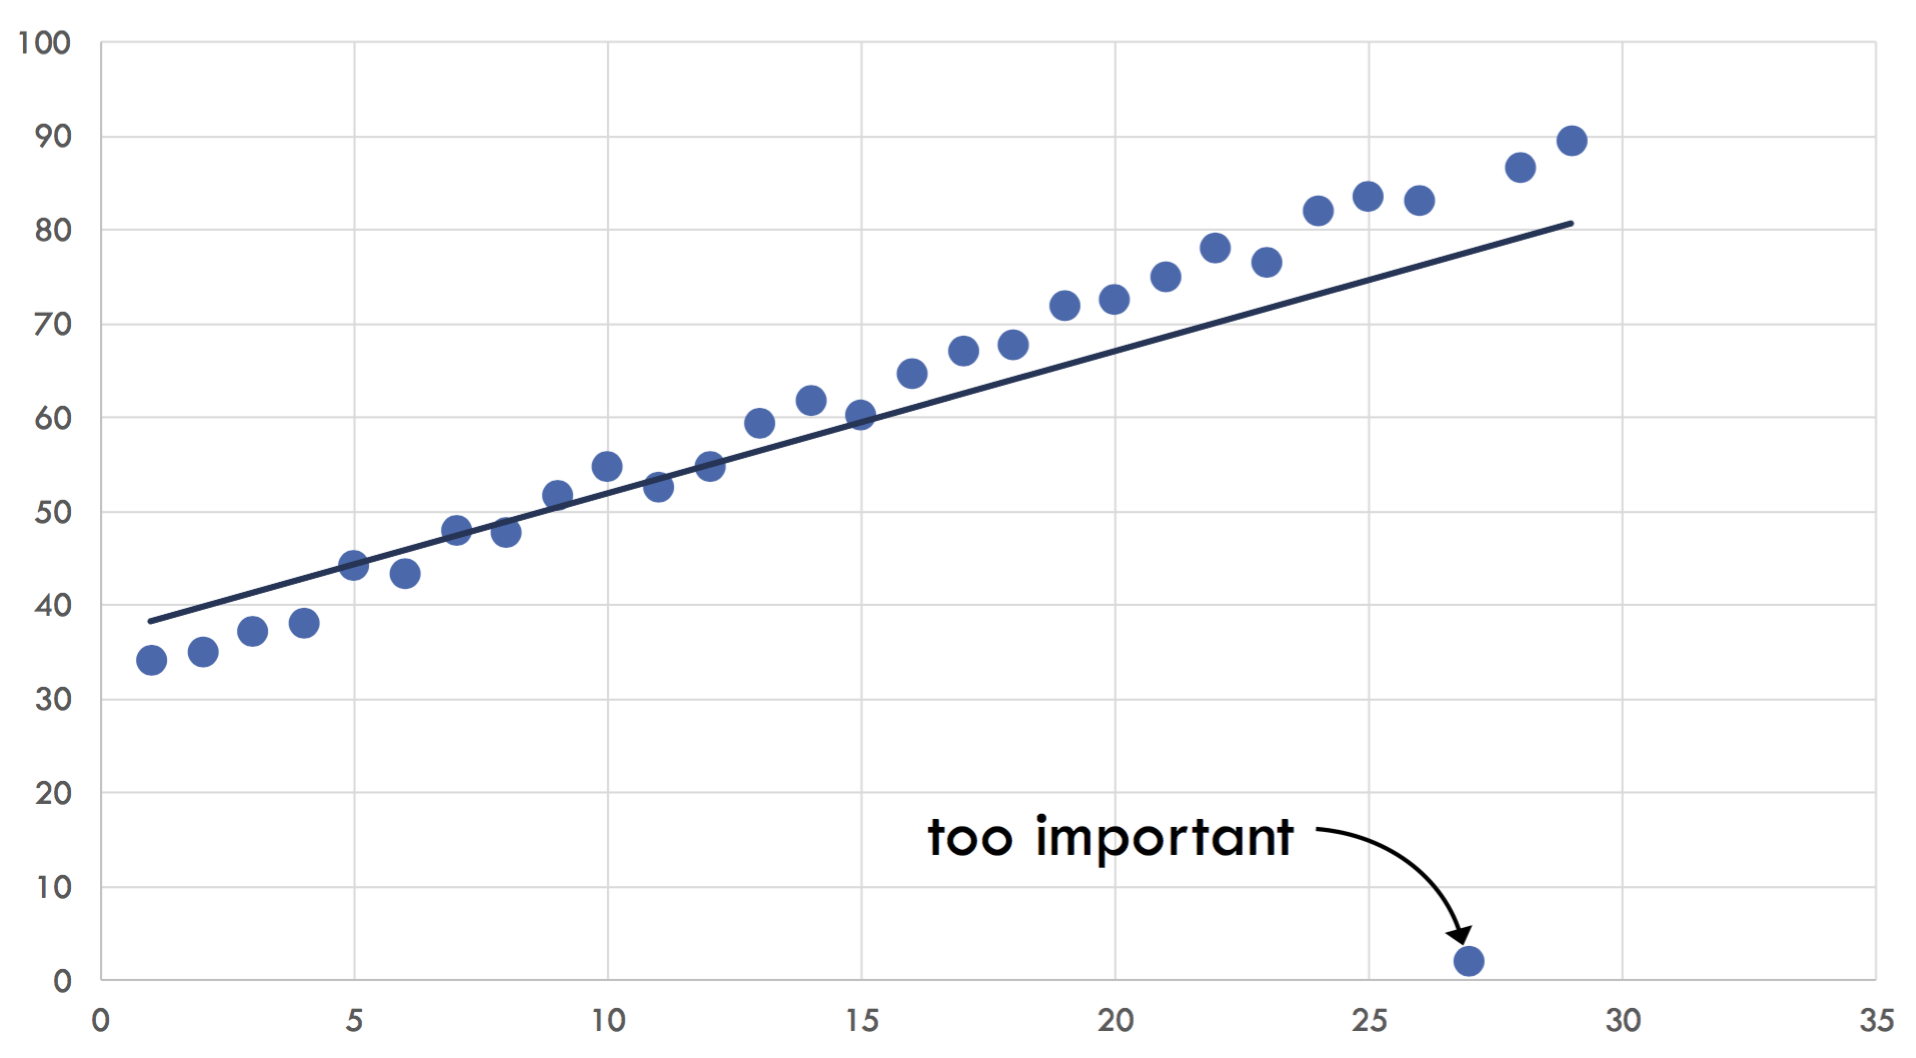
\includegraphics[scale=0.32]{pics/lpo.png}

\end{frame}

\subsection{}
\begin{frame}


  \frametitle{Outlier Penalty}

  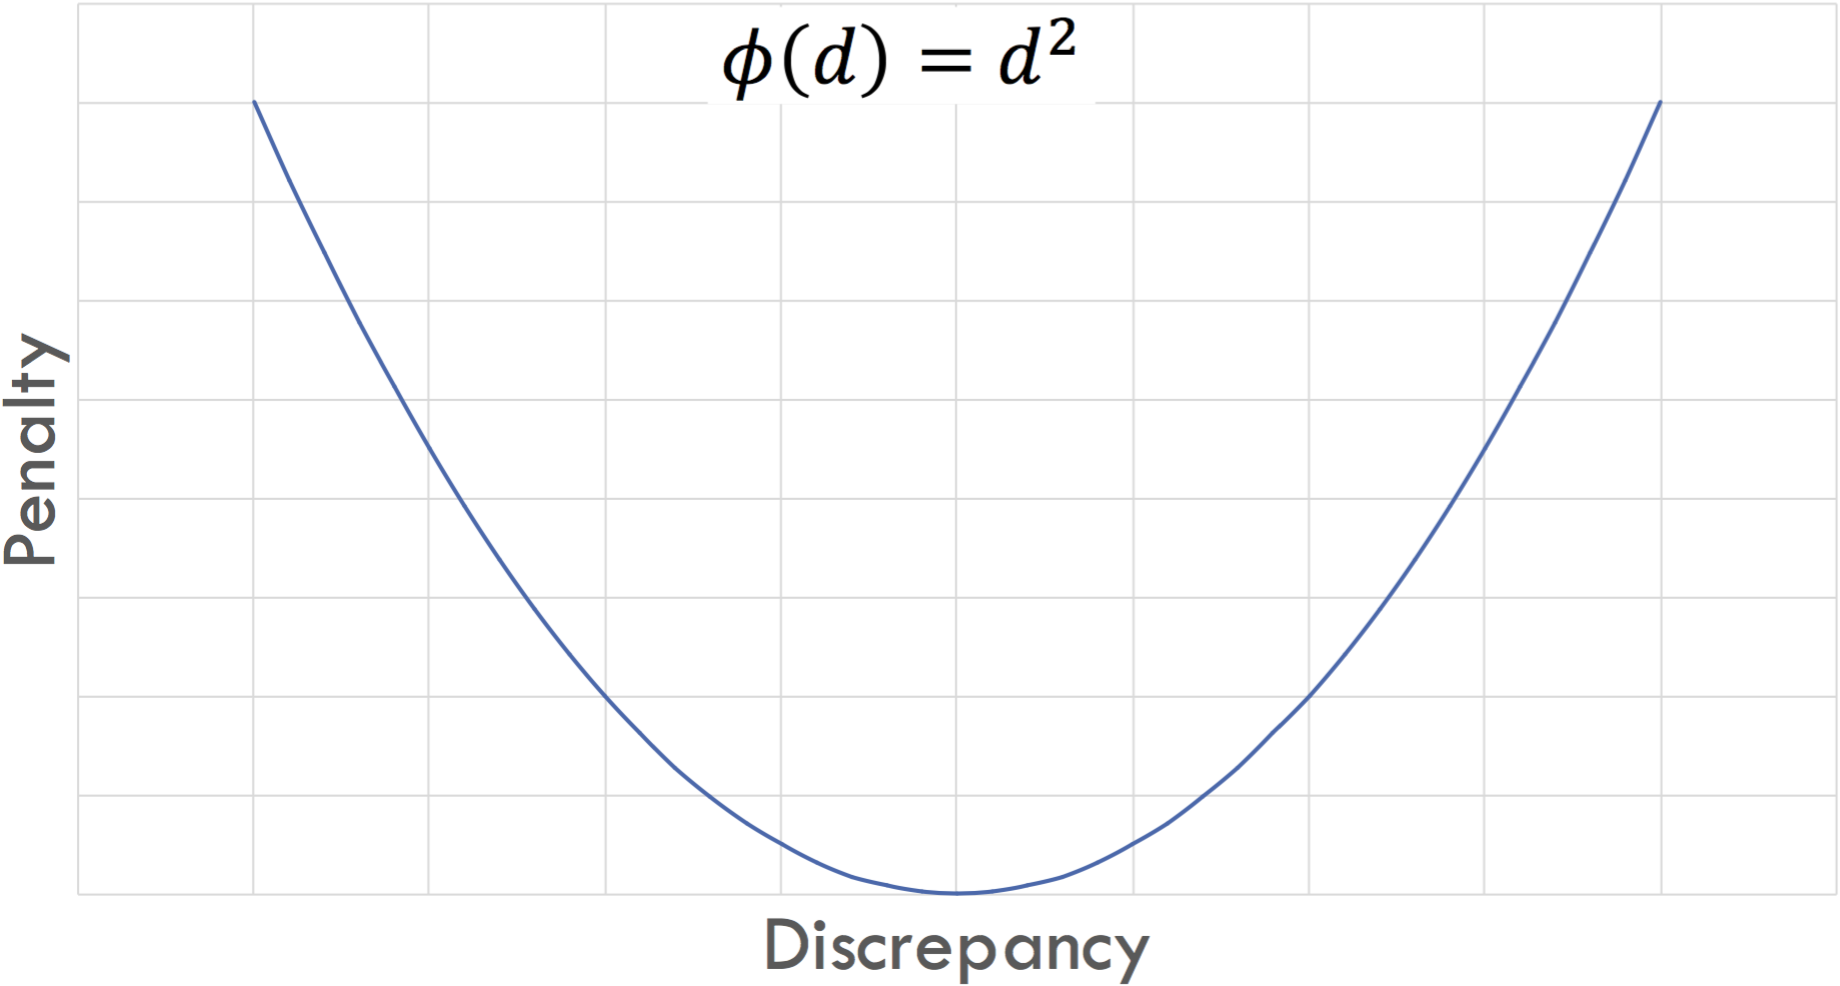
\includegraphics[scale=0.32]{pics/pen1.png}


\end{frame}

\begin{frame}
  \frametitle{Capped Penalty}
  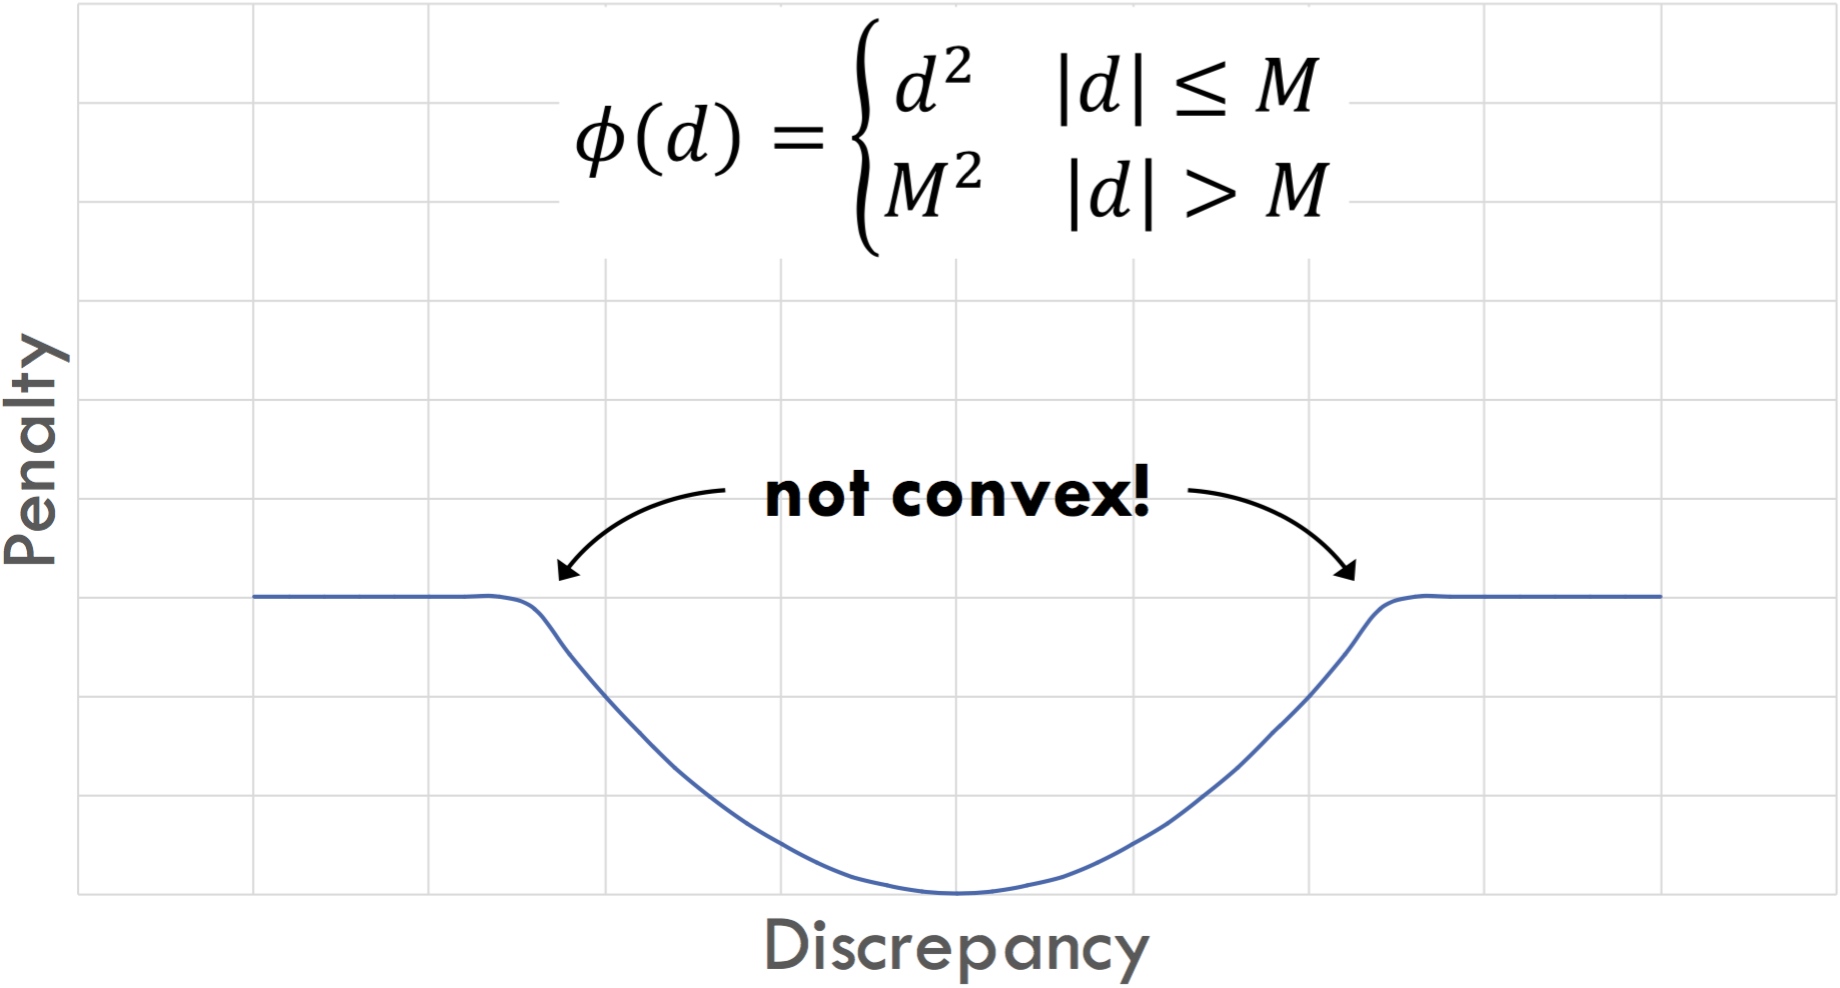
\includegraphics[scale=0.32]{pics/pen2.png}
\end{frame}

\begin{frame}
\frametitle{Huber Penalty Function}
  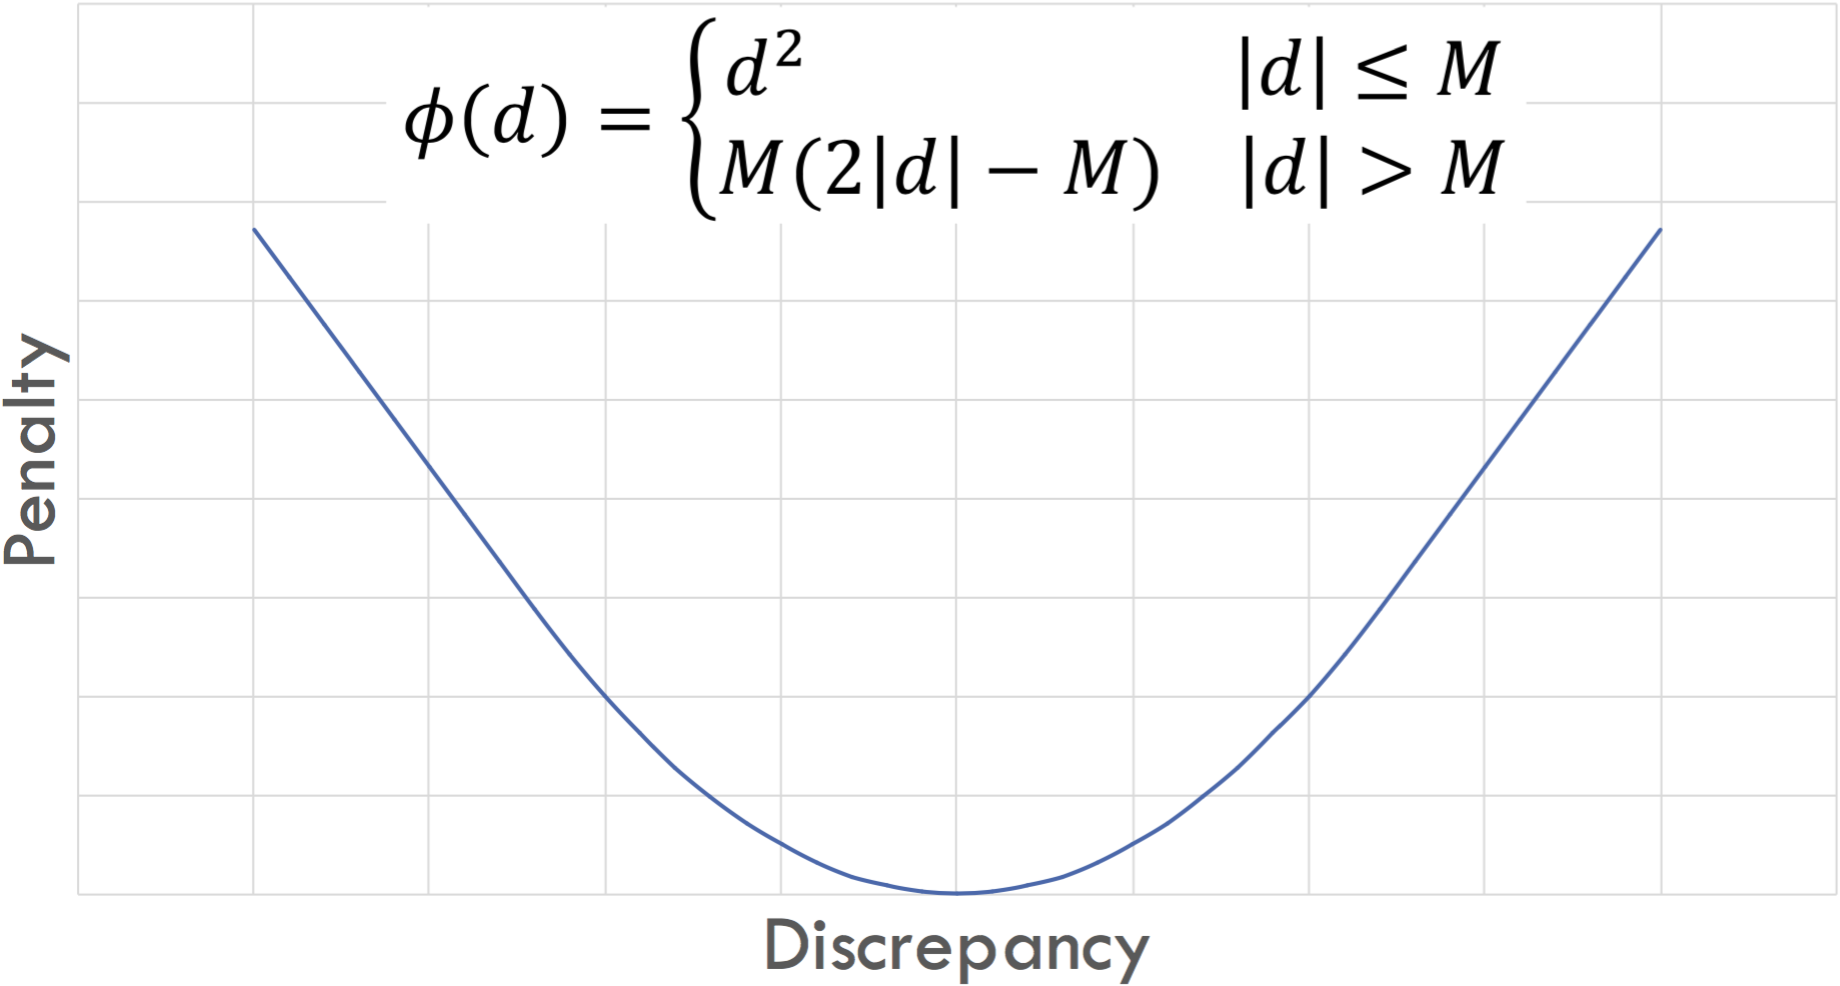
\includegraphics[scale=0.32]{pics/pen3.png}
\end{frame}

% \mynew
% \end{frame}





\section{References}
\begin{frame}
  \frametitle{References}
\tiny

%\input cwebmac
% This file is part of the Stanford GraphBase (c) Stanford University 1993
% This material goes at the beginning of all Stanford GraphBase CWEB files

\def\topofcontents{
  \leftline{\sc\today\ at \hours}\bigskip\bigskip
  \centerline{\titlefont\title}}

\font\ninett=cmtt9
\def\botofcontents{\vskip 0pt plus 1filll
    \ninerm\baselineskip10pt
    \noindent\copyright\ 1993 Stanford University
    \bigskip\noindent
    This file may be freely copied and distributed, provided that
    no changes whatsoever are made. All users are asked to help keep
    the Stanford GraphBase files consistent and ``uncorrupted,''
    identical everywhere in the world. Changes are permissible only
    if the modified file is given a new name, different from the names of
    existing files in the Stanford GraphBase, and only if the modified file is
    clearly identified as not being part of that GraphBase.
    (The {\ninett CWEB} system has a ``change file'' facility by
    which users can easily make minor alterations without modifying
    the master source files in any way. Everybody is supposed to use
    change files instead of changing the files.)
    The author has tried his best to produce correct and useful programs,
    in order to help promote computer science research,
    but no warranty of any kind should be assumed.
    \smallskip\noindent
    Preliminary work on the Stanford GraphBase project
    was supported in part by National Science
    Foundation grant CCR-86-10181.}

\def\prerequisite#1{\def\startsection{\noindent
    Important: Before reading {\sc\title},
    please read or at least skim the program for {\sc#1}.\bigskip
    \let\startsection=\stsec\stsec}}
\def\prerequisites#1#2{\def\startsection{\noindent
    Important: Before reading {\sc\title}, please read
    or at least skim the programs for {\sc#1} and {\sc#2}.\bigskip
    \let\startsection=\stsec\stsec}}



\def\title{GB\_\,BASIC}

\prerequisite{GB\_\,GRAPH}

\N{1}{1}Introduction. This GraphBase module contains six subroutines that
generate
standard graphs of various types, together with six routines that combine or
transform existing graphs.

Simple examples of the use of these routines can be found in the
demonstration programs {\sc QUEEN} and {\sc QUEEN\_WRAP}.

\Y\B\4\X1:\.{gb\_basic.h }\X${}\E{}$\6
\&{extern} \&{Graph} ${}{*}\\{board}(\,){}$;\C{ moves on generalized
chessboards }\6
\&{extern} \&{Graph} ${}{*}\\{simplex}(\,){}$;\C{ generalized triangular
configurations }\6
\&{extern} \&{Graph} ${}{*}\\{subsets}(\,){}$;\C{ patterns of subset
intersection }\6
\&{extern} \&{Graph} ${}{*}\\{perms}(\,){}$;\C{ permutations of a multiset }\6
\&{extern} \&{Graph} ${}{*}\\{parts}(\,){}$;\C{ partitions of an integer }\6
\&{extern} \&{Graph} ${}{*}\\{binary}(\,){}$;\C{ binary trees }\7
\&{extern} \&{Graph} ${}{*}\\{complement}(\,){}$;\C{ the complement of a graph
}\6
\&{extern} \&{Graph} ${}{*}\\{gunion}(\,){}$;\C{ the union of two graphs }\6
\&{extern} \&{Graph} ${}{*}\\{intersection}(\,){}$;\C{ the intersection of two
graphs }\6
\&{extern} \&{Graph} ${}{*}\\{lines}(\,){}$;\C{ the line graph of a graph }\6
\&{extern} \&{Graph} ${}{*}\\{product}(\,){}$;\C{ the product of two graphs }\6
\&{extern} \&{Graph} ${}{*}\\{induced}(\,){}$;\C{ a graph induced from another
}\par
\As7, 36, 41, 54, 63, 94, 100, 102\ETs104.\fi

\M{2}The \CEE/ file \.{gb\_basic.c} has the following overall shape:

\Y\B\8\#\&{include} \.{"gb\_graph.h"}\C{ we use the {\sc GB\_\,GRAPH} data
structures }\6
\ATH\7
\X3:Private variables\X\6
\X8:Basic subroutines\X\6
\X101:Applications of basic subroutines\X\par
\fi

\M{3}Several of the programs below allocate arrays that will be freed again
before the routine is finished.

\Y\B\4\X3:Private variables\X${}\E{}$\6
\&{static} \&{Area} \\{working\_storage};\par
\As5, 10\ETs51.
\U2.\fi

\M{4}If a graph-generating subroutine encounters a problem, it returns \PB{$%
\NULL$}
(that is, \.{NULL}), after putting a code number into the external variable
\PB{\\{panic\_code}}. This code number identifies the type of failure.
Otherwise the routine returns a pointer to the newly created graph, which
will be represented with the data structures explained in {\sc GB\_\,GRAPH}.
(The external variable \PB{\\{panic\_code}} is itself defined in {\sc GB\_%
\,GRAPH}.)

\Y\B\4\D$\\{panic}(\|c)$ \6
${}\{{}$\5
\1${}\\{panic\_code}\K\|c;{}$\6
\\{gb\_free}(\\{working\_storage});\6
${}\\{gb\_trouble\_code}\K\T{0};{}$\6
\&{return} ${}\NULL;{}$\6
\4${}\}{}$\2\par
\fi

\M{5}The names of vertices are sometimes formed from the names of other
vertices, or from potentially long sequences of numbers. We assemble
them in the \PB{\\{buffer}} array, which is sufficiently long that the
vast majority of applications will be unconstrained by size limitations.
The programs assume that \PB{\.{BUF\_SIZE}} is rather large, but in cases of
doubt they ensure that \PB{\.{BUF\_SIZE}} will never be exceeded.

\Y\B\4\D$\.{BUF\_SIZE}$ \5
\T{4096}\par
\Y\B\4\X3:Private variables\X${}\mathrel+\E{}$\6
\&{static} \&{char} \\{buffer}[\.{BUF\_SIZE}];\par
\fi

\N{1}{6}Grids and game boards. The subroutine call
\PB{$\\{board}(\\{n1},\\{n2},\\{n3},\\{n4},\\{piece},\\{wrap},\\{directed})$}
constructs a graph based on the moves of generalized chesspieces on a
generalized rectangular board. Each vertex of the graph corresponds to a
position on the board. Each arc of the graph corresponds to a move from
one position to another.

The first parameters, \PB{\\{n1}} through \PB{\\{n4}}, specify the size of the
board.
If, for example, a two-dimensional board with $n_1$ rows and $n_2$ columns
is desired, you set $\PB{\\{n1}}=n_1$, $\PB{\\{n2}}=n_2$, and $\PB{\\{n3}}=0$;
the resulting
graph will have $n_1n_2$ vertices. If you want a three-dimensional
board with $n_3$ layers, set $\PB{\\{n3}}=n_3$ and $n_4=0$. If you want
a 4-{\mc D} board, put the number of 4th coordinates in~\PB{\\{n4}}.
If you want a $d$-dimensional board with $2^d$ positions, set \PB{$\\{n1}\K%
\T{2}$}
and \PB{$\\{n2}\K{-}\|d$}.

In general, the \PB{\\{board}} subroutine determines the dimensions by scanning
the
sequence \PB{$(\\{n1},\\{n2},\\{n3},\\{n4},\T{0})$ $\K%
\hbox{$(n_1,n_2,n_3,n_4,0)$}$} from left to right
until coming to the first nonpositive parameter $n_{k+1}$. If $k=0$
(i.e., if \PB{$\\{n1}\Z\T{0}$}), the default size $8\times8$ will be used; this
is
an ordinary chessboard with 8~rows and 8~columns. Otherwise if $n_{k+1}=0$,
the board will have $k$~dimensions $n_1$, \dots,~$n_k$. Otherwise
we must have $n_{k+1}<0$; in this case, the board will have $d=\vert n_{k+1}
\vert$ dimensions, chosen as the first $d$ elements of the infinite
periodic sequence $(n_1,\ldots,n_k,n_1,\ldots,n_k,n_1,\ldots\,)$.
For example, the specification \PB{$(\\{n1},\\{n2},\\{n3},\\{n4})\K(\T{2},%
\T{3},\T{5},{-}\T{7})$} is about as
tricky as you can get. It produces a seven-dimensional board with
dimensions $(n_1,\ldots,n_7)=(2,3,5,2,3,5,2)$, hence a graph with
$2\cdot3\cdot5\cdot2\cdot3\cdot5\cdot2=1800$ vertices.

The \PB{\\{piece}} parameter specifies the legal moves of a generalized
chesspiece.
If \PB{$\\{piece}>\T{0}$}, a move from position~\PB{\|u} to position~\PB{\|v}
is considered legal
if and only if the Euclidean distance between points \PB{\|u} and~\PB{\|v} is
equal to $\sqrt{\vphantom1\smash{\PB{\\{piece}}}}$.
For example, if \PB{$\\{piece}\K\T{1}$} and if we have a
two-dimensional board, the legal moves from $(x,y)$ are to $(x,y\pm1)$ and
$(x\pm1,y)$; these are the moves of a so-called wazir, the only moves that
a king and a rook can both make. If \PB{$\\{piece}\K\T{2}$}, the legal moves
from $(x,y)$
are to $(x\pm1,y\pm1)$; these are the four moves that a king and a bishop
can both make. (A piece that can make only these moves was called a ``fers''
in ancient Muslim chess.) If \PB{$\\{piece}\K\T{5}$}, the legal moves are those
of a
knight, from $(x,y)$ to $(x\pm1,y\pm2)$ or to $(x\pm2,y\pm1)$. If \PB{$%
\\{piece}\K\T{3}$},
there are no legal moves on a two-dimensional board; but moves from
$(x,y,z)$ to $(x\pm1,y\pm1,z\pm1)$ would be legal in three dimensions.
If \PB{$\\{piece}\K\T{0}$}, it is changed to the default value \PB{$\\{piece}\K%
\T{1}$}.

If the value of \PB{\\{piece}} is negative, arbitrary multiples of the basic
moves
for $\vert\PB{\\{piece}}\vert$ are permitted. For example, \PB{$\\{piece}\K{-}%
\T{1}$} defines the
moves of a rook, from $(x,y)$ to $(x\pm a,y)$ or to $(x,y\pm a)$ for all
$a>0$; \PB{$\\{piece}\K{-}\T{2}$} defines the moves of a bishop, from $(x,y)$
to
$(x\pm a,y\pm a)$. The literature of ``fairy chess'' assigns standard names
to the following \PB{\\{piece}} values: $\rm wazir=1$, $\rm fers=2$, $\rm
dabbaba=4$,
$\rm knight=5$, $\rm alfil=8$, $\rm camel=10$, $\rm zebra=13$, $\rm giraffe
=17$, $\rm fiveleaper=25$, $\hbox{root-50-leaper}=50$, etc.; $\rm rook=-1$,
$\rm bishop=-2$, $\rm unicorn=-3$, $\rm dabbabarider=-4$, $\rm nightrider=-5$,
$\rm alfilrider=-8$, $\rm camelrider=-10$, etc.

To generate a board with the moves of a king, you can use the \PB{\\{gunion}}
subroutine below to take the union of boards with \PB{$\\{piece}\K\T{1}$} and
\PB{$\\{piece}\K\T{2}$}. Similarly, you can get queen moves by taking the union
of
boards with \PB{$\\{piece}\K{-}\T{1}$} and \PB{$\\{piece}\K{-}\T{2}$}.

If \PB{$\\{piece}>\T{0}$}, all arcs of the graph will have length~1. If \PB{$%
\\{piece}<\T{0}$}, the
length of each arc will be the number of multiples of a basic move that
produced the arc.

\fi

\M{7}If the \PB{\\{wrap}} parameter is nonzero, it specifies a subset of
coordinates
in which values are computed modulo the corresponding size.
For example, the coordinates $(x,y)$ for vertices on a two-dimensional
board are restricted to the range $0\le x<n_1$, $0\le y<n_2$; therefore
when \PB{$\\{wrap}\K\T{0}$}, a move from $(x,y)$ to $(x+\delta_1,y+\delta_2)$
is
legal only if $0\le x+\delta_1<n_1$ and $0\le y+\delta_2<n_2$.
But when \PB{$\\{wrap}\K\T{1}$}, the $x$~coordinates are allowed to ``wrap
around'';
the move would then be made to $((x+\delta_1)\bmod n_1,y+\delta_2)$,
provided that $0\le y+\delta_2<n_2$. Setting \PB{$\\{wrap}\K\T{1}$} effectively
makes the board into a cylinder instead of a rectangle. Similarly, the
$y$~coordinates are allowed to wrap around when \PB{$\\{wrap}\K\T{2}$}. Both
$x$ and
$y$ coordinates are treated modulo their corresponding sizes when
\PB{$\\{wrap}\K\T{3}$}; the board is then effectively a torus.  In general,
coordinates $k_1$, $k_2$, \dots~ will wrap around when
$\PB{\\{wrap}}=2^{k_1-1}+2^{k_2-1}+\cdots\,$. Setting \PB{$\\{wrap}\K{-}\T{1}$}
causes all
coordinates to be computed modulo their size.

The graph constructed by \PB{\\{board}} will be undirected unless \PB{$%
\\{directed}\I\T{0}$}.
Directed \PB{\\{board}} graphs will be acyclic when \PB{$\\{wrap}\K\T{0}$}, but
they may
have cycles when \PB{$\\{wrap}\I\T{0}$}. Precise rules defining the directed
arcs
are given below.

Several important special cases are worth noting. To get the complete graph
on \PB{\|n} vertices, you can say \PB{$\\{board}(\|n,\T{0},\T{0},\T{0},{-}%
\T{1},\T{0},\T{0})$}. To get the
transitive tournament on \PB{\|n} vertices, i.e., the directed graph
with arcs from \PB{\|u} to \PB{\|v} when \PB{$\|u<\|v$}, you can say \PB{$%
\\{board}(\|n,\T{0},\T{0},\T{0},{-}\T{1},\T{0},\T{1})$}.
To get the empty graph on \PB{\|n} vertices, you can say \PB{$\\{board}(\|n,%
\T{0},\T{0},\T{0},\T{2},\T{0},\T{0})$}.
To get a circuit (undirected) or a cycle (directed) of length~\PB{\|n},
you can say \PB{$\\{board}(\|n,\T{0},\T{0},\T{0},\T{1},\T{1},\T{0})$} and \PB{$%
\\{board}(\|n,\T{0},\T{0},\T{0},\T{1},\T{1},\T{1})$},
respectively.

\Y\B\4\X1:\.{gb\_basic.h }\X${}\mathrel+\E{}$\6
\8\#\&{define} \\{complete}(\|n) \5${}\\{board}((\&{long})(\|n),\39\T{0\$L},\39%
\T{0\$L},\39\T{0\$L},\39{-}\T{1\$L},\39\T{0\$L},\39\T{0\$L}){}$\6
\8\#\&{define} \\{transitive}(\|n) \5${}\\{board}((\&{long})(\|n),\39\T{0\$L},%
\39\T{0\$L},\39\T{0\$L},\39{-}\T{1\$L},\39\T{0\$L},\39\T{1\$L}){}$\6
\8\#\&{define} \\{empty}(\|n) \5${}\\{board}((\&{long})(\|n),\39\T{0\$L},\39%
\T{0\$L},\39\T{0\$L},\39\T{2\$L},\39\T{0\$L},\39\T{0\$L}){}$\6
\8\#\&{define} \\{circuit}(\|n) \5${}\\{board}((\&{long})(\|n),\39\T{0\$L},\39%
\T{0\$L},\39\T{0\$L},\39\T{1\$L},\39\T{1\$L},\39\T{0\$L}){}$\6
\8\#\&{define} \\{cycle}(\|n) \5${}\\{board}((\&{long})(\|n),\39\T{0\$L},\39%
\T{0\$L},\39\T{0\$L},\39\T{1\$L},\39\T{1\$L},\39\T{1\$L}){}$\par
\fi

\M{8}\B\X8:Basic subroutines\X${}\E{}$\6
\&{Graph} ${}{*}\\{board}(\\{n1},\39\\{n2},\39\\{n3},\39\\{n4},\39\\{piece},\39%
\\{wrap},\39\\{directed}){}$\1\1\6
\&{long} \\{n1}${},{}$ \\{n2}${},{}$ \\{n3}${},{}$ \\{n4};\C{ size of board
desired }\6
\&{long} \\{piece};\C{ type of moves desired }\6
\&{long} \\{wrap};\C{ mask for coordinate positions that wrap around }\6
\&{long} \\{directed};\C{ should the graph be directed? }\2\2\6
${}\{{}$\5
\1\X9:Vanilla local variables\X\5
\hbox{}\6{}\&{long} \|n;\C{ total number of vertices }\6
\&{long} \|p;\C{ $\vert\PB{\\{piece}}\vert$ }\6
\&{long} \|l;\C{ length of current arc }\7
\X11:Normalize the board-size parameters\X;\6
\X13:Set up a graph with \PB{\|n} vertices\X;\6
\X15:Insert arcs or edges for all legal moves\X;\6
\&{if} (\\{gb\_trouble\_code})\5
${}\{{}$\1\6
\\{gb\_recycle}(\\{new\_graph});\6
\\{panic}(\\{alloc\_fault});\C{ alas, we ran out of memory somewhere back there
}\6
\4${}\}{}$\2\6
\&{return} \\{new\_graph};\6
\4${}\}{}$\2\par
\As26, 37, 43, 55, 64, 74, 78, 81, 87, 95\ETs105.
\U2.\fi

\M{9}Most of the subroutines in {\sc GB\_\,BASIC} use the following local
variables.

\Y\B\4\X9:Vanilla local variables\X${}\E{}$\6
\&{Graph} ${}{*}\\{new\_graph}{}$;\C{ the graph being constructed }\6
\&{register} \&{long} \|i${},{}$ \|j${},{}$ \|k;\C{ all-purpose indices }\6
\&{register} \&{long} \|d;\C{ the number of dimensions }\6
\&{register} \&{Vertex} ${}{*}\|v{}$;\C{ the current vertex of interest }\6
\&{register} \&{long} \|s;\C{ accumulator }\par
\Us8, 26, 37, 43, 55, 64, 74, 78, 81, 87, 95\ETs105.\fi

\M{10}Several arrays will facilitate the calculations that \PB{\\{board}} needs
to make.
The number of distinct values in coordinate position~$k$ will be \PB{\\{nn}[%
\|k]};
this coordinate position will wrap around if and only if \PB{$\\{wr}[\|k]\I%
\T{0}$}.
The current moves under consideration will be from $(x_1,\ldots,x_d)$
to $(x_1+\delta_1,\ldots, x_d+\delta_d)$, where $\delta_k$ is stored
in \PB{\\{del}[\|k]}. An auxiliary array \PB{\\{sig}} holds the sums
$\sigma_k=\delta_1^2+\cdots+\delta_{k-1}^2$.  Additional arrays \PB{\\{xx}}
and \PB{\\{yy}} hold coordinates of vertices before and after a move is made.

Some of these arrays are also used for other purposes by other programs
besides \PB{\\{board}}; we will meet those programs later.

We limit the number of dimensions to 91 or less. This is hardly a limitation,
since the number of vertices would be astronomical even if the dimensionality
were only half this big. But some of our later programs will be able
to make good use of 40 or 50 dimensions and perhaps more; the number 91
is an upper limit imposed by the number of standard printable characters
(see the convention for vertex names in the \PB{\\{perms}} routine).

\Y\B\4\D$\.{MAX\_D}$ \5
\T{91}\par
\Y\B\4\X3:Private variables\X${}\mathrel+\E{}$\6
\&{static} \&{long} ${}\\{nn}[\.{MAX\_D}+\T{1}]{}$;\C{ component sizes }\6
\&{static} \&{long} ${}\\{wr}[\.{MAX\_D}+\T{1}]{}$;\C{ does this component wrap
around? }\6
\&{static} \&{long} ${}\\{del}[\.{MAX\_D}+\T{1}]{}$;\C{ displacements for the
current move }\6
\&{static} \&{long} ${}\\{sig}[\.{MAX\_D}+\T{2}]{}$;\C{ partial sums of squares
of displacements }\6
\&{static} \&{long} ${}\\{xx}[\.{MAX\_D}+\T{1}],{}$ ${}\\{yy}[\.{MAX\_D}+%
\T{1}]{}$;\C{ coordinate values }\par
\fi

\M{11}\B\X11:Normalize the board-size parameters\X${}\E{}$\6
\&{if} ${}(\\{piece}\E\T{0}){}$\1\5
${}\\{piece}\K\T{1};{}$\2\6
\&{if} ${}(\\{n1}\Z\T{0}){}$\5
${}\{{}$\5
\1${}\\{n1}\K\\{n2}\K\T{8}{}$;\5
${}\\{n3}\K\T{0}{}$;\5
${}\}{}$\2\6
${}\\{nn}[\T{1}]\K\\{n1};{}$\6
\&{if} ${}(\\{n2}\Z\T{0}){}$\5
${}\{{}$\5
\1${}\|k\K\T{2}{}$;\5
${}\|d\K{-}\\{n2}{}$;\5
${}\\{n3}\K\\{n4}\K\T{0}{}$;\5
${}\}{}$\2\6
\&{else}\5
${}\{{}$\1\6
${}\\{nn}[\T{2}]\K\\{n2};{}$\6
\&{if} ${}(\\{n3}\Z\T{0}){}$\5
${}\{{}$\5
\1${}\|k\K\T{3}{}$;\5
${}\|d\K{-}\\{n3}{}$;\5
${}\\{n4}\K\T{0}{}$;\5
${}\}{}$\2\6
\&{else}\5
${}\{{}$\1\6
${}\\{nn}[\T{3}]\K\\{n3};{}$\6
\&{if} ${}(\\{n4}\Z\T{0}){}$\5
${}\{{}$\5
\1${}\|k\K\T{4}{}$;\5
${}\|d\K{-}\\{n4}{}$;\5
${}\}{}$\2\6
\&{else}\5
${}\{{}$\5
\1${}\\{nn}[\T{4}]\K\\{n4}{}$;\5
${}\|d\K\T{4}{}$;\5
\&{goto} \\{done};\5
${}\}{}$\2\6
\4${}\}{}$\2\6
\4${}\}{}$\2\6
\&{if} ${}(\|d\E\T{0}){}$\5
${}\{{}$\5
\1${}\|d\K\|k-\T{1}{}$;\5
\&{goto} \\{done};\5
${}\}{}$\2\6
\X12:Compute component sizes periodically for \PB{\|d} dimensions\X;\6
\\{done}:\C{ now \PB{\\{nn}[\T{1}]} through \PB{\\{nn}[\|d]} are set up }\par
\U8.\fi

\M{12}At this point, \PB{\\{nn}[\T{1}]} through \PB{$\\{nn}[\|k-\T{1}]$} are
the component sizes
that should be replicated periodically. In unusual cases, the number
of dimensions might not be as large as the number of specifications.

\Y\B\4\X12:Compute component sizes periodically for \PB{\|d} dimensions\X${}%
\E{}$\6
\&{if} ${}(\|d>\.{MAX\_D}){}$\1\5
\\{panic}(\\{bad\_specs});\C{ too many dimensions }\2\6
\&{for} ${}(\|j\K\T{1};{}$ ${}\|k\Z\|d;{}$ ${}\|j\PP,\39\|k\PP){}$\1\5
${}\\{nn}[\|k]\K\\{nn}[\|j]{}$;\2\par
\Us11\ET27.\fi

\M{13}We want to make the subroutine idiot-proof, so we use floating-point
arithmetic to make sure that boards with more than a billion cells have
not been specified.

\Y\B\4\D$\.{MAX\_NNN}$ \5
\T{1000000000.0}\par
\Y\B\4\X13:Set up a graph with \PB{\|n} vertices\X${}\E{}$\6
${}\{{}$\5
\1\&{float} \\{nnn};\C{ approximate size }\7
\&{for} ${}(\|n\K\T{1},\39\\{nnn}\K\T{1.0},\39\|j\K\T{1};{}$ ${}\|j\Z\|d;{}$
${}\|j\PP){}$\5
${}\{{}$\1\6
${}\\{nnn}\MRL{*{\K}}{}$(\&{float}) \\{nn}[\|j];\6
\&{if} ${}(\\{nnn}>\.{MAX\_NNN}){}$\1\5
\\{panic}(\\{very\_bad\_specs});\C{ way too big }\2\6
${}\|n\MRL{*{\K}}\\{nn}[\|j]{}$;\C{ this multiplication cannot cause integer
overflow }\6
\4${}\}{}$\2\6
${}\\{new\_graph}\K\\{gb\_new\_graph}(\|n);{}$\6
\&{if} ${}(\\{new\_graph}\E\NULL){}$\1\5
\\{panic}(\\{no\_room});\C{ out of memory before we're even started }\2\6
${}\\{sprintf}(\\{new\_graph}\MG\\{id},\39\.{"board(\%ld,\%ld,\%ld,\%}\)\.{ld,%
\%ld,\%ld,\%d)"},\39\\{n1},\39\\{n2},\39\\{n3},\39\\{n4},\39\\{piece},\39%
\\{wrap},\39\\{directed}\?\T{1}:\T{0});{}$\6
${}\\{strcpy}(\\{new\_graph}\MG\\{util\_types},\39\.{"ZZZIIIZZZZZZZZ"});{}$\6
\X14:Give names to the vertices\X;\6
\4${}\}{}$\2\par
\U8.\fi

\M{14}The symbolic name of a board position like $(3,1)$ will be the string
`\.{3.1}'. The first three coordinates are also stored as integers, in
utility fields \PB{$\|x.\|I$}, \PB{$\|y.\|I$}, and \PB{$\|z.\|I$}, because
immediate access to
those values will be helpful in certain applications. (The coordinates can,
of course, always be recovered in a slower fashion from the vertex name,
via \PB{\\{sscanf}}.)

The process of assigning coordinate values and names is equivalent to
adding unity in a mixed-radix number system. Vertex $(x_1,\ldots,x_d)$
will be in position $x_1n_2\ldots n_d+\cdots+x_{d-1}n_d+x_d$ relative
to the first vertex of the new graph; therefore it is also possible to
deduce the coordinates of a vertex from its address.

\Y\B\4\X14:Give names to the vertices\X${}\E{}$\6
${}\{{}$\5
\1\&{register} \&{char} ${}{*}\|q{}$;\C{ string pointer }\7
${}\\{nn}[\T{0}]\K\\{xx}[\T{0}]\K\\{xx}[\T{1}]\K\\{xx}[\T{2}]\K\\{xx}[\T{3}]\K%
\T{0};{}$\6
\&{for} ${}(\|k\K\T{4};{}$ ${}\|k\Z\|d;{}$ ${}\|k\PP){}$\1\5
${}\\{xx}[\|k]\K\T{0};{}$\2\6
\&{for} ${}(\|v\K\\{new\_graph}\MG\\{vertices};{}$  ; ${}\|v\PP){}$\5
${}\{{}$\1\6
${}\|q\K\\{buffer};{}$\6
\&{for} ${}(\|k\K\T{1};{}$ ${}\|k\Z\|d;{}$ ${}\|k\PP){}$\5
${}\{{}$\1\6
${}\\{sprintf}(\|q,\39\.{".\%ld"},\39\\{xx}[\|k]);{}$\6
\&{while} ${}({*}\|q){}$\1\5
${}\|q\PP;{}$\2\6
\4${}\}{}$\2\6
${}\|v\MG\\{name}\K\\{gb\_save\_string}({\AND}\\{buffer}[\T{1}]){}$;\C{ omit %
\PB{\\{buffer}[\T{0}]}, which is \PB{\.{'.'}} }\6
${}\|v\MG\|x.\|I\K\\{xx}[\T{1}]{}$;\5
${}\|v\MG\|y.\|I\K\\{xx}[\T{2}]{}$;\5
${}\|v\MG\|z.\|I\K\\{xx}[\T{3}];{}$\6
\&{for} ${}(\|k\K\|d;{}$ ${}\\{xx}[\|k]+\T{1}\E\\{nn}[\|k];{}$ ${}\|k\MM){}$\1\5
${}\\{xx}[\|k]\K\T{0};{}$\2\6
\&{if} ${}(\|k\E\T{0}){}$\1\5
\&{break};\C{ a ``carry'' has occurred all the way to the left }\2\6
${}\\{xx}[\|k]\PP{}$;\C{ increase coordinate \PB{\|k} }\6
\4${}\}{}$\2\6
\4${}\}{}$\2\par
\U13.\fi

\M{15}Now we come to a slightly tricky part of the routine: the move generator.
Let $p=\vert\PB{\\{piece}}\vert$. The outer loop of this procedure runs through
all
solutions of the equation $\delta_1^2+\cdots+\delta_d^2=p$, where the
$\delta$'s are nonnegative integers. Within that loop, we attach signs
to the $\delta$'s, but we always leave $\delta_k$ positive if $\delta_1=
\cdots=\delta_{k-1}=0$. For every such vector~$\delta$, we generate moves
from \PB{\|v} to $v+\delta$ for every vertex \PB{\|v}. When \PB{$\\{directed}\K%
\T{0}$},
we use \PB{\\{gb\_new\_edge}} instead of \PB{\\{gb\_new\_arc}}, so that the
reverse arc
from $v+\delta$ to~\PB{\|v} is also generated.

\Y\B\4\X15:Insert arcs or edges for all legal moves\X${}\E{}$\6
\X16:Initialize the \PB{\\{wr}}, \PB{\\{sig}}, and \PB{\\{del}} tables\X;\6
${}\|p\K\\{piece};{}$\6
\&{if} ${}(\|p<\T{0}){}$\1\5
${}\|p\K{-}\|p;{}$\2\6
\&{while} (\T{1})\5
${}\{{}$\1\6
\X17:Advance to the next nonnegative \PB{\\{del}} vector, or \PB{\&{break}} if
done\X;\6
\&{while} (\T{1})\5
${}\{{}$\1\6
\X19:Generate moves for the current \PB{\\{del}} vector\X;\6
\X18:Advance to the next signed \PB{\\{del}} vector, or restore \PB{\\{del}} to
nonnegative values and \PB{\&{break}}\X;\6
\4${}\}{}$\2\6
\4${}\}{}$\2\par
\U8.\fi

\M{16}The \CEE/ language does not define \PB{$\GG$} unambiguously. If \PB{\|w}
is negative,
the assignment `\PB{$\|w\MRL{{\GG}{\K}}\T{1}$}' here should keep \PB{\|w}
negative.
(However, this technicality doesn't matter except in highly unusual cases
when there are more than 32 dimensions.)

\Y\B\4\X16:Initialize the \PB{\\{wr}}, \PB{\\{sig}}, and \PB{\\{del}} tables%
\X${}\E{}$\6
${}\{{}$\5
\1\&{register} \&{long} \|w${}\K\\{wrap};{}$\7
\&{for} ${}(\|k\K\T{1};{}$ ${}\|k\Z\|d;{}$ ${}\|k\PP,\39\|w\MRL{{\GG}{\K}}%
\T{1}){}$\5
${}\{{}$\1\6
${}\\{wr}[\|k]\K\|w\AND\T{1};{}$\6
${}\\{del}[\|k]\K\\{sig}[\|k]\K\T{0};{}$\6
\4${}\}{}$\2\6
${}\\{sig}[\T{0}]\K\\{del}[\T{0}]\K\\{sig}[\|d+\T{1}]\K\T{0};{}$\6
\4${}\}{}$\2\par
\U15.\fi

\M{17}The \PB{\\{sig}} array makes it easy to backtrack through all partitions
of \PB{\|p} into an ordered sum of squares.

\Y\B\4\X17:Advance to the next nonnegative \PB{\\{del}} vector, or \PB{%
\&{break}} if done\X${}\E{}$\6
\&{for} ${}(\|k\K\|d;{}$ ${}\\{sig}[\|k]+(\\{del}[\|k]+\T{1})*(\\{del}[\|k]+%
\T{1})>\|p;{}$ ${}\|k\MM){}$\1\5
${}\\{del}[\|k]\K\T{0};{}$\2\6
\&{if} ${}(\|k\E\T{0}){}$\1\5
\&{break};\2\6
${}\\{del}[\|k]\PP;{}$\6
${}\\{sig}[\|k+\T{1}]\K\\{sig}[\|k]+\\{del}[\|k]*\\{del}[\|k];{}$\6
\&{for} ${}(\|k\PP;{}$ ${}\|k\Z\|d;{}$ ${}\|k\PP){}$\1\5
${}\\{sig}[\|k+\T{1}]\K\\{sig}[\|k];{}$\2\6
\&{if} ${}(\\{sig}[\|d+\T{1}]<\|p){}$\1\5
\&{continue};\2\par
\U15.\fi

\M{18}\B\X18:Advance to the next signed \PB{\\{del}} vector, or restore \PB{%
\\{del}} to nonnegative values and \PB{\&{break}}\X${}\E{}$\6
\&{for} ${}(\|k\K\|d;{}$ ${}\\{del}[\|k]\Z\T{0};{}$ ${}\|k\MM){}$\1\5
${}\\{del}[\|k]\K{-}\\{del}[\|k];{}$\2\6
\&{if} ${}(\\{sig}[\|k]\E\T{0}){}$\1\5
\&{break};\C{ all but \PB{\\{del}[\|k]} were negative or zero }\2\6
${}\\{del}[\|k]\K{-}\\{del}[\|k]{}$;\C{ some entry preceding \PB{\\{del}[\|k]}
is positive }\par
\U15.\fi

\M{19}We use the mixed-radix addition technique again when generating moves.

\Y\B\4\X19:Generate moves for the current \PB{\\{del}} vector\X${}\E{}$\6
\&{for} ${}(\|k\K\T{1};{}$ ${}\|k\Z\|d;{}$ ${}\|k\PP){}$\1\5
${}\\{xx}[\|k]\K\T{0};{}$\2\6
\&{for} ${}(\|v\K\\{new\_graph}\MG\\{vertices};{}$  ; ${}\|v\PP){}$\5
${}\{{}$\1\6
\X20:Generate moves from \PB{\|v} corresponding to \PB{\\{del}}\X;\6
\&{for} ${}(\|k\K\|d;{}$ ${}\\{xx}[\|k]+\T{1}\E\\{nn}[\|k];{}$ ${}\|k\MM){}$\1\5
${}\\{xx}[\|k]\K\T{0};{}$\2\6
\&{if} ${}(\|k\E\T{0}){}$\1\5
\&{break};\C{ a ``carry'' has occurred all the way to the left }\2\6
${}\\{xx}[\|k]\PP{}$;\C{ increase coordinate \PB{\|k} }\6
\4${}\}{}$\2\par
\U15.\fi

\M{20}The legal moves when \PB{\\{piece}} is negative are derived as follows,
in
the presence of possible wraparound: Starting at $(x_1,\ldots,x_d)$, we
move to $(x_1+\delta_1,\ldots,x_d+\delta_d)$, $(x_1+2\delta_1,\ldots,
x_d+2\delta_d)$,~\dots, until either coming to a position with a nonwrapped
coordinate out of range or coming back to the original point.

A subtle technicality should be noted: When coordinates are wrapped and
\PB{$\\{piece}>\T{0}$}, self-loops are possible---for example, in \PB{$%
\\{board}(\T{1},\T{0},\T{0},\T{0},\T{1},\T{1},\T{1})$}.
But self-loops never arise when \PB{$\\{piece}<\T{0}$}.

\Y\B\4\X20:Generate moves from \PB{\|v} corresponding to \PB{\\{del}}\X${}\E{}$%
\6
\&{for} ${}(\|k\K\T{1};{}$ ${}\|k\Z\|d;{}$ ${}\|k\PP){}$\1\5
${}\\{yy}[\|k]\K\\{xx}[\|k]+\\{del}[\|k];{}$\2\6
\&{for} ${}(\|l\K\T{1};{}$  ; ${}\|l\PP){}$\5
${}\{{}$\1\6
\X22:Correct for wraparound, or \PB{\&{goto} \\{no\_more}} if off the board\X;\6
\&{if} ${}(\\{piece}<\T{0}){}$\1\5
\X21:Go to \PB{\\{no\_more}} if \PB{$\\{yy}\K\\{xx}$}\X;\2\6
\X23:Record a legal move from \PB{\\{xx}} to \PB{\\{yy}}\X;\6
\&{if} ${}(\\{piece}>\T{0}){}$\1\5
\&{goto} \\{no\_more};\2\6
\&{for} ${}(\|k\K\T{1};{}$ ${}\|k\Z\|d;{}$ ${}\|k\PP){}$\1\5
${}\\{yy}[\|k]\MRL{+{\K}}\\{del}[\|k];{}$\2\6
\4${}\}{}$\2\6
\4\\{no\_more}:\par
\U19.\fi

\M{21}\B\X21:Go to \PB{\\{no\_more}} if \PB{$\\{yy}\K\\{xx}$}\X${}\E{}$\6
${}\{{}$\1\6
\&{for} ${}(\|k\K\T{1};{}$ ${}\|k\Z\|d;{}$ ${}\|k\PP){}$\1\6
\&{if} ${}(\\{yy}[\|k]\I\\{xx}[\|k]){}$\1\5
\&{goto} \\{unequal};\2\2\6
\&{goto} \\{no\_more};\6
\4\\{unequal}:\5
;\6
\4${}\}{}$\2\par
\U20.\fi

\M{22}\B\X22:Correct for wraparound, or \PB{\&{goto} \\{no\_more}} if off the
board\X${}\E{}$\6
\&{for} ${}(\|k\K\T{1};{}$ ${}\|k\Z\|d;{}$ ${}\|k\PP){}$\5
${}\{{}$\1\6
\&{if} ${}(\\{yy}[\|k]<\T{0}){}$\5
${}\{{}$\1\6
\&{if} ${}(\R\\{wr}[\|k]){}$\1\5
\&{goto} \\{no\_more};\2\6
\&{do}\5
${}\\{yy}[\|k]\MRL{+{\K}}\\{nn}[\|k]{}$;\5
\5
\&{while} ${}(\\{yy}[\|k]<\T{0});{}$\6
\4${}\}{}$\5
\2\&{else} \&{if} ${}(\\{yy}[\|k]\G\\{nn}[\|k]){}$\5
${}\{{}$\1\6
\&{if} ${}(\R\\{wr}[\|k]){}$\1\5
\&{goto} \\{no\_more};\2\6
\&{do}\5
${}\\{yy}[\|k]\MRL{-{\K}}\\{nn}[\|k]{}$;\5
\5
\&{while} ${}(\\{yy}[\|k]\G\\{nn}[\|k]);{}$\6
\4${}\}{}$\2\6
\4${}\}{}$\2\par
\U20.\fi

\M{23}\B\X23:Record a legal move from \PB{\\{xx}} to \PB{\\{yy}}\X${}\E{}$\6
\&{for} ${}(\|k\K\T{2},\39\|j\K\\{yy}[\T{1}];{}$ ${}\|k\Z\|d;{}$ ${}\|k\PP){}$%
\1\5
${}\|j\K\\{nn}[\|k]*\|j+\\{yy}[\|k];{}$\2\6
\&{if} (\\{directed})\1\5
${}\\{gb\_new\_arc}(\|v,\39\\{new\_graph}\MG\\{vertices}+\|j,\39\|l);{}$\2\6
\&{else}\1\5
${}\\{gb\_new\_edge}(\|v,\39\\{new\_graph}\MG\\{vertices}+\|j,\39\|l){}$;\2\par
\U20.\fi

\N{1}{24}Generalized triangular boards. The subroutine call
\PB{$\\{simplex}(\|n,\\{n0},\\{n1},\\{n2},\\{n3},\\{n4},\\{directed})$} creates
a graph based on
generalized triangular or tetrahedral configurations. Such graphs are
similar in spirit to the game boards created by \PB{\\{board}}, but they
pertain to nonrectangular grids like those in Chinese checkers. As
with \PB{\\{board}} in the case \PB{$\\{piece}\K\T{1}$}, the vertices represent
board positions
and the arcs run from board positions to their nearest neighbors. Each arc has
length~1.{\tolerance=1000\par}

More formally, the vertices can be defined as sequences of nonnegative
integers $(x_0,x_1,\ldots,x_d)$ whose sum is~\PB{\|n}, where two sequences
are considered adjacent if and only if they differ by $\pm1$ in exactly
two components---equivalently, if the Euclidean distance between them
is~$\sqrt2$. When $d=2$, for example, the vertices can be visualized
as a triangular array
$$\vcenter{\halign{&\hbox to 2em{\hss$#$\hss}\cr
&&&(0,0,3)\cr
&&(0,1,2)&&(1,0,2)\cr
&(0,2,1)&&(1,1,1)&&(2,0,1)\cr
(0,3,0)&&(1,2,0)&&(2,1,0)&&(3,0,0)\cr}}$$
containing $(n+1)(n+2)/2$ elements, illustrated here when $n=3$; each vertex of
the array has up to 6 neighbors. When $d=3$ the vertices form a tetrahedral
array, a stack of triangular layers, and they can have as many as 12
neighbors. In general, a vertex in a $d$-simplicial array will have up to
$d(d+1)$ neighbors.

If the \PB{\\{directed}} parameter is nonzero, arcs run only from vertices to
neighbors that are lexicographically greater---for example, downward
or to the right in the triangular array shown. The directed graph is
therefore acyclic, and a vertex of a $d$-simplicial array has
out-degree at most $d(d+1)/2$.

\fi

\M{25}The first parameter, \PB{\|n}, specifies the sum of the coordinates
$(x_0,x_1,\ldots,x_d)$. The following parameters \PB{\\{n0}} through \PB{%
\\{n4}}
specify upper bounds on those coordinates, and they also specify the
dimensionality~\PB{\|d}.

If, for example, \PB{\\{n0}}, \PB{\\{n1}}, and \PB{\\{n2}} are positive while %
\PB{$\\{n3}\K\T{0}$}, the
value of~\PB{\|d} will be~2 and the coordinates will be constrained to
satisfy $0\le x_0\le\PB{\\{n0}}$, $0\le x_1\le\PB{\\{n1}}$, $0\le x_2\le\PB{%
\\{n2}}$. These
upper bounds essentially lop off the corners of the triangular array.
We obtain a hexagonal board with $6m$ boundary cells by asking for
\PB{$\\{simplex}(\T{3}\|m,\T{2}\|m,\T{2}\|m,\T{2}\|m,\T{0},\T{0},\T{0})$}. We
obtain the diamond-shaped board used
in the game of Hex [Martin Gardner, {\sl The Scientific American
Book of Mathematical Puzzles {\char`\&} Diversions\/} (Simon {\char`\&}
Schuster, 1959), Chapter~8] by calling \PB{$\\{simplex}(\T{20},\T{10},\T{20},%
\T{10},\T{0},\T{0},\T{0})$}.

In general, \PB{\\{simplex}} determines \PB{\|d} and upper bounds $(n_0,n_1,%
\ldots,n_d)$
in the following way: Let the first nonpositive entry of the sequence
\PB{$(\\{n0},\\{n1},\\{n2},\\{n3},\\{n4},\T{0})$}$%
\null=(n_0,n_1,n_2,n_3,n_4,0)$ be~$n_k$. If $k>0$
and $n_k=0$, the value of~$d$ will be $k-1$ and the coordinates will be
bounded by the given numbers $(n_0,\ldots,n_d)$. If $k>0$ and $n_k<0$,
the value of~$d$ will be $\vert n_k\vert$ and the coordinates will be
bounded by the first $d+1$ elements of the infinite periodic sequence
$(n_0,\ldots,n_{k-1},n_0,\ldots,n_{k-1},n_0,\ldots\,)$. If $k=0$ and
$n_0<0$, the value of~$d$ will be $\vert n_0\vert$ and the coordinates
will be unbounded; equivalently, we may set $n_0=\cdots=n_d=n$. In
this case the number of vertices will be $n+d\choose d$. Finally,
if $k=0$ and $n_0=0$, we have the default case of a triangular array
with $3n$ boundary cells, exactly as if $n_0=-2$.

For example, the specification \PB{$\\{n0}\K\T{3}$}, \PB{$\\{n1}\K{-}\T{5}$}
will produce all vertices
$(x_0,x_1,\ldots,x_5)$ such that $x_0+x_1+\cdots+x_5=n$ and $0\le x_j\le3$.
The specification \PB{$\\{n0}\K\T{1}$}, \PB{$\\{n1}\K{-}\|d$} will essentially
produce all $n$-element
subsets of the $(d+1)$-element set $\{0,1,\ldots,d\}$, because we can
regard an element~$k$ as being present in the set if $x_k=1$ and absent
if $x_k=0$. In that case two subsets are adjacent if and only if
they have exactly $n-1$ elements in common.

\fi

\M{26}\B\X8:Basic subroutines\X${}\mathrel+\E{}$\6
\&{Graph} ${}{*}\\{simplex}(\|n,\39\\{n0},\39\\{n1},\39\\{n2},\39\\{n3},\39%
\\{n4},\39\\{directed}){}$\1\1\6
\&{unsigned} \&{long} \|n;\C{ the constant sum of all coordinates }\6
\&{long} \\{n0}${},{}$ \\{n1}${},{}$ \\{n2}${},{}$ \\{n3}${},{}$ \\{n4};\C{
constraints on coordinates }\6
\&{long} \\{directed};\C{ should the graph be directed? }\2\2\6
${}\{{}$\5
\1\X9:Vanilla local variables\X\7
\X27:Normalize the simplex parameters\X;\6
\X28:Create a graph with one vertex for each point\X;\6
\X31:Name the points and create the arcs or edges\X;\6
\&{if} (\\{gb\_trouble\_code})\5
${}\{{}$\1\6
\\{gb\_recycle}(\\{new\_graph});\6
\\{panic}(\\{alloc\_fault});\C{ darn, we ran out of memory somewhere back there
}\6
\4${}\}{}$\2\6
\&{return} \\{new\_graph};\6
\4${}\}{}$\2\par
\fi

\M{27}\B\X27:Normalize the simplex parameters\X${}\E{}$\6
\&{if} ${}(\\{n0}\E\T{0}){}$\1\5
${}\\{n0}\K{-}\T{2};{}$\2\6
\&{if} ${}(\\{n0}<\T{0}){}$\5
${}\{{}$\5
\1${}\|k\K\T{2}{}$;\5
${}\\{nn}[\T{0}]\K\|n{}$;\5
${}\|d\K{-}\\{n0}{}$;\5
${}\\{n1}\K\\{n2}\K\\{n3}\K\\{n4}\K\T{0}{}$;\5
${}\}{}$\2\6
\&{else}\5
${}\{{}$\1\6
\&{if} ${}(\\{n0}>\|n){}$\1\5
${}\\{n0}\K\|n;{}$\2\6
${}\\{nn}[\T{0}]\K\\{n0};{}$\6
\&{if} ${}(\\{n1}\Z\T{0}){}$\5
${}\{{}$\5
\1${}\|k\K\T{2}{}$;\5
${}\|d\K{-}\\{n1}{}$;\5
${}\\{n2}\K\\{n3}\K\\{n4}\K\T{0}{}$;\5
${}\}{}$\2\6
\&{else}\5
${}\{{}$\1\6
\&{if} ${}(\\{n1}>\|n){}$\1\5
${}\\{n1}\K\|n;{}$\2\6
${}\\{nn}[\T{1}]\K\\{n1};{}$\6
\&{if} ${}(\\{n2}\Z\T{0}){}$\5
${}\{{}$\5
\1${}\|k\K\T{3}{}$;\5
${}\|d\K{-}\\{n2}{}$;\5
${}\\{n3}\K\\{n4}\K\T{0}{}$;\5
${}\}{}$\2\6
\&{else}\5
${}\{{}$\1\6
\&{if} ${}(\\{n2}>\|n){}$\1\5
${}\\{n2}\K\|n;{}$\2\6
${}\\{nn}[\T{2}]\K\\{n2};{}$\6
\&{if} ${}(\\{n3}\Z\T{0}){}$\5
${}\{{}$\5
\1${}\|k\K\T{4}{}$;\5
${}\|d\K{-}\\{n3}{}$;\5
${}\\{n4}\K\T{0}{}$;\5
${}\}{}$\2\6
\&{else}\5
${}\{{}$\1\6
\&{if} ${}(\\{n3}>\|n){}$\1\5
${}\\{n3}\K\|n;{}$\2\6
${}\\{nn}[\T{3}]\K\\{n3};{}$\6
\&{if} ${}(\\{n4}\Z\T{0}){}$\5
${}\{{}$\5
\1${}\|k\K\T{5}{}$;\5
${}\|d\K{-}\\{n4}{}$;\5
${}\}{}$\2\6
\&{else}\5
${}\{{}$\5
\1\&{if} ${}(\\{n4}>\|n){}$\1\5
${}\\{n4}\K\|n;{}$\2\6
${}\\{nn}[\T{4}]\K\\{n4}{}$;\5
${}\|d\K\T{4}{}$;\5
\&{goto} \\{done};\5
${}\}{}$\2\6
\4${}\}{}$\2\6
\4${}\}{}$\2\6
\4${}\}{}$\2\6
\4${}\}{}$\2\6
\&{if} ${}(\|d\E\T{0}){}$\5
${}\{{}$\5
\1${}\|d\K\|k-\T{2}{}$;\5
\&{goto} \\{done};\5
${}\}{}$\2\6
${}\\{nn}[\|k-\T{1}]\K\\{nn}[\T{0}];{}$\6
\X12:Compute component sizes periodically for \PB{\|d} dimensions\X;\6
\\{done}:\C{ now \PB{\\{nn}[\T{0}]} through \PB{\\{nn}[\|d]} are set up }\par
\Us26, 37\ETs44.\fi

\M{28}\B\X28:Create a graph with one vertex for each point\X${}\E{}$\6
\X29:Determine the number of feasible $(x_0,\ldots,x_d)$, and allocate the
graph\X;\6
${}\\{sprintf}(\\{new\_graph}\MG\\{id},\39\.{"simplex(\%lu,\%ld,\%ld}\)\.{,%
\%ld,\%ld,\%ld,\%d)"},\39\|n,\39\\{n0},\39\\{n1},\39\\{n2},\39\\{n3},\39\\{n4},%
\39\\{directed}\?\T{1}:\T{0});{}$\6
${}\\{strcpy}(\\{new\_graph}\MG\\{util\_types},\39\.{"VVZIIIZZZZZZZZ"}){}$;\C{
hash table will be used }\par
\U26.\fi

\M{29}We determine the number of vertices by determining the coefficient
of~$z^n$
in the power series
$$(1+z+\cdots+z^{n_0})(1+z+\cdots+z^{n_1})\ldots(1+z+\cdots+z^{n_d}).$$

\Y\B\4\X29:Determine the number of feasible $(x_0,\ldots,x_d)$, and allocate
the graph\X${}\E{}$\6
${}\{{}$\5
\1\&{long} \\{nverts};\C{ the number of vertices }\6
\&{register} \&{long} ${}{*}\\{coef}\K\\{gb\_typed\_alloc}(\|n+\T{1},\39%
\&{long},\39\\{working\_storage});{}$\7
\&{if} (\\{gb\_trouble\_code})\1\5
${}\\{panic}(\\{no\_room}+\T{1}){}$;\C{ can't allocate \PB{\\{coef}} array }\2\6
\&{for} ${}(\|k\K\T{0};{}$ ${}\|k\Z\\{nn}[\T{0}];{}$ ${}\|k\PP){}$\1\5
${}\\{coef}[\|k]\K\T{1}{}$;\C{ now \PB{\\{coef}} represents the coefficients of
$1+z+\cdots+z^{n_0}$ }\2\6
\&{for} ${}(\|j\K\T{1};{}$ ${}\|j\Z\|d;{}$ ${}\|j\PP){}$\1\5
\X30:Multiply the power series coefficients by $1+z+\cdots+z^{n_j}$\X;\2\6
${}\\{nverts}\K\\{coef}[\|n];{}$\6
\\{gb\_free}(\\{working\_storage});\C{ recycle the \PB{\\{coef}} array }\6
${}\\{new\_graph}\K\\{gb\_new\_graph}(\\{nverts});{}$\6
\&{if} ${}(\\{new\_graph}\E\NULL){}$\1\5
\\{panic}(\\{no\_room});\C{ out of memory before we're even started }\2\6
\4${}\}{}$\2\par
\Us28\ET38.\fi

\M{30}There's a neat way to multiply by $1+z+\cdots+z^{n_j}$: We multiply
first by $1-z^{n_j+1}$, then sum the coefficients.

We want to detect impossibly large specifications without risking
integer overflow. It is easy to do this because multiplication is being
done via addition.

\Y\B\4\X30:Multiply the power series coefficients by $1+z+\cdots+z^{n_j}$\X${}%
\E{}$\6
${}\{{}$\1\6
\&{for} ${}(\|k\K\|n,\39\|i\K\|n-\\{nn}[\|j]-\T{1};{}$ ${}\|i\G\T{0};{}$ ${}\|k%
\MM,\39\|i\MM){}$\1\5
${}\\{coef}[\|k]\MRL{-{\K}}\\{coef}[\|i];{}$\2\6
${}\|s\K\T{1};{}$\6
\&{for} ${}(\|k\K\T{1};{}$ ${}\|k\Z\|n;{}$ ${}\|k\PP){}$\5
${}\{{}$\1\6
${}\|s\MRL{+{\K}}\\{coef}[\|k];{}$\6
\&{if} ${}(\|s>\T{1000000000}){}$\1\5
\\{panic}(\\{very\_bad\_specs});\C{ way too big }\2\6
${}\\{coef}[\|k]\K\|s;{}$\6
\4${}\}{}$\2\6
\4${}\}{}$\2\par
\U29.\fi

\M{31}As we generate the vertices, it proves convenient to precompute an
array containing the numbers $y_j=n_j+\cdots+n_d$, which represent the
largest possible sums $x_j+\cdots+x_d$. We also want to maintain
the numbers $\sigma_j=n-(x_0+\cdots+x_{j-1})=x_j+\cdots+x_d$. The
conditions
$$0\le x_j\le n_j, \qquad \sigma_j-y_{j+1}\le x_j\le \sigma_j$$
are necessary and sufficient, in the sense that we can find at least
one way to complete a partial solution $(x_0,\ldots,x_k)$ to a full
solution $(x_0,\ldots,x_d)$ if and only if the conditions hold for
all $j\le k$.

There is at least one solution if and only if $n\le y_0$.

We enter the name string into a hash table, using the \PB{\\{hash\_in}}
routine of {\sc GB\_\,GRAPH}, because there is no simple way to compute the
location of a vertex from its coordinates.

\Y\B\4\X31:Name the points and create the arcs or edges\X${}\E{}$\6
$\|v\K\\{new\_graph}\MG\\{vertices};{}$\6
${}\\{yy}[\|d+\T{1}]\K\T{0}{}$;\5
${}\\{sig}[\T{0}]\K\|n;{}$\6
\&{for} ${}(\|k\K\|d;{}$ ${}\|k\G\T{0};{}$ ${}\|k\MM){}$\1\5
${}\\{yy}[\|k]\K\\{yy}[\|k+\T{1}]+\\{nn}[\|k];{}$\2\6
\&{if} ${}(\\{yy}[\T{0}]\G\|n){}$\5
${}\{{}$\1\6
${}\|k\K\T{0}{}$;\5
${}\\{xx}[\T{0}]\K(\\{yy}[\T{1}]\G\|n\?\T{0}:\|n-\\{yy}[\T{1}]);{}$\6
\&{while} (\T{1})\5
${}\{{}$\1\6
\X32:Complete the partial solution $(x_0,\ldots,x_k)$\X;\6
\X34:Assign a symbolic name for $(x_0,\ldots,x_d)$ to vertex~\PB{\|v}\X;\6
\\{hash\_in}(\|v);\C{ enter \PB{$\|v\MG\\{name}$} into the hash table
        (via utility fields \PB{$\|u,\|v$}) }\6
\X35:Create arcs or edges from previous points to~\PB{\|v}\X;\6
${}\|v\PP;{}$\6
\X33:Advance to the next partial solution $(x_0,\ldots,x_k)$, where \PB{\|k} is
as large as possible; \PB{\&{goto} \\{last}} if there are no more solutions\X;\6
\4${}\}{}$\2\6
\4${}\}{}$\2\6
\4\\{last}:\5
\&{if} ${}(\|v\I\\{new\_graph}\MG\\{vertices}+\\{new\_graph}\MG\|n){}$\1\5
\\{panic}(\\{impossible});\C{ can't happen }\2\par
\U26.\fi

\M{32}\B\X32:Complete the partial solution $(x_0,\ldots,x_k)$\X${}\E{}$\6
\&{for} ${}(\|s\K\\{sig}[\|k]-\\{xx}[\|k],\39\|k\PP;{}$ ${}\|k\Z\|d;{}$ ${}\|s%
\MRL{-{\K}}\\{xx}[\|k],\39\|k\PP){}$\5
${}\{{}$\1\6
${}\\{sig}[\|k]\K\|s;{}$\6
\&{if} ${}(\|s\Z\\{yy}[\|k+\T{1}]){}$\1\5
${}\\{xx}[\|k]\K\T{0};{}$\2\6
\&{else}\1\5
${}\\{xx}[\|k]\K\|s-\\{yy}[\|k+\T{1}];{}$\2\6
\4${}\}{}$\2\6
\&{if} ${}(\|s\I\T{0})$ $\\{panic}(\\{impossible}+\T{1}{}$)\C{ can't happen }%
\par
\Us31\ET39.\fi

\M{33}Here we seek the largest $k$ such that $x_k$ can be increased without
violating the necessary and sufficient conditions stated earlier.

\Y\B\4\X33:Advance to the next partial solution $(x_0,\ldots,x_k)$, where \PB{%
\|k} is as large as possible; \PB{\&{goto} \\{last}} if there are no more
solutions\X${}\E{}$\6
\&{for} ${}(\|k\K\|d-\T{1};{}$  ; ${}\|k\MM){}$\5
${}\{{}$\1\6
\&{if} ${}(\\{xx}[\|k]<\\{sig}[\|k]\W\\{xx}[\|k]<\\{nn}[\|k]){}$\1\5
\&{break};\2\6
\&{if} ${}(\|k\E\T{0}){}$\1\5
\&{goto} \\{last};\2\6
\4${}\}{}$\2\6
${}\\{xx}[\|k]\PP{}$;\par
\Us31\ET39.\fi

\M{34}As in the \PB{\\{board}} routine, we represent the sequence of
coordinates
$(2,0,1)$ by the string `\.{2.0.1}'.
The string won't exceed \PB{\.{BUF\_SIZE}}, because the ratio \PB{$\.{BUF%
\_SIZE}/\.{MAX\_D}$} is
plenty big.

The first three coordinate values, $(x_0,x_1,x_2)$, are placed into
utility fields \PB{\|x}, \PB{\|y}, and \PB{\|z}, so that they can be accessed
immediately
if an application needs them.

\Y\B\4\X34:Assign a symbolic name for $(x_0,\ldots,x_d)$ to vertex~\PB{\|v}%
\X${}\E{}$\6
${}\{{}$\5
\1\&{register} \&{char} ${}{*}\|p\K\\{buffer}{}$;\C{ string pointer }\7
\&{for} ${}(\|k\K\T{0};{}$ ${}\|k\Z\|d;{}$ ${}\|k\PP){}$\5
${}\{{}$\1\6
${}\\{sprintf}(\|p,\39\.{".\%ld"},\39\\{xx}[\|k]);{}$\6
\&{while} ${}({*}\|p){}$\1\5
${}\|p\PP;{}$\2\6
\4${}\}{}$\2\6
${}\|v\MG\\{name}\K\\{gb\_save\_string}({\AND}\\{buffer}[\T{1}]){}$;\C{ omit %
\PB{\\{buffer}[\T{0}]}, which is \PB{\.{'.'}} }\6
${}\|v\MG\|x.\|I\K\\{xx}[\T{0}]{}$;\5
${}\|v\MG\|y.\|I\K\\{xx}[\T{1}]{}$;\5
${}\|v\MG\|z.\|I\K\\{xx}[\T{2}];{}$\6
\4${}\}{}$\2\par
\Us31\ET39.\fi

\M{35}Since we are generating the vertices in lexicographic order of their
coordinates, it is easy to identify all adjacent vertices that
precede the current setting of $(x_0,x_1,\ldots,x_d)$. We locate them
via their symbolic names.

\Y\B\4\X35:Create arcs or edges from previous points to~\PB{\|v}\X${}\E{}$\6
\&{for} ${}(\|j\K\T{0};{}$ ${}\|j<\|d;{}$ ${}\|j\PP){}$\1\6
\&{if} (\\{xx}[\|j])\5
${}\{{}$\5
\1\&{register} \&{Vertex} ${}{*}\|u{}$;\C{ previous vertex adjacent to \PB{\|v}
}\7
${}\\{xx}[\|j]\MM;{}$\6
\&{for} ${}(\|k\K\|j+\T{1};{}$ ${}\|k\Z\|d;{}$ ${}\|k\PP){}$\1\6
\&{if} ${}(\\{xx}[\|k]<\\{nn}[\|k]){}$\5
${}\{{}$\5
\1\&{register} \&{char} ${}{*}\|p\K\\{buffer}{}$;\C{ string pointer }\7
${}\\{xx}[\|k]\PP;{}$\6
\&{for} ${}(\|i\K\T{0};{}$ ${}\|i\Z\|d;{}$ ${}\|i\PP){}$\5
${}\{{}$\1\6
${}\\{sprintf}(\|p,\39\.{".\%ld"},\39\\{xx}[\|i]);{}$\6
\&{while} ${}({*}\|p){}$\1\5
${}\|p\PP;{}$\2\6
\4${}\}{}$\2\6
${}\|u\K\\{hash\_out}({\AND}\\{buffer}[\T{1}]);{}$\6
\&{if} ${}(\|u\E\NULL){}$\1\5
${}\\{panic}(\\{impossible}+\T{2}){}$;\C{ can't happen }\2\6
\&{if} (\\{directed})\1\5
${}\\{gb\_new\_arc}(\|u,\39\|v,\39\T{1\$L});{}$\2\6
\&{else}\1\5
${}\\{gb\_new\_edge}(\|u,\39\|v,\39\T{1\$L});{}$\2\6
${}\\{xx}[\|k]\MM;{}$\6
\4${}\}{}$\2\2\6
${}\\{xx}[\|j]\PP;{}$\6
\4${}\}{}$\2\2\par
\U31.\fi

\N{1}{36}Subset graphs. The subroutine call {\advance\thinmuskip 0mu plus 2mu
\PB{$\\{subsets}(\|n,\\{n0},\\{n1},\\{n2},\\{n3},\\{n4},\\{size\_bits},%
\\{directed})$}}
creates a graph having the same vertices as
\PB{$\\{simplex}(\|n,\\{n0},\\{n1},\\{n2},\\{n3},\\{n4},\\{directed})$} but
with a quite different notion
of adjacency. In this we interpret a solution $(x_0,x_1,\ldots,x_d)$ to
the conditions $x_0+x_1+\cdots+x_d=n$ and $0\le x_j\le n_j$ not as a
position on a game board but as an $n$-element submultiset of the multiset
$\{n_0\cdot0,n_1\cdot 1,\ldots,n_d\cdot d\}$ that has $x_j$ elements
equal to~$j$. (If each $n_j=1$, the multiset is a set; this is an
important special case.) Two vertices are adjacent if and only if
their intersection has a cardinality that matches one of the bits in
\PB{\\{size\_bits}}, which is an unsigned integer. Each arc has length~1.

For example, suppose $n=3$ and \PB{$(\\{n0},\\{n1},\\{n2},\\{n3})\K(\T{2},%
\T{2},\T{2},\T{0})$}. Then the vertices
are the 3-element submultisets of $\{0,0,1,1,2,2\}$, namely
$$\{0,0,1\},\quad \{0,0,2\},\quad \{0,1,1\},\quad \{0,1,2\},\quad
\{0,2,2\},\quad \{1,1,2\},\quad \{1,2,2\},$$
which are represented by the respective vectors
$$(2,1,0),\quad (2,0,1),\quad (1,2,0),\quad (1,1,1),\quad
(1,0,2),\quad (0,2,1),\quad (0,1,2).$$
The intersection of multisets represented by $(x_0,x_1,\ldots,x_d)$ and
$(y_0,y_1,\ldots,y_d)$ is $$\bigl(\min(x_0,y_0),\min(x_1,y_1),\ldots,
\min(x_d,y_d)\bigr);$$ each element occurs as often as it occurs
in both multisets being intersected. If now \PB{$\\{size\_bits}\K\T{3}$}, the
multisets will be considered adjacent whenever their
intersection contains exactly 0 or~1 elements, because $3=2^0+2^1$.
The vertices adjacent to $\{0,0,1\}$, for example, will be
$\{0,2,2\}$, $\{1,1,2\}$,
and $\{1,2,2\}$. In this case, every pair of submultisets
has a nonempty intersection, so the same graph would be obtained
if \PB{$\\{size\_bits}\K\T{2}$}.

If \PB{\\{directed}} is nonzero, the graph will have directed arcs, from \PB{%
\|u}
to~\PB{\|v} only if $u\le v$. Notice that the graph will have self-loops if
and only if the binary representation of \PB{\\{size\_bits}} contains the term
$2^n$, in which case there will be a loop from every vertex to itself.
(In an undirected graph, such loops are represented by two arcs.)

We define a macro \PB{$\\{disjoint\_subsets}(\|n,\|k)$} for the case
of $n\choose k$ vertices, adjacent if and only if they represent
disjoint $k$-subsets of an $n$-set.
One important special case is the Petersen graph, whose vertices
are the 2-element subsets of $\{0,1,2,3,4\}$, adjacent when they
are disjoint. This graph is remarkable because it contains 10 vertices,
each of degree~3, but it has no circuits of length less than~5.

\Y\B\4\X1:\.{gb\_basic.h }\X${}\mathrel+\E{}$\6
\8\#\&{define} ${}\\{disjoint\_subsets}(\|n,\39\|k) \5\\{subsets}((\&{long})(%
\|k),\39\T{1\$L},\39(\&{long})(\T{1}-(\|n)),\39\T{0\$L},\39\T{0\$L},\39\T{0%
\$L},\39\T{1\$L},\39\T{0\$L}){}$\6
\8\#\&{define} \\{petersen}(\,) \5${}\\{disjoint\_subsets}(\T{5},\39\T{2}){}$%
\par
\fi

\M{37}\B\X8:Basic subroutines\X${}\mathrel+\E{}$\6
\&{Graph} ${}{*}\\{subsets}(\|n,\39\\{n0},\39\\{n1},\39\\{n2},\39\\{n3},\39%
\\{n4},\39\\{size\_bits},\39\\{directed}){}$\1\1\6
\&{unsigned} \&{long} \|n;\C{ the number of elements in the multiset }\6
\&{long} \\{n0}${},{}$ \\{n1}${},{}$ \\{n2}${},{}$ \\{n3}${},{}$ \\{n4};\C{
multiplicities of elements }\6
\&{unsigned} \&{long} \\{size\_bits};\C{ intersection sizes that trigger arcs }%
\6
\&{long} \\{directed};\C{ should the graph be directed? }\2\2\6
${}\{{}$\5
\1\X9:Vanilla local variables\X\7
\X27:Normalize the simplex parameters\X;\6
\X38:Create a graph with one vertex for each subset\X;\6
\X39:Name the subsets and create the arcs or edges\X;\6
\&{if} (\\{gb\_trouble\_code})\5
${}\{{}$\1\6
\\{gb\_recycle}(\\{new\_graph});\6
\\{panic}(\\{alloc\_fault});\C{ rats, we ran out of memory somewhere back there
}\6
\4${}\}{}$\2\6
\&{return} \\{new\_graph};\6
\4${}\}{}$\2\par
\fi

\M{38}\B\X38:Create a graph with one vertex for each subset\X${}\E{}$\6
\X29:Determine the number of feasible $(x_0,\ldots,x_d)$, and allocate the
graph\X;\6
${}\\{sprintf}(\\{new\_graph}\MG\\{id},\39\.{"subsets(\%lu,\%ld,\%ld}\)\.{,%
\%ld,\%ld,\%ld,0x\%lx,\%}\)\.{d)"},\39\|n,\39\\{n0},\39\\{n1},\39\\{n2},\39%
\\{n3},\39\\{n4},\39\\{size\_bits},\39\\{directed}\?\T{1}:\T{0});{}$\6
${}\\{strcpy}(\\{new\_graph}\MG\\{util\_types},\39\.{"ZZZIIIZZZZZZZZ"}){}$;\C{
hash table will not be used }\par
\U37.\fi

\M{39}We generate the vertices with exactly the logic used in \PB{\\{simplex}}.

\Y\B\4\X39:Name the subsets and create the arcs or edges\X${}\E{}$\6
$\|v\K\\{new\_graph}\MG\\{vertices};{}$\6
${}\\{yy}[\|d+\T{1}]\K\T{0}{}$;\5
${}\\{sig}[\T{0}]\K\|n;{}$\6
\&{for} ${}(\|k\K\|d;{}$ ${}\|k\G\T{0};{}$ ${}\|k\MM){}$\1\5
${}\\{yy}[\|k]\K\\{yy}[\|k+\T{1}]+\\{nn}[\|k];{}$\2\6
\&{if} ${}(\\{yy}[\T{0}]\G\|n){}$\5
${}\{{}$\1\6
${}\|k\K\T{0}{}$;\5
${}\\{xx}[\T{0}]\K(\\{yy}[\T{1}]\G\|n\?\T{0}:\|n-\\{yy}[\T{1}]);{}$\6
\&{while} (\T{1})\5
${}\{{}$\1\6
\X32:Complete the partial solution $(x_0,\ldots,x_k)$\X;\6
\X34:Assign a symbolic name for $(x_0,\ldots,x_d)$ to vertex~\PB{\|v}\X;\6
\X40:Create arcs or edges from previous subsets to~\PB{\|v}\X;\6
${}\|v\PP;{}$\6
\X33:Advance to the next partial solution $(x_0,\ldots,x_k)$, where \PB{\|k} is
as large as possible; \PB{\&{goto} \\{last}} if there are no more solutions\X;\6
\4${}\}{}$\2\6
\4${}\}{}$\2\6
\4\\{last}:\5
\&{if} ${}(\|v\I\\{new\_graph}\MG\\{vertices}+\\{new\_graph}\MG\|n){}$\1\5
\\{panic}(\\{impossible});\C{ can't happen }\2\par
\U37.\fi

\M{40}The only difference is that we generate the arcs or edges by brute
force, examining each pair of vertices to see if they are adjacent or not.

The code here is character-set dependent: It assumes that `\..' and null
have a character code less than `\.0', as in ASCII. It also assumes
that characters occupy exactly eight bits.

\Y\B\4\D$\.{UL\_BITS}$ \5
$\T{8}*{}$\&{sizeof}(\&{unsigned} \&{long})\C{ the number of bits in \PB{%
\\{size\_bits}} }\par
\Y\B\4\X40:Create arcs or edges from previous subsets to~\PB{\|v}\X${}\E{}$\6
${}\{{}$\5
\1\&{register} \&{Vertex} ${}{*}\|u;{}$\7
\&{for} ${}(\|u\K\\{new\_graph}\MG\\{vertices};{}$ ${}\|u\Z\|v;{}$ ${}\|u%
\PP){}$\5
${}\{{}$\5
\1\&{register} \&{char} ${}{*}\|p\K\|u\MG\\{name};{}$\6
\&{long} \\{ss}${}\K\T{0}{}$;\C{ the number of elements common to \PB{\|u} and %
\PB{\|v} }\7
\&{for} ${}(\|j\K\T{0};{}$ ${}\|j\Z\|d;{}$ ${}\|j\PP,\39\|p\PP){}$\5
${}\{{}$\1\6
\&{for} ${}(\|s\K({*}\|p\PP)-\.{'0'};{}$ ${}{*}\|p\G\.{'0'};{}$ ${}\|p\PP){}$\1%
\5
${}\|s\K\T{10}*\|s+{*}\|p-\.{'0'}{}$;\C{ \PB{$\\{sscanf}(\|p,\.{"\%ld"},{\AND}%
\|s)$} }\2\6
\&{if} ${}(\\{xx}[\|j]<\|s){}$\1\5
${}\\{ss}\MRL{+{\K}}\\{xx}[\|j];{}$\2\6
\&{else}\1\5
${}\\{ss}\MRL{+{\K}}\|s;{}$\2\6
\4${}\}{}$\2\6
\&{if} ${}(\\{ss}<\.{UL\_BITS}\W(\\{size\_bits}\AND{}$(((\&{unsigned} \&{long})
\T{1})${}\LL\\{ss}))){}$\5
${}\{{}$\1\6
\&{if} (\\{directed})\1\5
${}\\{gb\_new\_arc}(\|u,\39\|v,\39\T{1\$L});{}$\2\6
\&{else}\1\5
${}\\{gb\_new\_edge}(\|u,\39\|v,\39\T{1\$L});{}$\2\6
\4${}\}{}$\2\6
\4${}\}{}$\2\6
\4${}\}{}$\2\par
\U39.\fi

\N{1}{41}Permutation graphs. The subroutine call
\PB{$\\{perms}(\\{n0},\\{n1},\\{n2},\\{n3},\\{n4},\\{max\_inv},\\{directed})$}
creates a graph whose vertices represent the permutations of a
multiset that have at most \PB{\\{max\_inv}} inversions. Two permutations are
adjacent
in the graph if one is obtained from the other by interchanging two
adjacent elements. Each arc has length~1.

For example, the multiset $\{0,0,1,2\}$ has the following twelve permutations:
$$\vcenter{\halign{#&&\quad#\cr
0012,&0021,&0102,&0120,&0201,&0210,\cr
1002,&1020,&1200,&2001,&2010,&2100.\cr}}$$
The first of these, 0012, has two neighbors, 0021 and 0102.

The number of inversions is the number of pairs of elements $xy$ such
that $x>y$ and $x$ precedes $y$ from left to right, counting
multiplicity.  For example, 2010 has four inversions, corresponding to
$xy\in\{20,21,20,10\}$. It is not difficult to verify that the number
of inversions of a permutation is the distance in the graph from that
permutation to the lexicographically first permutation.

Parameters \PB{\\{n0}} through \PB{\\{n4}} specify the composition of the
multiset,
just as in the \PB{\\{subsets}} routine.
Roughly speaking, there are \PB{\\{n0}} elements equal to~0, \PB{\\{n1}}
elements
equal to~1, and so on. The multiset $\{0,0,1,2,3,3\}$, for example, would
be represented by \PB{$(\\{n0},\\{n1},\\{n2},\\{n3},\\{n4})\K(\T{2},\T{1},%
\T{1},\T{2},\T{0})$}.

Of course, we sometimes want to have multisets with more than five distinct
elements; when there are $d+1$ distinct elements, the multiset should have
$n_k$ elements equal to~$k$ and $n=n_0+n_1+\cdots+n_d$ elements in all.
Larger values of $d$ can be specified by using \PB{${-}\|d$} as a parameter:
If \PB{$\\{n0}\K{-}\|d$}, each multiplicity $n_k$ is taken to be~1; if \PB{$%
\\{n0}>\T{0}$} and \PB{$\\{n1}\K{-}\|d$},
each multiplicity $n_k$ is taken to be equal to~\PB{\\{n0}};
if \PB{$\\{n0}>\T{0}$}, \PB{$\\{n1}>\T{0}$}, and \PB{$\\{n2}\K{-}\|d$}, the
multiplicities are alternately
$(\PB{\\{n0}},\PB{\\{n1}},\PB{\\{n0}},\PB{\\{n1}},\PB{\\{n0}},\ldots\,)$; if  %
\PB{$\\{n0}>\T{0}$}, \PB{$\\{n1}>\T{0}$}, \PB{$\\{n2}>\T{0}$}, and
\PB{$\\{n3}\K{-}\|d$}, the multiplicities are the first~\PB{$\|d+\T{1}$}
elements of the
periodic sequence $(\PB{\\{n0}},\PB{\\{n1}},\PB{\\{n2}},\PB{\\{n0}},\PB{%
\\{n1}},\ldots\,)$; and if all
but \PB{\\{n4}} are positive, while \PB{$\\{n4}\K{-}\|d$}, the multiplicities
again
are periodic.

An example like \PB{$(\\{n0},\\{n1},\\{n2},\\{n3},\\{n4})\K(\T{1},\T{2},\T{3},%
\T{4},{-}\T{8})$} is about as tricky
as you can get. It specifies the multiset $\{0,1,1,2,2,2,3,3,3,3,4,5,5,
6,6,6,7,7,7,7,8\}$.

If any of the multiplicity parameters is negative or zero, the
remaining multiplicities are ignored. For example, if \PB{$\\{n2}\Z\T{0}$}, the
subroutine does not look at \PB{\\{n3}} or~\PB{\\{n4}}.

You probably don't want to try \PB{$\\{perms}(\\{n0},\T{0},\T{0},\T{0},\T{0},%
\\{max\_inv},\\{directed})$}
when \PB{$\\{n0}>\T{0}$}, because a multiset with \PB{\\{n0}} identical
elements has only
one permutation.

The special case when you want all $n!$ permutations of an $n$-element set
can be obtained by calling \PB{$\\{all\_perms}(\|n,\\{directed})$}.

\Y\B\4\X1:\.{gb\_basic.h }\X${}\mathrel+\E{}$\6
\8\#\&{define} ${}\\{all\_perms}(\|n,\39\\{directed}) \5\\{perms}((\&{long})(%
\T{1}-(\|n)),\39\T{0\$L},\39\T{0\$L},\39\T{0\$L},\39\T{0\$L},\39\T{0\$L},\39(%
\&{long})(\\{directed})){}$\par
\fi

\M{42}If \PB{$\\{max\_inv}\K\T{0}$}, all permutations will be considered,
regardless of
the number of inversions. In that case the total number of vertices in
the graph will be the multinomial coefficient $${n\choose
n_0,n_1,\ldots,n_d}\,,\qquad n=n_0+n_1+\cdots+n_d.$$ The maximum
number of inversions in general is the number of inversions of the
lexicographically last permutation, namely ${n\choose2}-{n_0\choose2}-
{n_1\choose2}-\cdots-{n_d\choose2}=\sum_{0\le j<k\le d}n_jn_k$.

\vskip1pt
Notice that in the case $d=1$, we essentially obtain all combinations of
\PB{$\\{n0}+\\{n1}$} elements taken \PB{\\{n1}} at a time. The positions of the
1's correspond
to the elements of a subset or sample.

If \PB{\\{directed}} is nonzero, the graph will contain only directed arcs
from permutations to neighboring permutations that have exactly one more
inversion. In this case the graph corresponds to a partial ordering that is a
lattice with interesting properties; see the article by Bennett and Birkhoff
in {\sl Algebra Universalis\/ \bf32} (1994), 115--144.

\fi

\M{43}The program for \PB{\\{perms}} is very similar in structure to the
program
for \PB{\\{simplex}} already considered.

\Y\B\4\X8:Basic subroutines\X${}\mathrel+\E{}$\6
\&{Graph} ${}{*}\\{perms}(\\{n0},\39\\{n1},\39\\{n2},\39\\{n3},\39\\{n4},\39%
\\{max\_inv},\39\\{directed}){}$\1\1\6
\&{long} \\{n0}${},{}$ \\{n1}${},{}$ \\{n2}${},{}$ \\{n3}${},{}$ \\{n4};\C{
composition of the multiset }\6
\&{unsigned} \&{long} \\{max\_inv};\C{ maximum number of inversions }\6
\&{long} \\{directed};\C{ should the graph be directed? }\2\2\6
${}\{{}$\5
\1\X9:Vanilla local variables\X\5
\hbox{}\6{}\&{register} \&{long} \|n;\C{ total number of elements in multiset }%
\7
\X44:Normalize the permutation parameters\X;\6
\X46:Create a graph with one vertex for each permutation\X;\6
\X48:Name the permutations and create the arcs or edges\X;\6
\&{if} (\\{gb\_trouble\_code})\5
${}\{{}$\1\6
\\{gb\_recycle}(\\{new\_graph});\6
\\{panic}(\\{alloc\_fault});\C{ shucks, we ran out of memory somewhere back
there }\6
\4${}\}{}$\2\6
\&{return} \\{new\_graph};\6
\4${}\}{}$\2\par
\fi

\M{44}\B\X44:Normalize the permutation parameters\X${}\E{}$\6
\&{if} ${}(\\{n0}\E\T{0}){}$\5
${}\{{}$\5
\1${}\\{n0}\K\T{1}{}$;\5
${}\\{n1}\K\T{0}{}$;\5
${}\}{}$\C{ convert the empty set into $\{0\}$ }\2\6
\&{else} \&{if} ${}(\\{n0}<\T{0}){}$\5
${}\{{}$\5
\1${}\\{n1}\K\\{n0}{}$;\5
${}\\{n0}\K\T{1}{}$;\5
${}\}{}$\2\6
${}\|n\K\.{BUF\_SIZE}{}$;\C{ this allows us to borrow code from \PB{%
\\{simplex}}, already written }\6
\X27:Normalize the simplex parameters\X;\6
\X45:Determine \PB{\|n} and the maximum possible number of inversions\X;\par
\U43.\fi

\M{45}Here we want to set \PB{\\{max\_inv}} to the maximum possible number of
inversions, if the given value of \PB{\\{max\_inv}} is zero or
if it exceeds that maximum number.

\Y\B\4\X45:Determine \PB{\|n} and the maximum possible number of inversions%
\X${}\E{}$\6
${}\{{}$\5
\1\&{register} \&{long} \\{ss};\C{ max inversions known to be possible }\7
\&{for} ${}(\|k\K\T{0},\39\|s\K\\{ss}\K\T{0};{}$ ${}\|k\Z\|d;{}$ ${}\\{ss}%
\MRL{+{\K}}\|s*\\{nn}[\|k],\39\|s\MRL{+{\K}}\\{nn}[\|k],\39\|k\PP){}$\1\6
\&{if} ${}(\\{nn}[\|k]\G\.{BUF\_SIZE}){}$\1\5
\\{panic}(\\{bad\_specs});\C{ too many elements in the multiset }\2\2\6
\&{if} ${}(\|s\G\.{BUF\_SIZE}){}$\1\5
${}\\{panic}(\\{bad\_specs}+\T{1}){}$;\C{ too many elements in the multiset }\2%
\6
${}\|n\K\|s;{}$\6
\&{if} ${}(\\{max\_inv}\E\T{0}\V\\{max\_inv}>\\{ss}){}$\1\5
${}\\{max\_inv}\K\\{ss};{}$\2\6
\4${}\}{}$\2\par
\U44.\fi

\M{46}To determine the number of vertices, we sum the first \PB{$\\{max\_inv}+%
\T{1}$}
coefficients of a power series in which the coefficient of~$z^j$
is the number of permutations having $j$ inversions. It is known
[{\sl Sorting and Searching}, exercise 5.1.2--16] that this power series
is the ``$z$-multinomial coefficient''
$${n\choose n_0,\ldots,n_d}_{\!z}={n!_z\over n_0!_z\ldots n_d!_z}\,,
\qquad\hbox{where}\qquad m!_z=\prod_{k=1}^m{1-z^k\over 1-z}\,.$$

\Y\B\4\X46:Create a graph with one vertex for each permutation\X${}\E{}$\6
${}\{{}$\5
\1\&{long} \\{nverts};\C{ the number of vertices }\6
\&{register} \&{long} ${}{*}\\{coef}\K\\{gb\_typed\_alloc}(\\{max\_inv}+\T{1},%
\39\&{long},\39\\{working\_storage});{}$\7
\&{if} (\\{gb\_trouble\_code})\1\5
${}\\{panic}(\\{no\_room}+\T{1}){}$;\C{ can't allocate \PB{\\{coef}} array }\2\6
${}\\{coef}[\T{0}]\K\T{1};{}$\6
\&{for} ${}(\|j\K\T{1},\39\|s\K\\{nn}[\T{0}];{}$ ${}\|j\Z\|d;{}$ ${}\|s\MRL{+{%
\K}}\\{nn}[\|j],\39\|j\PP){}$\1\5
\X47:Multiply the power series coefficients by $\prod_{1\le k\le
n_j}(1-z^{s+k})/(1-z^k)$\X;\2\6
\&{for} ${}(\|k\K\T{1},\39\\{nverts}\K\T{1};{}$ ${}\|k\Z\\{max\_inv};{}$ ${}\|k%
\PP){}$\5
${}\{{}$\1\6
${}\\{nverts}\MRL{+{\K}}\\{coef}[\|k];{}$\6
\&{if} ${}(\\{nverts}>\T{1000000000}){}$\1\5
\\{panic}(\\{very\_bad\_specs});\C{ way too big }\2\6
\4${}\}{}$\2\6
\\{gb\_free}(\\{working\_storage});\C{ recycle the \PB{\\{coef}} array }\6
${}\\{new\_graph}\K\\{gb\_new\_graph}(\\{nverts});{}$\6
\&{if} ${}(\\{new\_graph}\E\NULL){}$\1\5
\\{panic}(\\{no\_room});\C{ out of memory before we're even started }\2\6
${}\\{sprintf}(\\{new\_graph}\MG\\{id},\39\.{"perms(\%ld,\%ld,\%ld,\%}\)\.{ld,%
\%ld,\%lu,\%d)"},\39\\{n0},\39\\{n1},\39\\{n2},\39\\{n3},\39\\{n4},\39\\{max%
\_inv},\39\\{directed}\?\T{1}:\T{0});{}$\6
${}\\{strcpy}(\\{new\_graph}\MG\\{util\_types},\39\.{"VVZZZZZZZZZZZZ"}){}$;\C{
hash table will be used }\6
\4${}\}{}$\2\par
\U43.\fi

\M{47}After multiplication by $(1-z^{k+s})/(1-z^k)$, the coefficients of the
power series will be nonnegative, because they are the coefficients of
a $z$-multinomial coefficient.

\Y\B\4\X47:Multiply the power series coefficients by $\prod_{1\le k\le
n_j}(1-z^{s+k})/(1-z^k)$\X${}\E{}$\6
\&{for} ${}(\|k\K\T{1};{}$ ${}\|k\Z\\{nn}[\|j];{}$ ${}\|k\PP){}$\5
${}\{{}$\5
\1\&{register} \&{long} \\{ii};\7
\&{for} ${}(\|i\K\\{max\_inv},\39\\{ii}\K\|i-\|k-\|s;{}$ ${}\\{ii}\G\T{0};{}$
${}\\{ii}\MM,\39\|i\MM){}$\1\5
${}\\{coef}[\|i]\MRL{-{\K}}\\{coef}[\\{ii}];{}$\2\6
\&{for} ${}(\|i\K\|k,\39\\{ii}\K\T{0};{}$ ${}\|i\Z\\{max\_inv};{}$ ${}\|i\PP,%
\39\\{ii}\PP){}$\5
${}\{{}$\1\6
${}\\{coef}[\|i]\MRL{+{\K}}\\{coef}[\\{ii}];{}$\6
\&{if} ${}(\\{coef}[\|i]>\T{1000000000}){}$\1\5
${}\\{panic}(\\{very\_bad\_specs}+\T{1}){}$;\C{ way too big }\2\6
\4${}\}{}$\2\6
\4${}\}{}$\2\par
\U46.\fi

\M{48}As we generate the permutations, we maintain a table $(y_1,\ldots,y_n)$,
where $y_k$ is the number of
inversions whose first element is the $k$th element of the multiset.
For example, if the multiset is $\{0,0,1,2\}$ and the current permutation is
$(2,0,1,0)$, the inversion table is $(y_1,y_2,y_3,y_4)=(0,0,1,3)$. Clearly
$0\le y_k<k$, and $y_k\le y_{k-1}$ when the $k$th element of the multiset
is the same as the $(k-1)$st element. These conditions are necessary
and sufficient to define a valid inversion table. We will generate
permutations in lexicographic order of their inversion tables.

For convenience, we set up another array~\PB{\|z}, which holds the
initial inversion-free permutation.

\Y\B\4\X48:Name the permutations and create the arcs or edges\X${}\E{}$\6
${}\{{}$\5
\1\&{register} \&{long} ${}{*}\\{xtab},{}$ ${}{*}\\{ytab},{}$ ${}{*}%
\\{ztab}{}$;\C{ permutations and their inversions }\6
\&{long} \|m${}\K\T{0}{}$;\C{ current number of inversions }\7
\X49:Initialize \PB{\\{xtab}}, \PB{\\{ytab}}, and \PB{\\{ztab}}\X;\6
${}\|v\K\\{new\_graph}\MG\\{vertices};{}$\6
\&{while} (\T{1})\5
${}\{{}$\1\6
\X52:Assign a symbolic name for $(x_1,\ldots,x_n)$ to vertex~\PB{\|v}\X;\6
\X53:Create arcs or edges from previous permutations to~\PB{\|v}\X;\6
${}\|v\PP;{}$\6
\X50:Advance to the next perm; \PB{\&{goto} \\{last}} if there are no more
solutions\X;\6
\4${}\}{}$\2\6
\4\\{last}:\5
\&{if} ${}(\|v\I\\{new\_graph}\MG\\{vertices}+\\{new\_graph}\MG\|n){}$\1\5
\\{panic}(\\{impossible});\C{ can't happen }\2\6
\\{gb\_free}(\\{working\_storage});\6
\4${}\}{}$\2\par
\U43.\fi

\M{49}\B\X49:Initialize \PB{\\{xtab}}, \PB{\\{ytab}}, and \PB{\\{ztab}}\X${}%
\E{}$\6
$\\{xtab}\K\\{gb\_typed\_alloc}(\T{3}*\|n+\T{3},\39\&{long},\39\\{working%
\_storage});{}$\6
\&{if} (\\{gb\_trouble\_code})\5
${}\{{}$\C{ can't allocate \PB{\\{xtab}} }\1\6
\\{gb\_recycle}(\\{new\_graph});\5
${}\\{panic}(\\{no\_room}+\T{2}){}$;\5
${}\}{}$\2\6
${}\\{ytab}\K\\{xtab}+(\|n+\T{1});{}$\6
${}\\{ztab}\K\\{ytab}+(\|n+\T{1});{}$\6
\&{for} ${}(\|j\K\T{0},\39\|k\K\T{1},\39\|s\K\\{nn}[\T{0}];{}$  ; ${}\|k\PP){}$%
\5
${}\{{}$\1\6
${}\\{xtab}[\|k]\K\\{ztab}[\|k]\K\|j{}$;\C{ \PB{$\\{ytab}[\|k]\K\T{0}$} }\6
\&{if} ${}(\|k\E\|s){}$\5
${}\{{}$\1\6
\&{if} ${}(\PP\|j>\|d){}$\1\5
\&{break};\2\6
\&{else}\1\5
${}\|s\MRL{+{\K}}\\{nn}[\|j];{}$\2\6
\4${}\}{}$\2\6
\4${}\}{}$\2\par
\U48.\fi

\M{50}Here is the heart of the permutation logic. We find the largest~$k$
such that $y_k$ can legitimately be increased by~1. When we encounter
a~$k$ for which $y_k$ cannot be increased, we set $y_k=0$ and adjust
the $x$'s accordingly. If no $y_k$ can be increased, we are done.

\Y\B\4\X50:Advance to the next perm; \PB{\&{goto} \\{last}} if there are no
more solutions\X${}\E{}$\6
\&{for} ${}(\|k\K\|n;{}$ \|k; ${}\|k\MM){}$\5
${}\{{}$\1\6
\&{if} ${}(\|m<\\{max\_inv}\W\\{ytab}[\|k]<\|k-\T{1}){}$\1\6
\&{if} ${}(\\{ytab}[\|k]<\\{ytab}[\|k-\T{1}]\V\\{ztab}[\|k]>\\{ztab}[\|k-%
\T{1}]){}$\1\5
\&{goto} \\{move};\2\2\6
\&{if} (\\{ytab}[\|k])\5
${}\{{}$\1\6
\&{for} ${}(\|j\K\|k-\\{ytab}[\|k];{}$ ${}\|j<\|k;{}$ ${}\|j\PP){}$\1\5
${}\\{xtab}[\|j]\K\\{xtab}[\|j+\T{1}];{}$\2\6
${}\|m\MRL{-{\K}}\\{ytab}[\|k];{}$\6
${}\\{ytab}[\|k]\K\T{0};{}$\6
${}\\{xtab}[\|k]\K\\{ztab}[\|k];{}$\6
\4${}\}{}$\2\6
\4${}\}{}$\2\6
\&{goto} \\{last};\6
\4\\{move}:\5
${}\|j\K\|k-\\{ytab}[\|k]{}$;\C{ the current location of the $k$th element,
$z_k$ }\6
${}\\{xtab}[\|j]\K\\{xtab}[\|j-\T{1}]{}$;\5
${}\\{xtab}[\|j-\T{1}]\K\\{ztab}[\|k];{}$\6
${}\\{ytab}[\|k]\PP{}$;\5
${}\|m\PP{}$;\par
\U48.\fi

\M{51}A permutation is encoded as a sequence of nonblank characters,
using an abbreviated copy of the \PB{\\{imap}} code from {\sc GB\_\,IO} and
omitting
the characters that need to be quoted within strings. If the
number of distinct elements in the multiset is at most~62, only digits
and letters will appear in the vertex name.

\Y\B\4\X3:Private variables\X${}\mathrel+\E{}$\6
\&{static} \&{char} ${}{*}\\{short\_imap}\K\.{"0123456789ABCDEFGHI}\)%
\.{JKLMNOPQRSTUVWXYZabc}\)\.{defghijklmnopqrstuvw}\)\.{xyz\_\^\~\&@,;.:?!\%\#%
\$+-*}\)\.{/|<=>()[]\{\}`'"}{}$;\par
\fi

\M{52}\B\X52:Assign a symbolic name for $(x_1,\ldots,x_n)$ to vertex~\PB{\|v}%
\X${}\E{}$\6
${}\{{}$\5
\1\&{register} \&{char} ${}{*}\|p;{}$\6
\&{register} \&{long} ${}{*}\|q;{}$\7
\&{for} ${}(\|p\K{\AND}\\{buffer}[\|n-\T{1}],\39\|q\K{\AND}\\{xtab}[\|n];{}$
${}\|q>\\{xtab};{}$ ${}\|p\MM,\39\|q\MM){}$\1\5
${}{*}\|p\K\\{short\_imap}[{*}\|q];{}$\2\6
${}\|v\MG\\{name}\K\\{gb\_save\_string}(\\{buffer});{}$\6
\\{hash\_in}(\|v);\C{ enter \PB{$\|v\MG\\{name}$} into the hash table
        (via utility fields \PB{$\|u,\|v$}) }\6
\4${}\}{}$\2\par
\U48.\fi

\M{53}Since we are generating the vertices in lexicographic order of their
inversions, it is easy to identify all adjacent vertices that
precede the current setting of $(x_1,\ldots,x_n)$. We locate them
via their symbolic names.

\Y\B\4\X53:Create arcs or edges from previous permutations to~\PB{\|v}\X${}%
\E{}$\6
\&{for} ${}(\|j\K\T{1};{}$ ${}\|j<\|n;{}$ ${}\|j\PP){}$\1\6
\&{if} ${}(\\{xtab}[\|j]>\\{xtab}[\|j+\T{1}]){}$\5
${}\{{}$\5
\1\&{register} \&{Vertex} ${}{*}\|u{}$;\C{ previous vertex adjacent to \PB{\|v}
}\7
${}\\{buffer}[\|j-\T{1}]\K\\{short\_imap}[\\{xtab}[\|j+\T{1}]]{}$;\5
${}\\{buffer}[\|j]\K\\{short\_imap}[\\{xtab}[\|j]];{}$\6
${}\|u\K\\{hash\_out}(\\{buffer});{}$\6
\&{if} ${}(\|u\E\NULL){}$\1\5
${}\\{panic}(\\{impossible}+\T{2}){}$;\C{ can't happen }\2\6
\&{if} (\\{directed})\1\5
${}\\{gb\_new\_arc}(\|u,\39\|v,\39\T{1\$L});{}$\2\6
\&{else}\1\5
${}\\{gb\_new\_edge}(\|u,\39\|v,\39\T{1\$L});{}$\2\6
${}\\{buffer}[\|j-\T{1}]\K\\{short\_imap}[\\{xtab}[\|j]]{}$;\5
${}\\{buffer}[\|j]\K\\{short\_imap}[\\{xtab}[\|j+\T{1}]];{}$\6
\4${}\}{}$\2\2\par
\U48.\fi

\N{1}{54}Partition graphs. The subroutine call
\PB{$\\{parts}(\|n,\\{max\_parts},\\{max\_size},\\{directed})$}
creates a graph whose vertices represent the different ways to partition
the integer~\PB{\|n} into at most \PB{\\{max\_parts}} parts, where each part is
at most
\PB{\\{max\_size}}. Two partitions are adjacent in the graph if
one can be obtained from the other by combining two parts.
Each arc has length~1.

For example, the partitions of~5 are
$$5,\quad 4+1,\quad 3+2,\quad 3+1+1,\quad 2+2+1,
\quad 2+1+1+1,\quad 1+1+1+1+1.$$
Here 5 is adjacent to $4+1$ and to $3+2$; $4+1$ is adjacent also to
$3+1+1$ and to $2+2+1$; $3+2$ is adjacent also to $3+1+1$ and to $2+2+1$; etc.
If \PB{\\{max\_size}} is 3, the partitions 5 and $4+1$ would not be included in
the graph. If \PB{\\{max\_parts}} is 3, the partitions $2+1+1+1$ and
$1+1+1+1+1$
would not be included.

If \PB{\\{max\_parts}} or \PB{\\{max\_size}} are zero, they are reset to be
equal to~\PB{\|n}
so that they make no restriction on the partitions.

If \PB{\\{directed}} is nonzero, the graph will contain only directed arcs from
partitions to their neighbors that have exactly one more part.

The special case when we want to generate all $p(n)$ partitions of the
integer~$n$ can be obtained by calling \PB{$\\{all\_parts}(\|n,\\{directed})$}.

\Y\B\4\X1:\.{gb\_basic.h }\X${}\mathrel+\E{}$\6
\8\#\&{define} ${}\\{all\_parts}(\|n,\39\\{directed}) \5\\{parts}((\&{long})(%
\|n),\39\T{0\$L},\39\T{0\$L},\39(\&{long})(\\{directed})){}$\par
\fi

\M{55}The program for \PB{\\{parts}} is very similar in structure to the
program
for \PB{\\{perms}} already considered.

\Y\B\4\X8:Basic subroutines\X${}\mathrel+\E{}$\6
\&{Graph} ${}{*}\\{parts}(\|n,\39\\{max\_parts},\39\\{max\_size},\39%
\\{directed}){}$\1\1\6
\&{unsigned} \&{long} \|n;\C{ the number being partitioned }\6
\&{unsigned} \&{long} \\{max\_parts};\C{ maximum number of parts }\6
\&{unsigned} \&{long} \\{max\_size};\C{ maximum size of each part }\6
\&{long} \\{directed};\C{ should the graph be directed? }\2\2\6
${}\{{}$\5
\1\X9:Vanilla local variables\X\7
\&{if} ${}(\\{max\_parts}\E\T{0}\V\\{max\_parts}>\|n){}$\1\5
${}\\{max\_parts}\K\|n;{}$\2\6
\&{if} ${}(\\{max\_size}\E\T{0}\V\\{max\_size}>\|n){}$\1\5
${}\\{max\_size}\K\|n;{}$\2\6
\&{if} ${}(\\{max\_parts}>\.{MAX\_D}){}$\1\5
\\{panic}(\\{bad\_specs});\C{ too many parts allowed }\2\6
\X56:Create a graph with one vertex for each partition\X;\6
\X57:Name the partitions and create the arcs or edges\X;\6
\&{if} (\\{gb\_trouble\_code})\5
${}\{{}$\1\6
\\{gb\_recycle}(\\{new\_graph});\6
\\{panic}(\\{alloc\_fault});\C{ doggone it, we ran out of memory somewhere back
there }\6
\4${}\}{}$\2\6
\&{return} \\{new\_graph};\6
\4${}\}{}$\2\par
\fi

\M{56}The number of vertices is the coefficient of $z^n$
in the $z$-binomial coefficient ${m+p\choose m}_z$, where $m=\PB{\\{max%
\_parts}}$
and $p=\PB{\\{max\_size}}$. This coefficient is calculated as in the \PB{%
\\{perms}} routine.

\Y\B\4\X56:Create a graph with one vertex for each partition\X${}\E{}$\6
${}\{{}$\5
\1\&{long} \\{nverts};\C{ the number of vertices }\6
\&{register} \&{long} ${}{*}\\{coef}\K\\{gb\_typed\_alloc}(\|n+\T{1},\39%
\&{long},\39\\{working\_storage});{}$\7
\&{if} (\\{gb\_trouble\_code})\1\5
${}\\{panic}(\\{no\_room}+\T{1}){}$;\C{ can't allocate \PB{\\{coef}} array }\2\6
${}\\{coef}[\T{0}]\K\T{1};{}$\6
\&{for} ${}(\|k\K\T{1};{}$ ${}\|k\Z\\{max\_parts};{}$ ${}\|k\PP){}$\5
${}\{{}$\1\6
\&{for} ${}(\|j\K\|n,\39\|i\K\|n-\|k-\\{max\_size};{}$ ${}\|i\G\T{0};{}$ ${}\|i%
\MM,\39\|j\MM){}$\1\5
${}\\{coef}[\|j]\MRL{-{\K}}\\{coef}[\|i];{}$\2\6
\&{for} ${}(\|j\K\|k,\39\|i\K\T{0};{}$ ${}\|j\Z\|n;{}$ ${}\|i\PP,\39\|j\PP){}$\5
${}\{{}$\1\6
${}\\{coef}[\|j]\MRL{+{\K}}\\{coef}[\|i];{}$\6
\&{if} ${}(\\{coef}[\|j]>\T{1000000000}){}$\1\5
\\{panic}(\\{very\_bad\_specs});\C{ way too big }\2\6
\4${}\}{}$\2\6
\4${}\}{}$\2\6
${}\\{nverts}\K\\{coef}[\|n];{}$\6
\\{gb\_free}(\\{working\_storage});\C{ recycle the \PB{\\{coef}} array }\6
${}\\{new\_graph}\K\\{gb\_new\_graph}(\\{nverts});{}$\6
\&{if} ${}(\\{new\_graph}\E\NULL){}$\1\5
\\{panic}(\\{no\_room});\C{ out of memory before we're even started }\2\6
${}\\{sprintf}(\\{new\_graph}\MG\\{id},\39\.{"parts(\%lu,\%lu,\%lu,\%}\)%
\.{d)"},\39\|n,\39\\{max\_parts},\39\\{max\_size},\39\\{directed}\?\T{1}:%
\T{0});{}$\6
${}\\{strcpy}(\\{new\_graph}\MG\\{util\_types},\39\.{"VVZZZZZZZZZZZZ"}){}$;\C{
hash table will be used }\6
\4${}\}{}$\2\par
\U55.\fi

\M{57}As we generate the partitions, we maintain
the numbers $\sigma_j=n-(x_1+\cdots+x_{j-1})=x_j+x_{j+1}+\cdots\,$,
somewhat as we did in the \PB{\\{simplex}} routine. We set $x_0=\PB{\\{max%
\_size}}$
and $y_j=\PB{\\{max\_parts}}+1-j$; then when values $(x_1,\ldots,x_{j-1})$ are
given, the conditions
$$\sigma_j/y_j\le x_j\le \sigma_j,\qquad x_j\le x_{j-1}$$
characterize the legal values of~$x_j$.

\Y\B\4\X57:Name the partitions and create the arcs or edges\X${}\E{}$\6
$\|v\K\\{new\_graph}\MG\\{vertices};{}$\6
${}\\{xx}[\T{0}]\K\\{max\_size}{}$;\5
${}\\{sig}[\T{1}]\K\|n;{}$\6
\&{for} ${}(\|k\K\\{max\_parts},\39\|s\K\T{1};{}$ ${}\|k>\T{0};{}$ ${}\|k\MM,%
\39\|s\PP){}$\1\5
${}\\{yy}[\|k]\K\|s;{}$\2\6
\&{if} ${}(\\{max\_size}*\\{max\_parts}\G\|n){}$\5
${}\{{}$\1\6
${}\|k\K\T{1}{}$;\5
${}\\{xx}[\T{1}]\K(\|n-\T{1})/\\{max\_parts}+\T{1}{}$;\C{ $\lceil n/\PB{\\{max%
\_parts}}\rceil$ }\6
\&{while} (\T{1})\5
${}\{{}$\1\6
\X58:Complete the partial solution $(x_1,\ldots,x_k)$\X;\6
\X60:Assign the name $x_1+\cdots+x_d$ to vertex~\PB{\|v}\X;\6
\X61:Create arcs or edges from \PB{\|v} to previous partitions\X;\6
${}\|v\PP;{}$\6
\X59:Advance to the next partial solution $(x_1,\ldots,x_k)$, where \PB{\|k} is
as large as possible; \PB{\&{goto} \\{last}} if there are no more solutions\X;\6
\4${}\}{}$\2\6
\4${}\}{}$\2\6
\4\\{last}:\5
\&{if} ${}(\|v\I\\{new\_graph}\MG\\{vertices}+\\{new\_graph}\MG\|n){}$\1\5
\\{panic}(\\{impossible});\C{ can't happen }\2\par
\U55.\fi

\M{58}\B\X58:Complete the partial solution $(x_1,\ldots,x_k)$\X${}\E{}$\6
\&{for} ${}(\|s\K\\{sig}[\|k]-\\{xx}[\|k],\39\|k\PP;{}$ \|s; ${}\|k\PP){}$\5
${}\{{}$\1\6
${}\\{sig}[\|k]\K\|s;{}$\6
${}\\{xx}[\|k]\K(\|s-\T{1})/\\{yy}[\|k]+\T{1};{}$\6
${}\|s\MRL{-{\K}}\\{xx}[\|k];{}$\6
\4${}\}{}$\2\6
${}\|d\K\|k-\T{1}{}$;\C{ the smallest part is $x_d$ }\par
\U57.\fi

\M{59}Here we seek the largest $k$ such that $x_k$ can be increased without
violating the necessary and sufficient conditions stated earlier.

\Y\B\4\X59:Advance to the next partial solution $(x_1,\ldots,x_k)$, where \PB{%
\|k} is as large as possible; \PB{\&{goto} \\{last}} if there are no more
solutions\X${}\E{}$\6
\&{if} ${}(\|d\E\T{1}){}$\1\5
\&{goto} \\{last};\2\6
\&{for} ${}(\|k\K\|d-\T{1};{}$  ; ${}\|k\MM){}$\5
${}\{{}$\1\6
\&{if} ${}(\\{xx}[\|k]<\\{sig}[\|k]\W\\{xx}[\|k]<\\{xx}[\|k-\T{1}]){}$\1\5
\&{break};\2\6
\&{if} ${}(\|k\E\T{1}){}$\1\5
\&{goto} \\{last};\2\6
\4${}\}{}$\2\6
${}\\{xx}[\|k]\PP{}$;\par
\U57.\fi

\M{60}\B\X60:Assign the name $x_1+\cdots+x_d$ to vertex~\PB{\|v}\X${}\E{}$\6
${}\{{}$\5
\1\&{register} \&{char} ${}{*}\|p\K\\{buffer}{}$;\C{ string pointer }\7
\&{for} ${}(\|k\K\T{1};{}$ ${}\|k\Z\|d;{}$ ${}\|k\PP){}$\5
${}\{{}$\1\6
${}\\{sprintf}(\|p,\39\.{"+\%ld"},\39\\{xx}[\|k]);{}$\6
\&{while} ${}({*}\|p){}$\1\5
${}\|p\PP;{}$\2\6
\4${}\}{}$\2\6
${}\|v\MG\\{name}\K\\{gb\_save\_string}({\AND}\\{buffer}[\T{1}]){}$;\C{ omit %
\PB{\\{buffer}[\T{0}]}, which is \PB{\.{'+'}} }\6
\\{hash\_in}(\|v);\C{ enter \PB{$\|v\MG\\{name}$} into the hash table
        (via utility fields \PB{$\|u,\|v$}) }\6
\4${}\}{}$\2\par
\U57.\fi

\M{61}Since we are generating the partitions in lexicographic order of their
parts, it is reasonably easy to identify all adjacent vertices that
precede the current setting of $(x_1,\ldots,x_d)$, by splitting
$x_j$ into two parts when $x_j\ne x_{j+1}$. We locate previous partitions
via their symbolic names.

\Y\B\4\X61:Create arcs or edges from \PB{\|v} to previous partitions\X${}\E{}$\6
\&{if} ${}(\|d<\\{max\_parts}){}$\5
${}\{{}$\1\6
${}\\{xx}[\|d+\T{1}]\K\T{0};{}$\6
\&{for} ${}(\|j\K\T{1};{}$ ${}\|j\Z\|d;{}$ ${}\|j\PP){}$\5
${}\{{}$\1\6
\&{if} ${}(\\{xx}[\|j]\I\\{xx}[\|j+\T{1}]){}$\5
${}\{{}$\5
\1\&{long} \|a${},{}$ \|b;\7
\&{for} ${}(\|b\K\\{xx}[\|j]/\T{2},\39\|a\K\\{xx}[\|j]-\|b;{}$ \|b; ${}\|a\PP,%
\39\|b\MM){}$\1\5
\X62:Generate a subpartition $(n_1,\ldots,n_{d+1})$ by splitting $x_j$ into
$a+b$, and make that subpartition adjacent to~\PB{\|v}\X;\2\6
\4${}\}{}$\2\6
${}\\{nn}[\|j]\K\\{xx}[\|j];{}$\6
\4${}\}{}$\2\6
\4${}\}{}$\2\par
\U57.\fi

\M{62}The values of $(x_1,\ldots,x_{j-1})$ have already been copied into
$(n_1,\ldots,n_{j-1})$. Our job is to copy the smaller parts
$(x_{j+1},\ldots,x_d)$ while
inserting $a$ and $b$ in their proper places, knowing that $a\ge b$.

\Y\B\4\X62:Generate a subpartition $(n_1,\ldots,n_{d+1})$ by splitting $x_j$
into $a+b$, and make that subpartition adjacent to~\PB{\|v}\X${}\E{}$\6
${}\{{}$\5
\1\&{register} \&{Vertex} ${}{*}\|u{}$;\C{ previous vertex adjacent to \PB{\|v}
}\6
\&{register} \&{char} ${}{*}\|p\K\\{buffer};{}$\7
\&{for} ${}(\|k\K\|j+\T{1};{}$ ${}\\{xx}[\|k]>\|a;{}$ ${}\|k\PP){}$\1\5
${}\\{nn}[\|k-\T{1}]\K\\{xx}[\|k];{}$\2\6
${}\\{nn}[\|k-\T{1}]\K\|a;{}$\6
\&{for} ( ; ${}\\{xx}[\|k]>\|b;{}$ ${}\|k\PP){}$\1\5
${}\\{nn}[\|k]\K\\{xx}[\|k];{}$\2\6
${}\\{nn}[\|k]\K\|b;{}$\6
\&{for} ( ; ${}\|k\Z\|d;{}$ ${}\|k\PP){}$\1\5
${}\\{nn}[\|k+\T{1}]\K\\{xx}[\|k];{}$\2\6
\&{for} ${}(\|k\K\T{1};{}$ ${}\|k\Z\|d+\T{1};{}$ ${}\|k\PP){}$\5
${}\{{}$\1\6
${}\\{sprintf}(\|p,\39\.{"+\%ld"},\39\\{nn}[\|k]);{}$\6
\&{while} ${}({*}\|p){}$\1\5
${}\|p\PP;{}$\2\6
\4${}\}{}$\2\6
${}\|u\K\\{hash\_out}({\AND}\\{buffer}[\T{1}]);{}$\6
\&{if} ${}(\|u\E\NULL){}$\1\5
${}\\{panic}(\\{impossible}+\T{2}){}$;\C{ can't happen }\2\6
\&{if} (\\{directed})\1\5
${}\\{gb\_new\_arc}(\|v,\39\|u,\39\T{1\$L});{}$\2\6
\&{else}\1\5
${}\\{gb\_new\_edge}(\|v,\39\|u,\39\T{1\$L});{}$\2\6
\4${}\}{}$\2\par
\U61.\fi

\N{1}{63}Binary tree graphs. The subroutine call
\PB{$\\{binary}(\|n,\\{max\_height},\\{directed})$}
creates a graph whose vertices represent the binary trees with $n$ internal
nodes and with all leaves at a distance that is at most \PB{\\{max\_height}}
from the root. Two binary trees are adjacent in the graph if
one can be obtained from the other by a single application of the
associative law for binary operations, i.e., by replacing some subtree
of the form $(\alpha\cdot\beta)\cdot\gamma$ by the subtree $\alpha\cdot
(\beta\cdot\gamma)$. (This transformation on binary trees is often
called a ``rotation.'') If the \PB{\\{directed}} parameter is nonzero, the
directed arcs go from a tree containing $(\alpha\cdot\beta)\cdot\gamma$
to a tree containing $\alpha\cdot(\beta\cdot\gamma)$ in its place; otherwise
the graph is undirected. Each arc has length~1.

For example, the binary trees with three internal nodes form a circuit of
length~5. They are
$$\mathcode`.="2201 % \cdot
(a.b).(c.d),\quad a.(b.(c.d)),\quad a.((b.c).d),\quad (a.(b.c)).d,\quad
((a.b).c).d,$$
if we use infix notation and name the leaves $(a,b,c,d)$ from left to right.
Here each tree is related to its two neighbors by associativity. The
first and last trees are also related in the same way.

If \PB{$\\{max\_height}\K\T{0}$}, it is changed to \PB{\|n}, which means there
is no
restriction on the height of a leaf. In this case the graph will have
exactly ${2n+1\choose n}/ (2n+1)$ vertices; furthermore, each vertex
will have exactly $n-1$ neighbors, because a rotation will be possible
just above every internal node except the root.  The graph in this
case can also be interpreted geometrically: The vertices are in
one-to-one correspondence with the triangulations of a regular
$(n+2)$-gon; two triangulations are adjacent if and only if one is obtained
from the other by replacing the pair of adjacent triangles $ABC,DCB$
by the pair $ADC,BDA$.

The partial ordering corresponding to the directed graph on
${2n+1\choose n}/(2n+1)$ vertices created by \PB{$\\{all\_trees}(\|n,\T{1})$}
is a lattice with interesting properties. See Huang and Tamari,
{\sl Journal of Combinatorial Theory\/ \bf A13} (1972), 7--13.

\Y\B\4\X1:\.{gb\_basic.h }\X${}\mathrel+\E{}$\6
\8\#\&{define} ${}\\{all\_trees}(\|n,\39\\{directed}) \5\\{binary}((\&{long})(%
\|n),\39\T{0\$L},\39(\&{long})(\\{directed})){}$\par
\fi

\M{64}The program for \PB{\\{binary}} is very similar in structure to the
program
for \PB{\\{parts}} already considered. But the details are more exciting.

\Y\B\4\X8:Basic subroutines\X${}\mathrel+\E{}$\6
\&{Graph} ${}{*}\\{binary}(\|n,\39\\{max\_height},\39\\{directed}){}$\1\1\6
\&{unsigned} \&{long} \|n;\C{ the number of internal nodes }\6
\&{unsigned} \&{long} \\{max\_height};\C{ maximum height of a leaf }\6
\&{long} \\{directed};\C{ should the graph be directed? }\2\2\6
${}\{{}$\5
\1\X9:Vanilla local variables\X\7
\&{if} ${}(\T{2}*\|n+\T{2}>\.{BUF\_SIZE}){}$\1\5
\\{panic}(\\{bad\_specs});\C{ \PB{\|n} is too huge for us }\2\6
\&{if} ${}(\\{max\_height}\E\T{0}\V\\{max\_height}>\|n){}$\1\5
${}\\{max\_height}\K\|n;{}$\2\6
\&{if} ${}(\\{max\_height}>\T{30}){}$\1\5
\\{panic}(\\{very\_bad\_specs});\C{ more than a billion vertices }\2\6
\X65:Create a graph with one vertex for each binary tree\X;\6
\X67:Name the trees and create the arcs or edges\X;\6
\&{if} (\\{gb\_trouble\_code})\5
${}\{{}$\1\6
\\{gb\_recycle}(\\{new\_graph});\6
\\{panic}(\\{alloc\_fault});\C{ uff da, we ran out of memory somewhere back
there }\6
\4${}\}{}$\2\6
\&{return} \\{new\_graph};\6
\4${}\}{}$\2\par
\fi

\M{65}The number of vertices is the coefficient of $z^n$
in the power series $G_h$, where $h=\PB{\\{max\_height}}$ and $G_h$ satisfies
the recurrence
$$G_0=1,\qquad G_{h+1}=1+z G_h^2.$$

The coefficients of $G_5$ are $\le55308$, but the
coefficients of $G_6$ are much larger; they exceed one billion when
$28\le n\le49$, and they exceed one million when $17\le n\le 56$.
In order to avoid overflow during this calculation, we use a
special method when $h\ge6$ and $n\ge20$: In such cases, graphs
of reasonable size arise only if $n\ge 2^h-7$, and we look at the
coefficient of $z^{-(2^h-1-n)}$ in $R_h=G_h/z^{2^h-1}$, which is a
power series in $z^{-1}$ defined by the recurrence
$$R_0=1,\qquad R_{h+1}=R_h^2+z^{1-2^{h+1}}.$$

\Y\B\4\X65:Create a graph with one vertex for each binary tree\X${}\E{}$\6
${}\{{}$\5
\1\&{long} \\{nverts};\C{ the number of vertices }\7
\&{if} ${}(\|n\G\T{20}\W\\{max\_height}\G\T{6}){}$\1\5
\X66:Compute \PB{\\{nverts}} using the $R$ series\X\2\6
\&{else}\5
${}\{{}$\1\6
${}\\{nn}[\T{0}]\K\\{nn}[\T{1}]\K\T{1};{}$\6
\&{for} ${}(\|k\K\T{2};{}$ ${}\|k\Z\|n;{}$ ${}\|k\PP){}$\1\5
${}\\{nn}[\|k]\K\T{0};{}$\2\6
\&{for} ${}(\|j\K\T{2};{}$ ${}\|j\Z\\{max\_height};{}$ ${}\|j\PP){}$\1\6
\&{for} ${}(\|k\K\|n-\T{1};{}$ \|k; ${}\|k\MM){}$\5
${}\{{}$\1\6
\&{for} ${}(\|s\K\T{0},\39\|i\K\|k;{}$ ${}\|i\G\T{0};{}$ ${}\|i\MM){}$\1\5
${}\|s\MRL{+{\K}}\\{nn}[\|i]*\\{nn}[\|k-\|i]{}$;\C{ overflow impossible }\2\6
${}\\{nn}[\|k+\T{1}]\K\|s;{}$\6
\4${}\}{}$\2\2\6
${}\\{nverts}\K\\{nn}[\|n];{}$\6
\4${}\}{}$\2\6
${}\\{new\_graph}\K\\{gb\_new\_graph}(\\{nverts});{}$\6
\&{if} ${}(\\{new\_graph}\E\NULL){}$\1\5
\\{panic}(\\{no\_room});\C{ out of memory before we're even started }\2\6
${}\\{sprintf}(\\{new\_graph}\MG\\{id},\39\.{"binary(\%lu,\%lu,\%d)"},\39\|n,%
\39\\{max\_height},\39\\{directed}\?\T{1}:\T{0});{}$\6
${}\\{strcpy}(\\{new\_graph}\MG\\{util\_types},\39\.{"VVZZZZZZZZZZZZ"}){}$;\C{
hash table will be used }\6
\4${}\}{}$\2\par
\U64.\fi

\M{66}The smallest nontrivial graph that is unilaterally disallowed by
this procedure on the grounds of size limitations occurs when \PB{$\\{max%
\_height}\K\T{6}$}
and \PB{$\|n\K\T{20}$}; it has 14,162,220 vertices.

\Y\B\4\X66:Compute \PB{\\{nverts}} using the $R$ series\X${}\E{}$\6
${}\{{}$\5
\1\&{register} \&{float} \\{ss};\7
${}\|d\K(\T{1\$L}\LL\\{max\_height})-\T{1}-\|n;{}$\6
\&{if} ${}(\|d>\T{8}){}$\1\5
${}\\{panic}(\\{bad\_specs}+\T{1}){}$;\C{ too many vertices }\2\6
\&{if} ${}(\|d<\T{0}){}$\1\5
${}\\{nverts}\K\T{0};{}$\2\6
\&{else}\5
${}\{{}$\1\6
${}\\{nn}[\T{0}]\K\\{nn}[\T{1}]\K\T{1};{}$\6
\&{for} ${}(\|k\K\T{2};{}$ ${}\|k\Z\|d;{}$ ${}\|k\PP){}$\1\5
${}\\{nn}[\|k]\K\T{0};{}$\2\6
\&{for} ${}(\|j\K\T{2};{}$ ${}\|j\Z\\{max\_height};{}$ ${}\|j\PP){}$\5
${}\{{}$\1\6
\&{for} ${}(\|k\K\|d;{}$ \|k; ${}\|k\MM){}$\5
${}\{{}$\1\6
\&{for} ${}(\\{ss}\K\T{0.0},\39\|i\K\|k;{}$ ${}\|i\G\T{0};{}$ ${}\|i\MM){}$\1\5
${}\\{ss}\MRL{+{\K}}{}$((\&{float}) \\{nn}[\|i])${}*{}$((\&{float}) \\{nn}${}[%
\|k-\|i]);{}$\2\6
\&{if} ${}(\\{ss}>\.{MAX\_NNN}){}$\1\5
${}\\{panic}(\\{very\_bad\_specs}+\T{1}){}$;\C{ way too big }\2\6
\&{for} ${}(\|s\K\T{0},\39\|i\K\|k;{}$ ${}\|i\G\T{0};{}$ ${}\|i\MM){}$\1\5
${}\|s\MRL{+{\K}}\\{nn}[\|i]*\\{nn}[\|k-\|i]{}$;\C{ overflow impossible }\2\6
${}\\{nn}[\|k]\K\|s;{}$\6
\4${}\}{}$\2\6
${}\|i\K(\T{1\$L}\LL\|j)-\T{1};{}$\6
\&{if} ${}(\|i\Z\|d){}$\1\5
${}\\{nn}[\|i]\PP{}$;\C{ add $z^{1-2^j}$ }\2\6
\4${}\}{}$\2\6
${}\\{nverts}\K\\{nn}[\|d];{}$\6
\4${}\}{}$\2\6
\4${}\}{}$\2\par
\U65.\fi

\M{67}We generate the trees in lexicographic order of their Polish prefix
notation, encoded in binary notation as $x_0x_1\ldots x_{2n}$, using `1'
for an internal node and `0' for a leaf. For example, the five
trees when $n=3$ are
$$1010100,\quad 1011000,\quad 1100100,\quad 1101000,\quad 1110000,$$
in lexicographic order. The algorithm for lexicographic generation maintains
three auxiliary arrays $l_j$, $y_j$, and $\sigma_j$, where
$$\sigma_j\;=\;n-j+\sum_{i=0}^{j-1}x_i\;=\;-1+\sum_{i=j}^{2n}(1-x_i)$$
is one less than the number of 0's (leaves) in $(x_j,\ldots,x_{2n})$.
The values of $l_j$ and $y_j$ are harder
to describe formally; $l_j$ is $2^{h-l}$ when $h=\PB{\\{max\_height}}$ and when
$x_j$ represents a node at level~$l$ of the tree, based on the values
of $(x_0,\ldots,x_{j-1})$. The value of $y_j$ is a binary encoding of
tree levels in which an internal node has not yet received a right child;
$y_j$ is also the maximum number of future leaves that can be produced by
previously specified internal nodes without exceeding the maximum height.
The number of 1-bits in $y_j$ is the minimum number of future leaves,
based on previous specifications.

Therefore if $\sigma_j>y_j$, $x_j$ is forced to be~1. If $l_j=1$,
$x_j$ is forced to be~0. If the number of 1-bits of $y_j$ is equal
to $\sigma_j$, $x_j$ is forced to be~0. Otherwise $x_j$ can be
either 0 or~1, and it will be possible to complete the partial
solution $x_0\ldots x_j$ to a full Polish prefix code $x_0\ldots x_{2n}$.

For example, here are the arrays for one of the binary trees
that is generated when $n=h=3$:
$$\vcenter{\halign{$\hfil#$\quad=&&\quad#\cr
j       &0&1&2&3&4&5&6\cr
l_j     &8&4&2&2&1&1&4\cr
y_j     &0&4&6&4&5&4&0\cr
\sigma_j&3&3&3&2&2&1&0\cr
x_j     &1&1&0&1&0&0&0\cr}}$$
If $x_j=1$ and $j<2n$, we have $l_{j+1}=l_j/2$, $y_{j+1}=y_j+l_{j+1}$,
and $\sigma_{j+1}=\sigma_j$. If $x_j=0$ and $j<2n$, we have $l_{j+1}=
2^t$, $y_{j+1}=y_j-2^t$, and $\sigma_{j+1}=\sigma_j-1$, where $2^t$ is the
least power of~2 in the binary representation of~$y_j$. It is not difficult to
prove by induction that $\sigma_j<y_j+l_j$, assuming that $n<2^h$.

\Y\B\4\X67:Name the trees and create the arcs or edges\X${}\E{}$\6
${}\{{}$\5
\1\&{register} \&{long} ${}{*}\\{xtab},{}$ ${}{*}\\{ytab},{}$ ${}{*}%
\\{ltab},{}$ ${}{*}\\{stab};{}$\7
\X68:Initialize \PB{\\{xtab}}, \PB{\\{ytab}}, \PB{\\{ltab}}, and \PB{\\{stab}};
also set \PB{$\|d\K\T{2}\|n$}\X;\6
${}\|v\K\\{new\_graph}\MG\\{vertices};{}$\6
\&{if} ${}(\\{ltab}[\T{0}]>\|n){}$\5
${}\{{}$\1\6
${}\|k\K\T{0}{}$;\5
${}\\{xtab}[\T{0}]\K\|n\?\T{1}:\T{0};{}$\6
\&{while} (\T{1})\5
${}\{{}$\1\6
\X69:Complete the partial tree $x_0\ldots x_k$\X;\6
\X71:Assign a Polish prefix code name to vertex~\PB{\|v}\X;\6
\X72:Create arcs or edges from \PB{\|v} to previous trees\X;\6
${}\|v\PP;{}$\6
\X70:Advance to the next partial tree $x_0\ldots x_k$, where \PB{\|k} is as
large as possible; \PB{\&{goto} \\{last}} if there are no more solutions\X;\6
\4${}\}{}$\2\6
\4${}\}{}$\2\6
\4${}\}{}$\2\6
\4\\{last}:\5
\&{if} ${}(\|v\I\\{new\_graph}\MG\\{vertices}+\\{new\_graph}\MG\|n){}$\1\5
\\{panic}(\\{impossible});\C{ can't happen }\2\6
\\{gb\_free}(\\{working\_storage});\par
\U64.\fi

\M{68}\B\X68:Initialize \PB{\\{xtab}}, \PB{\\{ytab}}, \PB{\\{ltab}}, and \PB{%
\\{stab}}; also set \PB{$\|d\K\T{2}\|n$}\X${}\E{}$\6
$\\{xtab}\K\\{gb\_typed\_alloc}(\T{8}*\|n+\T{4},\39\&{long},\39\\{working%
\_storage});{}$\6
\&{if} (\\{gb\_trouble\_code})\5
${}\{{}$\C{ no room for \PB{\\{xtab}} }\1\6
\\{gb\_recycle}(\\{new\_graph});\5
${}\\{panic}(\\{no\_room}+\T{2}){}$;\5
${}\}{}$\2\6
${}\|d\K\|n+\|n;{}$\6
${}\\{ytab}\K\\{xtab}+(\|d+\T{1});{}$\6
${}\\{ltab}\K\\{ytab}+(\|d+\T{1});{}$\6
${}\\{stab}\K\\{ltab}+(\|d+\T{1});{}$\6
${}\\{ltab}[\T{0}]\K\T{1\$L}\LL\\{max\_height};{}$\6
${}\\{stab}[\T{0}]\K\|n{}$;\C{ \PB{$\\{ytab}[\T{0}]\K\T{0}$} }\par
\U67.\fi

\M{69}\B\X69:Complete the partial tree $x_0\ldots x_k$\X${}\E{}$\6
\&{for} ${}(\|j\K\|k+\T{1};{}$ ${}\|j\Z\|d;{}$ ${}\|j\PP){}$\5
${}\{{}$\1\6
\&{if} ${}(\\{xtab}[\|j-\T{1}]){}$\5
${}\{{}$\1\6
${}\\{ltab}[\|j]\K\\{ltab}[\|j-\T{1}]\GG\T{1};{}$\6
${}\\{ytab}[\|j]\K\\{ytab}[\|j-\T{1}]+\\{ltab}[\|j];{}$\6
${}\\{stab}[\|j]\K\\{stab}[\|j-\T{1}];{}$\6
\4${}\}{}$\5
\2\&{else}\5
${}\{{}$\1\6
${}\\{ytab}[\|j]\K\\{ytab}[\|j-\T{1}]\AND(\\{ytab}[\|j-\T{1}]-\T{1}){}$;\C{
remove least significant 1-bit }\6
${}\\{ltab}[\|j]\K\\{ytab}[\|j-\T{1}]-\\{ytab}[\|j];{}$\6
${}\\{stab}[\|j]\K\\{stab}[\|j-\T{1}]-\T{1};{}$\6
\4${}\}{}$\2\6
\&{if} ${}(\\{stab}[\|j]\Z\\{ytab}[\|j]){}$\1\5
${}\\{xtab}[\|j]\K\T{0};{}$\2\6
\&{else}\1\5
${}\\{xtab}[\|j]\K\T{1}{}$;\C{ this is the lexicographically smallest
completion }\2\6
\4${}\}{}$\2\par
\U67.\fi

\M{70}As in previous routines, we seek the largest $k$ such that $x_k$ can
be increased without violating the necessary and sufficient conditions
stated earlier.

\Y\B\4\X70:Advance to the next partial tree $x_0\ldots x_k$, where \PB{\|k} is
as large as possible; \PB{\&{goto} \\{last}} if there are no more solutions%
\X${}\E{}$\6
\&{for} ${}(\|k\K\|d-\T{1};{}$  ; ${}\|k\MM){}$\5
${}\{{}$\1\6
\&{if} ${}(\|k\Z\T{0}){}$\1\5
\&{goto} \\{last};\C{ this happens only when \PB{$\|n\Z\T{1}$} }\2\6
\&{if} (\\{xtab}[\|k])\1\5
\&{break};\C{ find rightmost 1 }\2\6
\4${}\}{}$\2\6
\&{for} ${}(\|k\MM;{}$  ; ${}\|k\MM){}$\5
${}\{{}$\1\6
\&{if} ${}(\\{xtab}[\|k]\E\T{0}\W\\{ltab}[\|k]>\T{1}){}$\1\5
\&{break};\2\6
\&{if} ${}(\|k\E\T{0}){}$\1\5
\&{goto} \\{last};\2\6
\4${}\}{}$\2\6
${}\\{xtab}[\|k]\PP{}$;\par
\U67.\fi

\M{71}In the \PB{\\{name}} field, we encode internal nodes of the binary tree
by
`\..' and leaves by `\.x'. Thus the five trees shown above in binary
code will be named
$$\.{.x.x.xx},\quad \.{.x..xxx},\quad \.{..xx.xx},\quad \.{..x.xxx},\quad
\.{...xxxx},$$
respectively.

\Y\B\4\X71:Assign a Polish prefix code name to vertex~\PB{\|v}\X${}\E{}$\6
${}\{{}$\5
\1\&{register} \&{char} ${}{*}\|p\K\\{buffer}{}$;\C{ string pointer }\7
\&{for} ${}(\|k\K\T{0};{}$ ${}\|k\Z\|d;{}$ ${}\|k\PP,\39\|p\PP){}$\1\5
${}{*}\|p\K(\\{xtab}[\|k]\?\.{'.'}:\.{'x'});{}$\2\6
${}\|v\MG\\{name}\K\\{gb\_save\_string}(\\{buffer});{}$\6
\\{hash\_in}(\|v);\C{ enter \PB{$\|v\MG\\{name}$} into the hash table
        (via utility fields \PB{$\|u,\|v$}) }\6
\4${}\}{}$\2\par
\U67.\fi

\M{72}Since we are generating the trees in lexicographic order of their
Polish prefix notation, it is relatively easy to find all pairs of trees that
are adjacent via one application of the associative law: We simply
replace a substring of the form $\..\..\alpha\beta$ by
$\..\alpha\..\beta$, when $\alpha$ and $\beta$ are Polish prefix
strings. The result comes earlier in lexicographic order, so it will
be an existing vertex unless it violates the \PB{\\{max\_height}} restriction.

\Y\B\4\X72:Create arcs or edges from \PB{\|v} to previous trees\X${}\E{}$\6
\&{for} ${}(\|j\K\T{0};{}$ ${}\|j<\|d;{}$ ${}\|j\PP){}$\1\6
\&{if} ${}(\\{xtab}[\|j]\E\T{1}\W\\{xtab}[\|j+\T{1}]\E\T{1}){}$\5
${}\{{}$\1\6
\&{for} ${}(\|i\K\|j+\T{1},\39\|s\K\T{0};{}$ ${}\|s\G\T{0};{}$ ${}\|s\MRL{+{%
\K}}(\\{xtab}[\|i+\T{1}]\LL\T{1})-\T{1},\39\|i\PP){}$\1\5
${}\\{xtab}[\|i]\K\\{xtab}[\|i+\T{1}];{}$\2\6
${}\\{xtab}[\|i]\K\T{1};{}$\6
${}\{{}$\5
\1\&{register} \&{char} ${}{*}\|p\K\\{buffer}{}$;\C{ string pointer }\6
\&{register} \&{Vertex} ${}{*}\|u;{}$\7
\&{for} ${}(\|k\K\T{0};{}$ ${}\|k\Z\|d;{}$ ${}\|k\PP,\39\|p\PP){}$\1\5
${}{*}\|p\K(\\{xtab}[\|k]\?\.{'.'}:\.{'x'});{}$\2\6
${}\|u\K\\{hash\_out}(\\{buffer});{}$\6
\&{if} (\|u)\5
${}\{{}$\1\6
\&{if} (\\{directed})\1\5
${}\\{gb\_new\_arc}(\|v,\39\|u,\39\T{1\$L});{}$\2\6
\&{else}\1\5
${}\\{gb\_new\_edge}(\|v,\39\|u,\39\T{1\$L});{}$\2\6
\4${}\}{}$\2\6
\4${}\}{}$\2\6
\&{for} ${}(\|i\MM;{}$ ${}\|i>\|j;{}$ ${}\|i\MM){}$\1\5
${}\\{xtab}[\|i+\T{1}]\K\\{xtab}[\|i]{}$;\C{ restore \PB{\\{xtab}} }\2\6
${}\\{xtab}[\|i+\T{1}]\K\T{1};{}$\6
\4${}\}{}$\2\2\par
\U67.\fi

\N{1}{73}Complementing and copying. We have seen how to create a wide
variety of basic graphs with the \PB{\\{board}}, \PB{\\{simplex}}, \PB{%
\\{subsets}},
\PB{\\{perms}}, \PB{\\{parts}}, and \PB{\\{binary}} procedures. The remaining
routines
of {\sc GB\_\,BASIC} are somewhat different. They transform existing
graphs into new ones, thereby presenting us with an almost
mind-boggling array of further possibilities.

The first of these transformations is perhaps the simplest. It
complements a given graph, making vertices adjacent if and only if
they were previously nonadjacent. More precisely, the subroutine call
\PB{$\\{complement}(\|g,\\{copy},\\{self},\\{directed})$} returns a graph with
the
same vertices as \PB{\|g}, but with complemented arcs.
If \PB{$\\{self}\I\T{0}$}, the new graph will have a self-loop from a vertex %
\PB{\|v} to itself
when the original graph did not; if \PB{$\\{self}\K\T{0}$}, the new graph will
have no self-loops. If \PB{$\\{directed}\I\T{0}$}, the new graph will have
an arc from \PB{\|u} to \PB{\|v} when the original graph did not; if \PB{$%
\\{directed}\K\T{0}$},
the new graph will be undirected, and it will have an edge between \PB{\|u}
and~\PB{\|v} when the original graph did not. In the latter case, the original
graph should also be undirected (that is, its arcs should come in pairs,
as described in the \PB{\\{gb\_new\_edge}} routine of {\sc GB\_\,GRAPH}).

If \PB{$\\{copy}\I\T{0}$}, a double complement will actually be done. This
means that
the new graph will essentially be a copy of the old, except that
duplicate arcs (and possibly self-loops) will be removed. Regardless of
the value of \PB{\\{copy}}, information that might have been present in the
utility
fields will not be copied, and arc lengths will all be set to~1.

One possibly useful feature of the graphs returned by \PB{\\{complement}} is
worth noting. The vertices adjacent to~\PB{\|v}, namely the list
$$\hbox{\PB{$\|v\MG\\{arcs}\MG\\{tip}$},\quad \PB{$\|v\MG\\{arcs}\MG\\{next}\MG%
\\{tip}$},\quad
\PB{$\|v\MG\\{arcs}\MG\\{next}\MG\\{next}\MG\\{tip}$},\quad \dots\thinspace,}$$
will be in strictly decreasing order (except in the case of an
undirected self-loop, when \PB{\|v} itself will appear twice in succession).

\fi

\M{74}\B\X8:Basic subroutines\X${}\mathrel+\E{}$\6
\&{Graph} ${}{*}\\{complement}(\|g,\39\\{copy},\39\\{self},\39\\{directed}){}$%
\1\1\6
\&{Graph} ${}{*}\|g{}$;\C{ graph to be complemented }\6
\&{long} \\{copy};\C{ should we double-complement? }\6
\&{long} \\{self};\C{ should we produce self-loops? }\6
\&{long} \\{directed};\C{ should the graph be directed? }\2\2\6
${}\{{}$\5
\1\X9:Vanilla local variables\X\5
\hbox{}\6{}\&{register} \&{long} \|n;\6
\&{register} \&{Vertex} ${}{*}\|u;{}$\6
\&{register} \&{siz\_t} \\{delta};\C{ difference in memory addresses }\7
\&{if} ${}(\|g\E\NULL){}$\1\5
\\{panic}(\\{missing\_operand});\C{ where's \PB{\|g}? }\2\6
\X75:Set up a graph with the vertices of \PB{\|g}\X;\6
${}\\{sprintf}(\\{buffer},\39\.{",\%d,\%d,\%d)"},\39\\{copy}\?\T{1}:\T{0},\39%
\\{self}\?\T{1}:\T{0},\39\\{directed}\?\T{1}:\T{0});{}$\6
${}\\{make\_compound\_id}(\\{new\_graph},\39\.{"complement("},\39\|g,\39%
\\{buffer});{}$\6
\X76:Insert complementary arcs or edges\X;\6
\&{if} (\\{gb\_trouble\_code})\5
${}\{{}$\1\6
\\{gb\_recycle}(\\{new\_graph});\6
\\{panic}(\\{alloc\_fault});\C{ worse luck, we ran out of memory somewhere back
there }\6
\4${}\}{}$\2\6
\&{return} \\{new\_graph};\6
\4${}\}{}$\2\par
\fi

\M{75}In several of the following routines, it is efficient to circumvent
\CEE/'s normal rules for pointer arithmetic, and to use the
fact that the vertices of a graph being copied are a constant distance away
in memory from the vertices of its clone.

\Y\B\4\D$\\{vert\_offset}(\|v,\\{delta})$ \5
((\&{Vertex} ${}{*})({}$((\&{siz\_t}) \|v)${}+\\{delta}){}$)\par
\Y\B\4\X75:Set up a graph with the vertices of \PB{\|g}\X${}\E{}$\6
$\|n\K\|g\MG\|n;{}$\6
${}\\{new\_graph}\K\\{gb\_new\_graph}(\|n);{}$\6
\&{if} ${}(\\{new\_graph}\E\NULL){}$\1\5
\\{panic}(\\{no\_room});\C{ out of memory before we're even started }\2\6
${}\\{delta}\K((\&{siz\_t})(\\{new\_graph}\MG\\{vertices}))-((\&{siz\_t})(\|g%
\MG\\{vertices}));{}$\6
\&{for} ${}(\|u\K\\{new\_graph}\MG\\{vertices},\39\|v\K\|g\MG\\{vertices};{}$
${}\|v<\|g\MG\\{vertices}+\|n;{}$ ${}\|u\PP,\39\|v\PP){}$\1\5
${}\|u\MG\\{name}\K\\{gb\_save\_string}(\|v\MG\\{name}){}$;\2\par
\Us74, 78\ETs81.\fi

\M{76}A temporary utility field in the new graph is used to remember which
vertices are adjacent to a given vertex in the old one. We stamp the \PB{%
\\{tmp}}
field of~\PB{\|v} with a pointer to~\PB{\|u} when there's an arc from \PB{\|u}
to~\PB{\|v}.

\Y\B\4\D$\\{tmp}$ \5
$\|u.{}$\|V\C{ utility field \PB{\|u} for temporary use as a vertex pointer }%
\par
\Y\B\4\X76:Insert complementary arcs or edges\X${}\E{}$\6
\&{for} ${}(\|v\K\|g\MG\\{vertices};{}$ ${}\|v<\|g\MG\\{vertices}+\|n;{}$ ${}%
\|v\PP){}$\5
${}\{{}$\5
\1\&{register} \&{Vertex} ${}{*}\\{vv};{}$\7
${}\|u\K\\{vert\_offset}(\|v,\39\\{delta}){}$;\C{ vertex in \PB{\\{new\_graph}}
corresponding to \PB{\|v} in \PB{\|g} }\6
${}\{{}$\5
\1\&{register} \&{Arc} ${}{*}\|a;{}$\7
\&{for} ${}(\|a\K\|v\MG\\{arcs};{}$ \|a; ${}\|a\K\|a\MG\\{next}){}$\1\5
${}\\{vert\_offset}(\|a\MG\\{tip},\39\\{delta})\MG\\{tmp}\K\|u;{}$\2\6
\4${}\}{}$\2\6
\&{if} (\\{directed})\5
${}\{{}$\1\6
\&{for} ${}(\\{vv}\K\\{new\_graph}\MG\\{vertices};{}$ ${}\\{vv}<\\{new\_graph}%
\MG\\{vertices}+\|n;{}$ ${}\\{vv}\PP){}$\1\6
\&{if} ${}((\\{vv}\MG\\{tmp}\E\|u\W\\{copy})\V(\\{vv}\MG\\{tmp}\I\|u\W\R%
\\{copy})){}$\1\6
\&{if} ${}(\\{vv}\I\|u\V\\{self}){}$\1\5
${}\\{gb\_new\_arc}(\|u,\39\\{vv},\39\T{1\$L});{}$\2\2\2\6
\4${}\}{}$\5
\2\&{else}\5
${}\{{}$\1\6
\&{for} ${}(\\{vv}\K(\\{self}\?\|u:\|u+\T{1});{}$ ${}\\{vv}<\\{new\_graph}\MG%
\\{vertices}+\|n;{}$ ${}\\{vv}\PP){}$\1\6
\&{if} ${}((\\{vv}\MG\\{tmp}\E\|u\W\\{copy})\V(\\{vv}\MG\\{tmp}\I\|u\W\R%
\\{copy})){}$\1\5
${}\\{gb\_new\_edge}(\|u,\39\\{vv},\39\T{1\$L});{}$\2\2\6
\4${}\}{}$\2\6
\4${}\}{}$\2\6
\&{for} ${}(\|v\K\\{new\_graph}\MG\\{vertices};{}$ ${}\|v<\\{new\_graph}\MG%
\\{vertices}+\|n;{}$ ${}\|v\PP){}$\1\5
${}\|v\MG\\{tmp}\K\NULL{}$;\2\par
\U74.\fi

\N{1}{77}Graph union and intersection. Another simple way to get new graphs
from old ones is to take the union or intersection of their sets of arcs. The
subroutine call \PB{$\\{gunion}(\|g,\\{gg},\\{multi},\\{directed})$} produces a
graph
with the vertices and arcs of \PB{\|g} together with the
arcs of another graph~\PB{\\{gg}}. The subroutine call \PB{$\\{intersection}(%
\|g,\\{gg},\\{multi},\\{directed})$} produces a graph with the vertices of \PB{%
\|g} but with only the
arcs that appear in both \PB{\|g} and \PB{\\{gg}}. In both cases we assume
that \PB{\\{gg}} has the same vertices as \PB{\|g}, in the sense that vertices
in the same relative position from the beginning of the vertex array
are considered identical. If the actual number of vertices in \PB{\\{gg}}
exceeds
the number in \PB{\|g}, the extra vertices and all arcs touching them in~\PB{%
\\{gg}} are
suppressed.

The input graphs are assumed to be undirected, unless the \PB{\\{directed}}
parameter is nonzero. Peculiar results might occur if you mix directed
and undirected graphs, but the subroutines will not ``crash''
when they are asked to produce undirected output from directed input.

If \PB{\\{multi}} is nonzero, the new graph may have multiple edges: Suppose
there are $k_1$ arcs from $u$ to $v$ in \PB{\|g} and $k_2$ such arcs in \PB{%
\\{gg}}. Then
there will be $k_1+k_2$ in the union and $\min(k_1,k_2)$ in the
intersection when \PB{$\\{multi}\I\T{0}$}, but at most
one in the union or intersection when \PB{$\\{multi}\K\T{0}$}.

The lengths of arcs are copied to the union graph when \PB{$\\{multi}\I\T{0}$};
the minimum length of multiple arcs is retained in the union when \PB{$%
\\{multi}\K\T{0}$}.

The lengths of arcs in the intersection graph are a bit trickier.
If multiple arcs occur in \PB{\|g}, their minimum length, \PB{\|l}, is
computed. Then
we compute the maximum of \PB{\|l} and the lengths of corresponding arcs
in \PB{\\{gg}}. If \PB{$\\{multi}\K\T{0}$}, only the minimum of those maxima
will survive.

\fi

\M{78}\B\X8:Basic subroutines\X${}\mathrel+\E{}$\6
\&{Graph} ${}{*}\\{gunion}(\|g,\39\\{gg},\39\\{multi},\39\\{directed}){}$\1\1\6
\&{Graph} ${}{*}\|g,{}$ ${}{*}\\{gg}{}$;\C{ graphs to be united }\6
\&{long} \\{multi};\C{ should we reproduce multiple arcs? }\6
\&{long} \\{directed};\C{ should the graph be directed? }\2\2\6
${}\{{}$\5
\1\X9:Vanilla local variables\X\5
\hbox{}\6{}\&{register} \&{long} \|n;\6
\&{register} \&{Vertex} ${}{*}\|u;{}$\6
\&{register} \&{siz\_t} \\{delta}${},{}$ \\{ddelta};\C{ differences in memory
addresses }\7
\&{if} ${}(\|g\E\NULL\V\\{gg}\E\NULL){}$\1\5
\\{panic}(\\{missing\_operand});\C{ where are \PB{\|g} and \PB{\\{gg}}? }\2\6
\X75:Set up a graph with the vertices of \PB{\|g}\X;\6
${}\\{sprintf}(\\{buffer},\39\.{",\%d,\%d)"},\39\\{multi}\?\T{1}:\T{0},\39%
\\{directed}\?\T{1}:\T{0});{}$\6
${}\\{make\_double\_compound\_id}(\\{new\_graph},\39\.{"gunion("},\39\|g,\39%
\.{","},\39\\{gg},\39\\{buffer});{}$\6
${}\\{ddelta}\K((\&{siz\_t})(\\{new\_graph}\MG\\{vertices}))-((\&{siz\_t})(%
\\{gg}\MG\\{vertices}));{}$\6
\X79:Insert arcs or edges present in either \PB{\|g} or \PB{\\{gg}}\X;\6
\&{if} (\\{gb\_trouble\_code})\5
${}\{{}$\1\6
\\{gb\_recycle}(\\{new\_graph});\6
\\{panic}(\\{alloc\_fault});\C{ uh oh, we ran out of memory somewhere back
there }\6
\4${}\}{}$\2\6
\&{return} \\{new\_graph};\6
\4${}\}{}$\2\par
\fi

\M{79}\B\X79:Insert arcs or edges present in either \PB{\|g} or \PB{\\{gg}}%
\X${}\E{}$\6
\&{for} ${}(\|v\K\|g\MG\\{vertices};{}$ ${}\|v<\|g\MG\\{vertices}+\|n;{}$ ${}%
\|v\PP){}$\5
${}\{{}$\1\6
\&{register} \&{Arc} ${}{*}\|a;{}$\6
\&{register} \&{Vertex} ${}{*}\\{vv}\K\\{vert\_offset}(\|v,\39\\{delta}){}$;\C{
vertex in \PB{\\{new\_graph}} corresponding to \PB{\|v} in \PB{\|g} }\6
\&{register} \&{Vertex} ${}{*}\\{vvv}\K\\{vert\_offset}(\\{vv},\39{-}%
\\{ddelta}){}$;\C{ vertex in \PB{\\{gg}} corresponding to \PB{\|v} in  \PB{\|g}
}\7
\&{for} ${}(\|a\K\|v\MG\\{arcs};{}$ \|a; ${}\|a\K\|a\MG\\{next}){}$\5
${}\{{}$\1\6
${}\|u\K\\{vert\_offset}(\|a\MG\\{tip},\39\\{delta});{}$\6
\X80:Insert a union arc or edge from \PB{\\{vv}} to \PB{\|u}, if appropriate\X;%
\6
\4${}\}{}$\2\6
\&{if} ${}(\\{vvv}<\\{gg}\MG\\{vertices}+\\{gg}\MG\|n){}$\1\6
\&{for} ${}(\|a\K\\{vvv}\MG\\{arcs};{}$ \|a; ${}\|a\K\|a\MG\\{next}){}$\5
${}\{{}$\1\6
${}\|u\K\\{vert\_offset}(\|a\MG\\{tip},\39\\{ddelta});{}$\6
\&{if} ${}(\|u<\\{new\_graph}\MG\\{vertices}+\|n){}$\1\5
\X80:Insert a union arc or edge from \PB{\\{vv}} to \PB{\|u}, if appropriate\X;%
\2\6
\4${}\}{}$\2\2\6
\4${}\}{}$\2\6
\&{for} ${}(\|v\K\\{new\_graph}\MG\\{vertices};{}$ ${}\|v<\\{new\_graph}\MG%
\\{vertices}+\|n;{}$ ${}\|v\PP){}$\1\5
${}\|v\MG\\{tmp}\K\NULL,\39\|v\MG\\{tlen}\K\NULL{}$;\2\par
\U78.\fi

\M{80}We use the \PB{\\{tmp}} trick of \PB{\\{complement}} to remember which
arcs have
already been recorded from \PB{\|u}, and we extend it so that we can maintain
minimum lengths. Namely, \PB{$\\{uu}\MG\\{tmp}$} will equal \PB{\|u} if and
only
if we have already seen an arc from \PB{\|u} to \PB{\\{uu}}; and if so, \PB{$%
\\{uu}\MG\\{tlen}$}
will be one such arc. In the undirected case, \PB{$\\{uu}\MG\\{tlen}$} will
point to the
first arc of an edge pair that touches~\PB{\|u}.

The only thing slightly nontrivial here is the way we keep undirected
edges grouped in pairs. We generate a new edge from \PB{\\{vv}} to \PB{\|u}
only
if \PB{$\\{vv}\Z\|u$}, and if equality holds we advance~\PB{\|a} so that we
don't
see the self-loop in both directions. Similar logic will be repeated
in many of the programs below.

\Y\B\4\D$\\{tlen}$ \5
$\|z.{}$\|A\C{ utility field \PB{\|z} regarded as a pointer to an arc }\par
\Y\B\4\X80:Insert a union arc or edge from \PB{\\{vv}} to \PB{\|u}, if
appropriate\X${}\E{}$\6
${}\{{}$\5
\1\&{register} \&{Arc} ${}{*}\|b;{}$\7
\&{if} (\\{directed})\5
${}\{{}$\1\6
\&{if} ${}(\\{multi}\V\|u\MG\\{tmp}\I\\{vv}){}$\1\5
${}\\{gb\_new\_arc}(\\{vv},\39\|u,\39\|a\MG\\{len});{}$\2\6
\&{else}\5
${}\{{}$\1\6
${}\|b\K\|u\MG\\{tlen};{}$\6
\&{if} ${}(\|a\MG\\{len}<\|b\MG\\{len}){}$\1\5
${}\|b\MG\\{len}\K\|a\MG\\{len};{}$\2\6
\4${}\}{}$\2\6
${}\|u\MG\\{tmp}\K\\{vv}{}$;\C{ remember that we've seen this }\6
${}\|u\MG\\{tlen}\K\\{vv}\MG\\{arcs};{}$\6
\4${}\}{}$\5
\2\&{else} \&{if} ${}(\|u\G\\{vv}){}$\5
${}\{{}$\1\6
\&{if} ${}(\\{multi}\V\|u\MG\\{tmp}\I\\{vv}){}$\1\5
${}\\{gb\_new\_edge}(\\{vv},\39\|u,\39\|a\MG\\{len});{}$\2\6
\&{else}\5
${}\{{}$\1\6
${}\|b\K\|u\MG\\{tlen};{}$\6
\&{if} ${}(\|a\MG\\{len}<\|b\MG\\{len}){}$\1\5
${}\|b\MG\\{len}\K(\|b+\T{1})\MG\\{len}\K\|a\MG\\{len};{}$\2\6
\4${}\}{}$\2\6
${}\|u\MG\\{tmp}\K\\{vv};{}$\6
${}\|u\MG\\{tlen}\K\\{vv}\MG\\{arcs};{}$\6
\&{if} ${}(\|u\E\\{vv}\W\|a\MG\\{next}\E\|a+\T{1}){}$\1\5
${}\|a\PP{}$;\C{ bypass second half of self-loop }\2\6
\4${}\}{}$\2\6
\4${}\}{}$\2\par
\U79.\fi

\M{81}\B\X8:Basic subroutines\X${}\mathrel+\E{}$\6
\&{Graph} ${}{*}\\{intersection}(\|g,\39\\{gg},\39\\{multi},\39\\{directed}){}$%
\1\1\6
\&{Graph} ${}{*}\|g,{}$ ${}{*}\\{gg}{}$;\C{ graphs to be intersected }\6
\&{long} \\{multi};\C{ should we reproduce multiple arcs? }\6
\&{long} \\{directed};\C{ should the graph be directed? }\2\2\6
${}\{{}$\5
\1\X9:Vanilla local variables\X\5
\hbox{}\6{}\&{register} \&{long} \|n;\6
\&{register} \&{Vertex} ${}{*}\|u;{}$\6
\&{register} \&{siz\_t} \\{delta}${},{}$ \\{ddelta};\C{ differences in memory
addresses }\7
\&{if} ${}(\|g\E\NULL\V\\{gg}\E\NULL){}$\1\5
\\{panic}(\\{missing\_operand});\C{ where are \PB{\|g} and \PB{\\{gg}}? }\2\6
\X75:Set up a graph with the vertices of \PB{\|g}\X;\6
${}\\{sprintf}(\\{buffer},\39\.{",\%d,\%d)"},\39\\{multi}\?\T{1}:\T{0},\39%
\\{directed}\?\T{1}:\T{0});{}$\6
${}\\{make\_double\_compound\_id}(\\{new\_graph},\39\.{"intersection("},\39\|g,%
\39\.{","},\39\\{gg},\39\\{buffer});{}$\6
${}\\{ddelta}\K((\&{siz\_t})(\\{new\_graph}\MG\\{vertices}))-((\&{siz\_t})(%
\\{gg}\MG\\{vertices}));{}$\6
\X82:Insert arcs or edges present in both \PB{\|g} and \PB{\\{gg}}\X;\6
\&{if} (\\{gb\_trouble\_code})\5
${}\{{}$\1\6
\\{gb\_recycle}(\\{new\_graph});\6
\\{panic}(\\{alloc\_fault});\C{ whoops, we ran out of memory somewhere back
there }\6
\4${}\}{}$\2\6
\&{return} \\{new\_graph};\6
\4${}\}{}$\2\par
\fi

\M{82}Two more temporary utility fields are needed here.

\Y\B\4\D$\\{mult}$ \5
$\|v.{}$\|I\C{ utility field \PB{\|v}, counts multiplicity of arcs }\par
\B\4\D$\\{minlen}$ \5
$\|w.{}$\|I\C{ utility field \PB{\|w}, records the smallest length }\par
\Y\B\4\X82:Insert arcs or edges present in both \PB{\|g} and \PB{\\{gg}}\X${}%
\E{}$\6
\&{for} ${}(\|v\K\|g\MG\\{vertices};{}$ ${}\|v<\|g\MG\\{vertices}+\|n;{}$ ${}%
\|v\PP){}$\5
${}\{{}$\5
\1\&{register} \&{Arc} ${}{*}\|a;{}$\6
\&{register} \&{Vertex} ${}{*}\\{vv}\K\\{vert\_offset}(\|v,\39\\{delta}){}$;\C{
vertex in \PB{\\{new\_graph}} corresponding to \PB{\|v} in \PB{\|g} }\6
\&{register} \&{Vertex} ${}{*}\\{vvv}\K\\{vert\_offset}(\\{vv},\39{-}%
\\{ddelta}){}$;\C{ vertex in \PB{\\{gg}} corresponding to \PB{\|v} in  \PB{\|g}
}\7
\&{if} ${}(\\{vvv}\G\\{gg}\MG\\{vertices}+\\{gg}\MG\|n){}$\1\5
\&{continue};\2\6
\X85:Take note of all arcs from \PB{\|v}\X;\6
\&{for} ${}(\|a\K\\{vvv}\MG\\{arcs};{}$ \|a; ${}\|a\K\|a\MG\\{next}){}$\5
${}\{{}$\1\6
${}\|u\K\\{vert\_offset}(\|a\MG\\{tip},\39\\{ddelta});{}$\6
\&{if} ${}(\|u\G\\{new\_graph}\MG\\{vertices}+\|n){}$\1\5
\&{continue};\2\6
\&{if} ${}(\|u\MG\\{tmp}\E\\{vv}){}$\5
${}\{{}$\5
\1\&{long} \|l${}\K\|u\MG\\{minlen};{}$\7
\&{if} ${}(\|a\MG\\{len}>\|l){}$\1\5
${}\|l\K\|a\MG\\{len}{}$;\C{ maximum }\2\6
\&{if} ${}(\|u\MG\\{mult}<\T{0}){}$\1\5
\X84:Update minimum of multiple maxima\X\2\6
\&{else}\1\5
\X83:Generate a new arc or edge for the intersection, and reduce the
multiplicity\X;\2\6
\4${}\}{}$\2\6
\4${}\}{}$\2\6
\4${}\}{}$\2\6
\X86:Clear out the temporary utility fields\X;\par
\U81.\fi

\M{83}\B\X83:Generate a new arc or edge for the intersection, and reduce the
multiplicity\X${}\E{}$\6
${}\{{}$\1\6
\&{if} (\\{directed})\1\5
${}\\{gb\_new\_arc}(\\{vv},\39\|u,\39\|l);{}$\2\6
\&{else}\5
${}\{{}$\1\6
\&{if} ${}(\\{vv}\Z\|u){}$\1\5
${}\\{gb\_new\_edge}(\\{vv},\39\|u,\39\|l);{}$\2\6
\&{if} ${}(\\{vv}\E\|u\W\|a\MG\\{next}\E\|a+\T{1}){}$\1\5
${}\|a\PP{}$;\C{ skip second half of self-loop }\2\6
\4${}\}{}$\2\6
\&{if} ${}(\R\\{multi}){}$\5
${}\{{}$\1\6
${}\|u\MG\\{tlen}\K\\{vv}\MG\\{arcs};{}$\6
${}\|u\MG\\{mult}\K{-}\T{1};{}$\6
\4${}\}{}$\5
\2\&{else} \&{if} ${}(\|u\MG\\{mult}\E\T{0}){}$\1\5
${}\|u\MG\\{tmp}\K\NULL;{}$\2\6
\&{else}\1\5
${}\|u\MG\\{mult}\MM;{}$\2\6
\4${}\}{}$\2\par
\U82.\fi

\M{84}We get here if and only if \PB{$\\{multi}\K\T{0}$} and \PB{\\{gg}}~has
more than one arc from \PB{\\{vv}}
to~\PB{\|u} and \PB{\|g}~has at least one arc from \PB{\\{vv}} to~\PB{\|u}.

\Y\B\4\X84:Update minimum of multiple maxima\X${}\E{}$\6
${}\{{}$\5
\1\&{register} \&{Arc} ${}{*}\|b\K\|u\MG\\{tlen}{}$;\C{ previous arc or edge
from \PB{\\{vv}} to \PB{\|u} }\7
\&{if} ${}(\|l<\|b\MG\\{len}){}$\5
${}\{{}$\1\6
${}\|b\MG\\{len}\K\|l;{}$\6
\&{if} ${}(\R\\{directed}){}$\1\5
${}(\|b+\T{1})\MG\\{len}\K\|l;{}$\2\6
\4${}\}{}$\2\6
\4${}\}{}$\2\par
\U82.\fi

\M{85}\B\X85:Take note of all arcs from \PB{\|v}\X${}\E{}$\6
\&{for} ${}(\|a\K\|v\MG\\{arcs};{}$ \|a; ${}\|a\K\|a\MG\\{next}){}$\5
${}\{{}$\1\6
${}\|u\K\\{vert\_offset}(\|a\MG\\{tip},\39\\{delta});{}$\6
\&{if} ${}(\|u\MG\\{tmp}\E\\{vv}){}$\5
${}\{{}$\1\6
${}\|u\MG\\{mult}\PP;{}$\6
\&{if} ${}(\|a\MG\\{len}<\|u\MG\\{minlen}){}$\1\5
${}\|u\MG\\{minlen}\K\|a\MG\\{len};{}$\2\6
\4${}\}{}$\5
\2\&{else}\1\5
${}\|u\MG\\{tmp}\K\\{vv},\39\|u\MG\\{mult}\K\T{0},\39\|u\MG\\{minlen}\K\|a\MG%
\\{len};{}$\2\6
\&{if} ${}(\|u\E\\{vv}\W\R\\{directed}\W\|a\MG\\{next}\E\|a+\T{1}){}$\1\5
${}\|a\PP{}$;\C{ skip second half of self-loop }\2\6
\4${}\}{}$\2\par
\U82.\fi

\M{86}\B\X86:Clear out the temporary utility fields\X${}\E{}$\6
\&{for} ${}(\|v\K\\{new\_graph}\MG\\{vertices};{}$ ${}\|v<\\{new\_graph}\MG%
\\{vertices}+\|n;{}$ ${}\|v\PP){}$\5
${}\{{}$\1\6
${}\|v\MG\\{tmp}\K\NULL;{}$\6
${}\|v\MG\\{tlen}\K\NULL;{}$\6
${}\|v\MG\\{mult}\K\T{0};{}$\6
${}\|v\MG\\{minlen}\K\T{0};{}$\6
\4${}\}{}$\2\par
\U82.\fi

\N{1}{87}Line graphs. The next operation in {\sc GB\_\,BASIC}'s repertoire
constructs
the so-called line graph of a given graph~$g$. The subroutine that does
this is invoked by calling `\PB{$\\{lines}(\|g,\\{directed})$}'.

If \PB{$\\{directed}\K\T{0}$}, the line graph has one vertex for each edge of~%
\PB{\|g};
two vertices are adjacent if and only if the corresponding edges
have a common vertex.

If \PB{$\\{directed}\I\T{0}$}, the line graph has one vertex for each arc of~%
\PB{\|g};
there is an arc from vertex \PB{\|u} to vertex \PB{\|v} if and only if the
arc corresponding to~\PB{\|u} ends at the vertex that begins the arc
corresponding to~\PB{\|v}.

All arcs of the line graph will have length~1.

Utility fields \PB{$\|u.\|V$} and \PB{$\|v.\|V$} of each vertex in the line
graph will point to
the vertices of \PB{\|g} that define the corresponding arc or edge, and \PB{$%
\|w.\|A$} will
point to the arc from \PB{$\|u.\|V$} to \PB{$\|v.\|V$} in~\PB{\|g}. In the
undirected case we will
have \PB{$\|u.\|V\Z\|v.\|V$}.

\Y\B\4\X8:Basic subroutines\X${}\mathrel+\E{}$\6
\&{Graph} ${}{*}\\{lines}(\|g,\39\\{directed}){}$\1\1\6
\&{Graph} ${}{*}\|g{}$;\C{ graph whose lines will become vertices }\6
\&{long} \\{directed};\C{ should the graph be directed? }\2\2\6
${}\{{}$\5
\1\X9:Vanilla local variables\X\5
\hbox{}\6{}\&{register} \&{long} \|m;\C{ the number of lines }\6
\&{register} \&{Vertex} ${}{*}\|u;{}$\7
\&{if} ${}(\|g\E\NULL){}$\1\5
\\{panic}(\\{missing\_operand});\C{ where is \PB{\|g}? }\2\6
\X89:Set up a graph whose vertices are the lines of \PB{\|g}\X;\6
\&{if} (\\{directed})\1\5
\X92:Insert arcs of a directed line graph\X\2\6
\&{else}\1\5
\X93:Insert edges of an undirected line graph\X;\2\6
\X88:Restore \PB{\|g} to its pristine original condition\X;\6
\&{if} (\\{gb\_trouble\_code})\5
${}\{{}$\1\6
\\{gb\_recycle}(\\{new\_graph});\6
\\{panic}(\\{alloc\_fault});\C{ (sigh) we ran out of memory somewhere back
there }\6
\4${}\}{}$\2\6
\&{return} \\{new\_graph};\6
\4\\{near\_panic}:\5
\X90:Recover from potential disaster due to bad data\X;\6
\4${}\}{}$\2\par
\fi

\M{88}We want to add a data structure to \PB{\|g} so that the line graph can be
built efficiently. But we also want to preserve \PB{\|g} so that it
exhibits no traces of occupation when \PB{\\{lines}} has finished its
work.  To do this, we will move utility field~\PB{$\|v\MG\|z$} temporarily into
a utility field~\PB{$\|u\MG\|z$} of the line graph, where \PB{\|u} is the first
vertex having \PB{$\|u\MG\|u.\|V\E\|v$}, whenever such a \PB{\|u} exists. Then
we'll
set \PB{$\|v\MG\\{map}\K\|u$}. We will then be able to find \PB{\|u} when \PB{%
\|v}
is given, and we'll be able to cover our tracks later.

In the undirected case, further structure is needed. We will temporarily
change the \PB{\\{tip}} field in the second arc of each edge pair so that
it points to the line-graph vertex that points to the first arc of the pair.

The \PB{\\{util\_types}} field of the graph does not indicate the fact that
utility
fields \PB{$\|u.\|V$}, \PB{$\|v.\|V$}, and \PB{$\|w.\|A$} of each vertex will
be set, because those
utility fields are pointers from the new graph to the original graph.
The \PB{\\{save\_graph}} procedure does not deal with pointers between graphs.

\Y\B\4\D$\\{map}$ \5
$\|z.{}$\|V\C{ the \PB{\|z} field treated as a vertex pointer }\par
\Y\B\4\X88:Restore \PB{\|g} to its pristine original condition\X${}\E{}$\6
\&{for} ${}(\|u\K\\{new\_graph}\MG\\{vertices},\39\|v\K\NULL;{}$ ${}\|u<\\{new%
\_graph}\MG\\{vertices}+\|m;{}$ ${}\|u\PP){}$\5
${}\{{}$\1\6
\&{if} ${}(\|u\MG\|u.\|V\I\|v){}$\5
${}\{{}$\1\6
${}\|v\K\|u\MG\|u.\|V{}$;\C{ original vertex of \PB{\|g} }\6
${}\|v\MG\\{map}\K\|u\MG\\{map}{}$;\C{ restore original value of \PB{$\|v\MG%
\|z$} }\6
${}\|u\MG\\{map}\K\NULL;{}$\6
\4${}\}{}$\2\6
\&{if} ${}(\R\\{directed}){}$\1\5
${}((\|u\MG\|w.\|A)+\T{1})\MG\\{tip}\K\|v;{}$\2\6
\4${}\}{}$\2\par
\Us87\ET90.\fi

\M{89}Special care must be taken to avoid chaos when the user is trying to
construct the undirected line graph of a directed graph.  Otherwise we
might trash the memory, or we might leave the original graph in a garbled state
with pointers leading into supposedly free space.

\Y\B\4\X89:Set up a graph whose vertices are the lines of \PB{\|g}\X${}\E{}$\6
$\|m\K(\\{directed}\?\|g\MG\|m:(\|g\MG\|m)/\T{2});{}$\6
${}\\{new\_graph}\K\\{gb\_new\_graph}(\|m);{}$\6
\&{if} ${}(\\{new\_graph}\E\NULL){}$\1\5
\\{panic}(\\{no\_room});\C{ out of memory before we're even started }\2\6
${}\\{make\_compound\_id}(\\{new\_graph},\39\.{"lines("},\39\|g,\39\\{directed}%
\?\.{",1)"}:\.{",0)"});{}$\6
${}\|u\K\\{new\_graph}\MG\\{vertices};{}$\6
\&{for} ${}(\|v\K\|g\MG\\{vertices}+\|g\MG\|n-\T{1};{}$ ${}\|v\G\|g\MG%
\\{vertices};{}$ ${}\|v\MM){}$\5
${}\{{}$\5
\1\&{register} \&{Arc} ${}{*}\|a;{}$\6
\&{register} \&{long} \\{mapped}${}\K\T{0}{}$;\C{ has \PB{$\|v\MG\\{map}$} been
set? }\7
\&{for} ${}(\|a\K\|v\MG\\{arcs};{}$ \|a; ${}\|a\K\|a\MG\\{next}){}$\5
${}\{{}$\5
\1\&{register} \&{Vertex} ${}{*}\\{vv}\K\|a\MG\\{tip};{}$\7
\&{if} ${}(\R\\{directed}){}$\5
${}\{{}$\1\6
\&{if} ${}(\\{vv}<\|v){}$\1\5
\&{continue};\2\6
\&{if} ${}(\\{vv}\G\|g\MG\\{vertices}+\|g\MG\|n){}$\1\5
\&{goto} \\{near\_panic};\C{ original graph not undirected }\2\6
\4${}\}{}$\2\6
\X91:Make \PB{\|u} a vertex representing the arc \PB{\|a} from \PB{\|v} to \PB{%
\\{vv}}\X;\6
\&{if} ${}(\R\\{mapped}){}$\5
${}\{{}$\1\6
${}\|u\MG\\{map}\K\|v\MG\\{map}{}$;\C{ \PB{$\|z.\|V\K\\{map}$} incorporates all
bits of utility field \PB{\|z},                            whatever its type }\6
${}\|v\MG\\{map}\K\|u;{}$\6
${}\\{mapped}\K\T{1};{}$\6
\4${}\}{}$\2\6
${}\|u\PP;{}$\6
\4${}\}{}$\2\6
\4${}\}{}$\2\6
\&{if} ${}(\|u\I\\{new\_graph}\MG\\{vertices}+\|m){}$\1\5
\&{goto} \\{near\_panic};\2\par
\U87.\fi

\M{90}\B\X90:Recover from potential disaster due to bad data\X${}\E{}$\6
$\|m\K\|u-\\{new\_graph}\MG\\{vertices};{}$\6
\X88:Restore \PB{\|g} to its pristine original condition\X;\6
\\{gb\_recycle}(\\{new\_graph});\6
\\{panic}(\\{invalid\_operand});\C{ \PB{\|g} did not obey the conventions for
an undirected graph }\par
\U87.\fi

\M{91}The vertex names in the line graph are pairs of original vertex names,
separated by `\.{--}' when undirected, `\.{->}' when directed. If either
of the original names is horrendously long, the villainous Procrustes
chops it off arbitrarily so that it fills at most half of the name buffer.

\Y\B\4\X91:Make \PB{\|u} a vertex representing the arc \PB{\|a} from \PB{\|v}
to \PB{\\{vv}}\X${}\E{}$\6
$\|u\MG\|u.\|V\K\|v;{}$\6
${}\|u\MG\|v.\|V\K\\{vv};{}$\6
${}\|u\MG\|w.\|A\K\|a;{}$\6
\&{if} ${}(\R\\{directed}){}$\5
${}\{{}$\1\6
\&{if} ${}(\|u\G\\{new\_graph}\MG\\{vertices}+\|m\V(\|a+\T{1})\MG\\{tip}\I%
\|v){}$\1\5
\&{goto} \\{near\_panic};\2\6
\&{if} ${}(\|v\E\\{vv}\W\|a\MG\\{next}\E\|a+\T{1}){}$\1\5
${}\|a\PP{}$;\C{ skip second half of self-loop }\2\6
\&{else}\1\5
${}(\|a+\T{1})\MG\\{tip}\K\|u;{}$\2\6
\4${}\}{}$\2\6
${}\\{sprintf}(\\{buffer},\39\.{"\%.*s-\%c\%.*s"},\39(\.{BUF\_SIZE}-\T{3})/%
\T{2},\39\|v\MG\\{name},\3{-1}\39\\{directed}\?\.{'>'}:\.{'-'},\39\.{BUF%
\_SIZE}/\T{2}-\T{1},\39\\{vv}\MG\\{name});{}$\6
${}\|u\MG\\{name}\K\\{gb\_save\_string}(\\{buffer}){}$;\par
\U89.\fi

\M{92}\B\X92:Insert arcs of a directed line graph\X${}\E{}$\6
\&{for} ${}(\|u\K\\{new\_graph}\MG\\{vertices};{}$ ${}\|u<\\{new\_graph}\MG%
\\{vertices}+\|m;{}$ ${}\|u\PP){}$\5
${}\{{}$\1\6
${}\|v\K\|u\MG\|v.\|V;{}$\6
\&{if} ${}(\|v\MG\\{arcs}){}$\5
${}\{{}$\C{ \PB{$\|v\MG\\{map}$} has been set up }\1\6
${}\|v\K\|v\MG\\{map};{}$\6
\&{do}\5
${}\{{}$\1\6
${}\\{gb\_new\_arc}(\|u,\39\|v,\39\T{1\$L});{}$\6
${}\|v\PP;{}$\6
\4${}\}{}$\5
\2\5
\&{while} ${}(\|v\MG\|u.\|V\E\|u\MG\|v.\|V);{}$\6
\4${}\}{}$\2\6
\4${}\}{}$\2\par
\U87.\fi

\M{93}An undirected line graph will contain no self-loops. It contains
multiple edges only if the original graph did; in that case, there
are two edges joining a line to each of its parallel mates, because
each mate hits both of its endpoints.

The details of this section deserve careful study.  We use the
fact that the first vertices of the lines occur in nonincreasing order.

\Y\B\4\X93:Insert edges of an undirected line graph\X${}\E{}$\6
\&{for} ${}(\|u\K\\{new\_graph}\MG\\{vertices};{}$ ${}\|u<\\{new\_graph}\MG%
\\{vertices}+\|m;{}$ ${}\|u\PP){}$\5
${}\{{}$\5
\1\&{register} \&{Vertex} ${}{*}\\{vv};{}$\6
\&{register} \&{Arc} ${}{*}\|a{}$;\5
\&{register} \&{long} \\{mapped}${}\K\T{0};{}$\7
${}\|v\K\|u\MG\|u.\|V{}$;\C{ we look first for prior lines that touch the first
vertex }\6
\&{for} ${}(\\{vv}\K\|v\MG\\{map};{}$ ${}\\{vv}<\|u;{}$ ${}\\{vv}\PP){}$\1\5
${}\\{gb\_new\_edge}(\|u,\39\\{vv},\39\T{1\$L});{}$\2\6
${}\|v\K\|u\MG\|v.\|V{}$;\C{ then we look for prior lines that touch the other
one }\6
\&{for} ${}(\|a\K\|v\MG\\{arcs};{}$ \|a; ${}\|a\K\|a\MG\\{next}){}$\5
${}\{{}$\1\6
${}\\{vv}\K\|a\MG\\{tip};{}$\6
\&{if} ${}(\\{vv}<\|u\W\\{vv}\G\\{new\_graph}\MG\\{vertices}){}$\1\5
${}\\{gb\_new\_edge}(\|u,\39\\{vv},\39\T{1\$L});{}$\2\6
\&{else} \&{if} ${}(\\{vv}\G\|v\W\\{vv}<\|g\MG\\{vertices}+\|g\MG\|n){}$\1\5
${}\\{mapped}\K\T{1};{}$\2\6
\4${}\}{}$\2\6
\&{if} ${}(\\{mapped}\W\|v>\|u\MG\|u.\|V){}$\1\6
\&{for} ${}(\\{vv}\K\|v\MG\\{map};{}$ ${}\\{vv}\MG\|u.\|V\E\|v;{}$ ${}\\{vv}%
\PP){}$\1\5
${}\\{gb\_new\_edge}(\|u,\39\\{vv},\39\T{1\$L});{}$\2\2\6
\4${}\}{}$\2\par
\U87.\fi

\N{1}{94}Graph products. Three ways have traditionally been used to define the
product of two graphs. In all three cases the vertices of the product graph
are ordered pairs $(v,v')$, where $v$ and $v'$ are vertices of the original
graphs; the difference occurs in the definition of arcs. Suppose $g$ has
$m$ arcs and $n$ vertices, while $g'$ has $m'$ arcs and $n'$ vertices. The
{\sl cartesian product\/} of $g$ and~$g'$ has $mn'+m'n$ arcs, namely from
$(u,u')$ to $(v,u')$ whenever there's an arc from $u$ to $v$ in~$g$, and from
$(u,u')$ to $(u,v')$ whenever there's an arc from $u'$ to $v'$ in~$g'$.
The {\sl direct product\/} has $mm'$ arcs, namely from $(u,u')$ to
$(v,v')$ in the same circumstances. The {\sl strong product\/}
has both the arcs of the cartesian product and the direct product.

Notice that an undirected graph with $m$ edges has $2m$ arcs. Thus the
number of edges in the direct product of two undirected graphs is
twice the product of the number of edges in the individual graphs.
A self-loop in~$g$ will combine with an edge in~$g'$ to make
two parallel edges in the direct product.

The subroutine call \PB{$\\{product}(\|g,\\{gg},\\{type},\\{directed})$}
produces the product
graph of one of these three types, where \PB{$\\{type}\K\T{0}$} for cartesian
product,
\PB{$\\{type}\K\T{1}$} for direct product, and \PB{$\\{type}\K\T{2}$} for
strong product.
The length of an arc in the cartesian product is copied from the length
of the original arc that it replicates; the length of an arc in the direct
product is the minimum of the two arc lengths that induce it. If \PB{$%
\\{directed}\K\T{0}$},
the product graph will be an undirected graph with edges consisting
of consecutive arc pairs according to the standard GraphBase conventions,
and the input graphs should adhere to  the same conventions.

\Y\B\4\X1:\.{gb\_basic.h }\X${}\mathrel+\E{}$\6
\8\#\&{define} \\{cartesian} \5\T{0}\6
\8\#\&{define} \\{direct} \5\T{1}\6
\8\#\&{define} \\{strong} \5\T{2}\par
\fi

\M{95}\B\X8:Basic subroutines\X${}\mathrel+\E{}$\6
\&{Graph} ${}{*}\\{product}(\|g,\39\\{gg},\39\\{type},\39\\{directed}){}$\1\1\6
\&{Graph} ${}{*}\|g,{}$ ${}{*}\\{gg}{}$;\C{ graphs to be multiplied }\6
\&{long} \\{type};\C{ \PB{\\{cartesian}}, \PB{\\{direct}}, or \PB{\\{strong}} }%
\6
\&{long} \\{directed};\C{ should the graph be directed? }\2\2\6
${}\{{}$\5
\1\X9:Vanilla local variables\X\5
\hbox{}\6{}\&{register} \&{Vertex} ${}{*}\|u,{}$ ${}{*}\\{vv};{}$\6
\&{register} \&{long} \|n;\C{ the number of vertices in the product graph }\7
\&{if} ${}(\|g\E\NULL\V\\{gg}\E\NULL){}$\1\5
\\{panic}(\\{missing\_operand});\C{ where are \PB{\|g} and \PB{\\{gg}}? }\2\6
\X96:Set up a graph with ordered pairs of vertices\X;\6
\&{if} ${}((\\{type}\AND\T{1})\E\T{0}){}$\1\5
\X97:Insert arcs or edges for cartesian product\X;\2\6
\&{if} (\\{type})\1\5
\X99:Insert arcs or edges for direct product\X;\2\6
\&{if} (\\{gb\_trouble\_code})\5
${}\{{}$\1\6
\\{gb\_recycle}(\\{new\_graph});\6
\\{panic}(\\{alloc\_fault});\C{ @?`$*$\#!\&, we ran out of memory somewhere
back there }\6
\4${}\}{}$\2\6
\&{return} \\{new\_graph};\6
\4${}\}{}$\2\par
\fi

\M{96}We must be constantly on guard against running out of memory, especially
when multiplying information.

The vertex names in the product are pairs of original vertex names separated
by commas. Thus, for example, if you cross an \PB{\\{econ}} graph with a \PB{%
\\{roget}}
graph, you can get vertices like \PB{\.{"Financial\ services,}\)\.{\
mediocrity"}}.

\Y\B\4\X96:Set up a graph with ordered pairs of vertices\X${}\E{}$\6
${}\{{}$\5
\1\&{float} \\{test\_product}${}\K((\&{float})(\|g\MG\|n))*((\&{float})(\\{gg}%
\MG\|n));{}$\7
\&{if} ${}(\\{test\_product}>\.{MAX\_NNN}){}$\1\5
\\{panic}(\\{very\_bad\_specs});\C{ way too many vertices }\2\6
\4${}\}{}$\2\6
${}\|n\K(\|g\MG\|n)*(\\{gg}\MG\|n);{}$\6
${}\\{new\_graph}\K\\{gb\_new\_graph}(\|n);{}$\6
\&{if} ${}(\\{new\_graph}\E\NULL){}$\1\5
\\{panic}(\\{no\_room});\C{ out of memory before we're even started }\2\6
\&{for} ${}(\|u\K\\{new\_graph}\MG\\{vertices},\39\|v\K\|g\MG\\{vertices},\39%
\\{vv}\K\\{gg}\MG\\{vertices};\3{-1}{}$ ${}\|u<\\{new\_graph}\MG\\{vertices}+%
\|n;{}$ ${}\|u\PP){}$\5
${}\{{}$\1\6
${}\\{sprintf}(\\{buffer},\39\.{"\%.*s,\%.*s"},\39\.{BUF\_SIZE}/\T{2}-\T{1},\39%
\|v\MG\\{name},\39(\.{BUF\_SIZE}-\T{1})/\T{2},\39\\{vv}\MG\\{name});{}$\6
${}\|u\MG\\{name}\K\\{gb\_save\_string}(\\{buffer});{}$\6
\&{if} ${}(\PP\\{vv}\E\\{gg}\MG\\{vertices}+\\{gg}\MG\|n){}$\1\5
${}\\{vv}\K\\{gg}\MG\\{vertices},\39\|v\PP{}$;\C{ ``carry'' }\2\6
\4${}\}{}$\2\6
${}\\{sprintf}(\\{buffer},\39\.{",\%d,\%d)"},\39(\\{type}\?\T{2}:\T{0})-(%
\&{int})(\\{type}\AND\T{1}),\39\\{directed}\?\T{1}:\T{0});{}$\6
${}\\{make\_double\_compound\_id}(\\{new\_graph},\39\.{"product("},\39\|g,\39%
\.{","},\39\\{gg},\39\\{buffer}){}$;\par
\U95.\fi

\M{97}\B\X97:Insert arcs or edges for cartesian product\X${}\E{}$\6
${}\{{}$\5
\1\&{register} \&{Vertex} ${}{*}\\{uu},{}$ ${}{*}\\{uuu};{}$\6
\&{register} \&{Arc} ${}{*}\|a;{}$\6
\&{register} \&{siz\_t} \\{delta};\C{ difference in memory addresses }\7
${}\\{delta}\K((\&{siz\_t})(\\{new\_graph}\MG\\{vertices}))-((\&{siz\_t})(%
\\{gg}\MG\\{vertices}));{}$\6
\&{for} ${}(\|u\K\\{gg}\MG\\{vertices};{}$ ${}\|u<\\{gg}\MG\\{vertices}+\\{gg}%
\MG\|n;{}$ ${}\|u\PP){}$\1\6
\&{for} ${}(\|a\K\|u\MG\\{arcs};{}$ \|a; ${}\|a\K\|a\MG\\{next}){}$\5
${}\{{}$\1\6
${}\|v\K\|a\MG\\{tip};{}$\6
\&{if} ${}(\R\\{directed}){}$\5
${}\{{}$\1\6
\&{if} ${}(\|u>\|v){}$\1\5
\&{continue};\2\6
\&{if} ${}(\|u\E\|v\W\|a\MG\\{next}\E\|a+\T{1}){}$\1\5
${}\|a\PP{}$;\C{ skip second half of self-loop }\2\6
\4${}\}{}$\2\6
\&{for} ${}(\\{uu}\K\\{vert\_offset}(\|u,\39\\{delta}),\39\\{vv}\K\\{vert%
\_offset}(\|v,\39\\{delta});\3{-1}{}$ ${}\\{uu}<\\{new\_graph}\MG\\{vertices}+%
\|n;{}$ ${}\\{uu}\MRL{+{\K}}\\{gg}\MG\|n,\39\\{vv}\MRL{+{\K}}\\{gg}\MG\|n){}$\1%
\6
\&{if} (\\{directed})\1\5
${}\\{gb\_new\_arc}(\\{uu},\39\\{vv},\39\|a\MG\\{len});{}$\2\6
\&{else}\1\5
${}\\{gb\_new\_edge}(\\{uu},\39\\{vv},\39\|a\MG\\{len});{}$\2\2\6
\4${}\}{}$\2\2\6
\X98:Insert arcs or edges for first component of cartesian product\X;\6
\4${}\}{}$\2\par
\U95.\fi

\M{98}\B\X98:Insert arcs or edges for first component of cartesian product\X${}%
\E{}$\6
\&{for} ${}(\|u\K\|g\MG\\{vertices},\39\\{uu}\K\\{new\_graph}\MG%
\\{vertices};{}$ ${}\\{uu}<\\{new\_graph}\MG\\{vertices}+\|n;{}$ ${}\|u\PP,\39%
\\{uu}\MRL{+{\K}}\\{gg}\MG\|n){}$\1\6
\&{for} ${}(\|a\K\|u\MG\\{arcs};{}$ \|a; ${}\|a\K\|a\MG\\{next}){}$\5
${}\{{}$\1\6
${}\|v\K\|a\MG\\{tip};{}$\6
\&{if} ${}(\R\\{directed}){}$\5
${}\{{}$\1\6
\&{if} ${}(\|u>\|v){}$\1\5
\&{continue};\2\6
\&{if} ${}(\|u\E\|v\W\|a\MG\\{next}\E\|a+\T{1}){}$\1\5
${}\|a\PP{}$;\C{ skip second half of self-loop }\2\6
\4${}\}{}$\2\6
${}\\{vv}\K\\{new\_graph}\MG\\{vertices}+((\\{gg}\MG\|n)*(\|v-\|g\MG%
\\{vertices}));{}$\6
\&{for} ${}(\\{uuu}\K\\{uu};{}$ ${}\\{uuu}<\\{uu}+\\{gg}\MG\|n;{}$ ${}\\{uuu}%
\PP,\39\\{vv}\PP){}$\1\6
\&{if} (\\{directed})\1\5
${}\\{gb\_new\_arc}(\\{uuu},\39\\{vv},\39\|a\MG\\{len});{}$\2\6
\&{else}\1\5
${}\\{gb\_new\_edge}(\\{uuu},\39\\{vv},\39\|a\MG\\{len});{}$\2\2\6
\4${}\}{}$\2\2\par
\U97.\fi

\M{99}\B\X99:Insert arcs or edges for direct product\X${}\E{}$\6
${}\{{}$\5
\1\&{Vertex} ${}{*}\\{uu}{}$;\5
\&{Arc} ${}{*}\|a;{}$\6
\&{siz\_t} \\{delta0}${}\K((\&{siz\_t})(\\{new\_graph}\MG\\{vertices}))-((%
\&{siz\_t})(\\{gg}\MG\\{vertices}));{}$\6
\&{siz\_t} \\{del}${}\K(\\{gg}\MG\|n)*\&{sizeof}(\&{Vertex});{}$\6
\&{register} \&{siz\_t} \\{delta}${},{}$ \\{ddelta};\7
\&{for} ${}(\\{uu}\K\|g\MG\\{vertices},\39\\{delta}\K\\{delta0};{}$ ${}\\{uu}<%
\|g\MG\\{vertices}+\|g\MG\|n;{}$ ${}\\{uu}\PP,\39\\{delta}\MRL{+{\K}}%
\\{del}){}$\1\6
\&{for} ${}(\|a\K\\{uu}\MG\\{arcs};{}$ \|a; ${}\|a\K\|a\MG\\{next}){}$\5
${}\{{}$\1\6
${}\\{vv}\K\|a\MG\\{tip};{}$\6
\&{if} ${}(\R\\{directed}){}$\5
${}\{{}$\1\6
\&{if} ${}(\\{uu}>\\{vv}){}$\1\5
\&{continue};\2\6
\&{if} ${}(\\{uu}\E\\{vv}\W\|a\MG\\{next}\E\|a+\T{1}){}$\1\5
${}\|a\PP{}$;\C{ skip second half of self-loop }\2\6
\4${}\}{}$\2\6
${}\\{ddelta}\K\\{delta0}+\\{del}*(\\{vv}-\|g\MG\\{vertices});{}$\6
\&{for} ${}(\|u\K\\{gg}\MG\\{vertices};{}$ ${}\|u<\\{gg}\MG\\{vertices}+\\{gg}%
\MG\|n;{}$ ${}\|u\PP){}$\5
${}\{{}$\5
\1\&{register} \&{Arc} ${}{*}\\{aa};{}$\7
\&{for} ${}(\\{aa}\K\|u\MG\\{arcs};{}$ \\{aa}; ${}\\{aa}\K\\{aa}\MG\\{next}){}$%
\5
${}\{{}$\5
\1\&{long} \\{length}${}\K\|a\MG\\{len};{}$\7
\&{if} ${}(\\{length}>\\{aa}\MG\\{len}){}$\1\5
${}\\{length}\K\\{aa}\MG\\{len};{}$\2\6
${}\|v\K\\{aa}\MG\\{tip};{}$\6
\&{if} (\\{directed})\1\5
${}\\{gb\_new\_arc}(\\{vert\_offset}(\|u,\39\\{delta}),\39\\{vert\_offset}(\|v,%
\39\\{ddelta}),\39\\{length});{}$\2\6
\&{else}\1\5
${}\\{gb\_new\_edge}(\\{vert\_offset}(\|u,\39\\{delta}),\39\\{vert\_offset}(%
\|v,\39\\{ddelta}),\39\\{length});{}$\2\6
\4${}\}{}$\2\6
\4${}\}{}$\2\6
\4${}\}{}$\2\2\6
\4${}\}{}$\2\par
\U95.\fi

\N{1}{100}Induced graphs. Another important way to transform a graph is to
remove, identify, or split some of its vertices. All of these
operations are performed by the \PB{\\{induced}} routine, which users can
invoke by calling `\PB{$\\{induced}(\|g,\\{description},\\{self},\\{multi},%
\\{directed})$}'.

Each vertex \PB{\|v} of \PB{\|g} should first be assigned an ``induction code''
in
its field \PB{$\|v\MG\\{ind}$}, which is actually utility field~\PB{\|z}. The
induction code is 0~if \PB{\|v} is to be eliminated; it is 1~if \PB{\|v} is to
be
retained; it is \PB{$\|k>\T{1}$} if \PB{\|v} is to be split into $k$
nonadjacent vertices
having the same neighbors as~\PB{\|v} did; and it is \PB{$\|k<\T{0}$} if \PB{%
\|v} is to be
identified with all other vertices having the same value of~\PB{\|k}.

For example, suppose \PB{\|g} is a circuit with vertices $\{0,1,\ldots,9\}$,
where \PB{\|j} is adjacent to~\PB{\|k} if and only if $k=(j\pm1)\bmod10$.
If we set
$$\vcenter{\halign{\hbox{\hfil#\hfil}\cr
\PB{$\T{0}\MG\\{ind}\K\T{0}$},\quad \PB{$\T{1}\MG\\{ind}\K\T{5}\MG\\{ind}\K%
\T{9}\MG\\{ind}\K{-}\T{1}$},\quad \PB{$\T{2}\MG\\{ind}\K\T{3}\MG\\{ind}\K{-}%
\T{2}$},\cr
\PB{$\T{4}\MG\\{ind}\K\T{6}\MG\\{ind}\K\T{8}\MG\\{ind}\K\T{1}$},\quad and \PB{$%
\T{7}\MG\\{ind}\K\T{3}$},\cr}}$$
the induced graph will have vertices $\{-1,-2,4,6,7,7',7'',8\}$.
The vertices adjacent to 6, say, will be $-1$ (formerly~5), 7, $7'$,
and~$7''$. The vertices adjacent to $-1$ will be those formerly
adjacent to 1, 5, or~9, namely $-2$ (formerly~2), 4, 6, and~8. The
vertices adjacent to $-2$ will be those formerly adjacent to 2 or~3,
namely $-1$ (formerly~1), $-2$ (formerly~3), $-2$ (formerly~2), and~4.
Duplicate edges will be discarded if \PB{$\\{multi}\E\T{0}$}, and self-loops
will
be discarded if \PB{$\\{self}\E\T{0}$}.

The total number of vertices in the induced graph will be the sum
of the positive \PB{\\{ind}} fields plus the absolute value of the most
negative \PB{\\{ind}} field. This rule implies, for example, that if at least
one vertex has \PB{$\\{ind}\K{-}\T{5}$}, the induced graph will always have a
vertex $-4$,
even though no \PB{\\{ind}} field has been set to~$-4$.

The \PB{\\{description}} parameter is a string that will appear as part of
the name of the induced graph; if \PB{$\\{description}\K\T{0}$}, this string
will
be empty. In the latter case, users are encouraged to assign a suitable
name to the \PB{\\{id}} field of the induced graph themselves, characterizing
the method by which the \PB{\\{ind}} codes were set.

If the \PB{\\{directed}} parameter is zero, the input graph will be assumed to
be undirected, and the output graph will be undirected.

When \PB{$\\{multi}\K\T{0}$}, the length of an arc that represents multiple
arcs
will be the minimum of the multiple arc lengths.

\Y\B\4\D$\\{ind}$ \5
$\|z.{}$\|I\par
\Y\B\4\X1:\.{gb\_basic.h }\X${}\mathrel+\E{}$\6
\8\#\&{define} \\{ind} \5${}\|z.{}$\|I\C{ utility field \PB{\|z} when used to
induce a graph }\par
\fi

\M{101}Here's a simple example: To get a complete bipartite graph with
parts of sizes \PB{\\{n1}} and \PB{\\{n2}}, we can start with a trivial
two-point
graph and split its vertices into \PB{\\{n1}} and \PB{\\{n2}} parts.

\Y\B\4\X101:Applications of basic subroutines\X${}\E{}$\6
\&{Graph} ${}{*}\\{bi\_complete}(\\{n1},\39\\{n2},\39\\{directed}){}$\1\1\6
\&{unsigned} \&{long} \\{n1};\C{ size of first part }\6
\&{unsigned} \&{long} \\{n2};\C{ size of second part }\6
\&{long} \\{directed};\C{ should all arcs go from first part to second? }\2\2\6
${}\{{}$\5
\1\&{Graph} ${}{*}\\{new\_graph}\K\\{board}(\T{2\$L},\39\T{0\$L},\39\T{0\$L},%
\39\T{0\$L},\39\T{1\$L},\39\T{0\$L},\39\\{directed});{}$\7
\&{if} (\\{new\_graph})\5
${}\{{}$\1\6
${}\\{new\_graph}\MG\\{vertices}\MG\\{ind}\K\\{n1};{}$\6
${}(\\{new\_graph}\MG\\{vertices}+\T{1})\MG\\{ind}\K\\{n2};{}$\6
${}\\{new\_graph}\K\\{induced}(\\{new\_graph},\39\NULL,\39\T{0\$L},\39\T{0\$L},%
\39\\{directed});{}$\6
\&{if} (\\{new\_graph})\5
${}\{{}$\1\6
${}\\{sprintf}(\\{new\_graph}\MG\\{id},\39\.{"bi\_complete(\%lu,\%lu}\)\.{,%
\%d)"},\3{-1}\39\\{n1},\39\\{n2},\39\\{directed}\?\T{1}:\T{0});{}$\6
${}\\{mark\_bipartite}(\\{new\_graph},\39\\{n1});{}$\6
\4${}\}{}$\2\6
\4${}\}{}$\2\6
\&{return} \\{new\_graph};\6
\4${}\}{}$\2\par
\A103.
\U2.\fi

\M{102}The \PB{\\{induced}} routine also provides a special feature not
mentioned
above: If the \PB{\\{ind}} field of any vertex \PB{\|v} is \PB{\.{IND\_GRAPH}}
or greater
(where \PB{\.{IND\_GRAPH}} is a large constant, much larger than the number
of vertices that would fit in computer memory), then utility field \PB{$\|v\MG%
\\{subst}$}
should point to a graph. A copy of the vertices of
that graph will then be substituted for \PB{\|v} in the induced graph.

This feature extends the ordinary case when \PB{$\|v\MG\\{ind}>\T{0}$}, which
essentially
substitutes an empty graph for~\PB{\|v}.

If substitution is being used to replace all of $g$'s vertices
by disjoint copies of some other graph~$g'$,
the induced graph will be somewhat similar to
a product graph. But it will not be the same as any of the three
types of output produced by \PB{\\{product}}, because the relation between
$g$ and $g'$ is not symmetrical. Assuming that no self-loops are
present, and that graphs $(g,g')$ have respectively $(m,m')$ arcs and
$(n,n')$ vertices, the result of substituting $g'$ for all
vertices of~$g$ has $m'n+mn'^2$ arcs.


\Y\B\4\D$\.{IND\_GRAPH}$ \5
\T{1000000000}\C{ when \PB{\\{ind}} is a billion or more, }\par
\B\4\D$\\{subst}$ \5
$\|y.{}$\|G\C{ we'll look at the \PB{\\{subst}} field }\par
\Y\B\4\X1:\.{gb\_basic.h }\X${}\mathrel+\E{}$\6
\8\#\&{define} \.{IND\_GRAPH} \5\T{1000000000}\6
\8\#\&{define} \\{subst} \5${}\|y.\|G{}$\par
\fi

\M{103}For example, we can use the \PB{\.{IND\_GRAPH}} feature to create a
``wheel'' of $n$ vertices arranged cyclically, all connected to one or
more center points. In the directed case, the arcs will run from the
center(s) to a cycle; in the undirected case, the edges will join the
center(s) to a circuit.

\Y\B\4\X101:Applications of basic subroutines\X${}\mathrel+\E{}$\6
\&{Graph} ${}{*}\\{wheel}(\|n,\39\\{n1},\39\\{directed}){}$\1\1\6
\&{unsigned} \&{long} \|n;\C{ size of the rim }\6
\&{unsigned} \&{long} \\{n1};\C{ number of center points }\6
\&{long} \\{directed};\C{ should all arcs go from center to rim and around? }\2%
\2\6
${}\{{}$\5
\1\&{Graph} ${}{*}\\{new\_graph}\K\\{board}(\T{2\$L},\39\T{0\$L},\39\T{0\$L},%
\39\T{0\$L},\39\T{1\$L},\39\T{0\$L},\39\\{directed}){}$;\C{ trivial 2-vertex
graph }\7
\&{if} (\\{new\_graph})\5
${}\{{}$\1\6
${}\\{new\_graph}\MG\\{vertices}\MG\\{ind}\K\\{n1};{}$\6
${}(\\{new\_graph}\MG\\{vertices}+\T{1})\MG\\{ind}\K\.{IND\_GRAPH};{}$\6
${}(\\{new\_graph}\MG\\{vertices}+\T{1})\MG\\{subst}\K\\{board}(\|n,\39\T{0%
\$L},\39\T{0\$L},\39\T{0\$L},\39\T{1\$L},\39\T{1\$L},\39\\{directed}){}$;\C{
cycle or circuit }\6
${}\\{new\_graph}\K\\{induced}(\\{new\_graph},\39\NULL,\39\T{0\$L},\39\T{0\$L},%
\39\\{directed});{}$\6
\&{if} (\\{new\_graph})\5
${}\{{}$\1\6
${}\\{sprintf}(\\{new\_graph}\MG\\{id},\39\.{"wheel(\%lu,\%lu,\%d)"},\3{-1}\39%
\|n,\39\\{n1},\39\\{directed}\?\T{1}:\T{0});{}$\6
\4${}\}{}$\2\6
\4${}\}{}$\2\6
\&{return} \\{new\_graph};\6
\4${}\}{}$\2\par
\fi

\M{104}\B\X1:\.{gb\_basic.h }\X${}\mathrel+\E{}$\6
\&{extern} \&{Graph} ${}{*}\\{bi\_complete}(\,);{}$\6
\&{extern} \&{Graph} ${}{*}\\{wheel}(\,){}$;\C{ standard applications of \PB{%
\\{induced}} }\par
\fi

\M{105}\B\X8:Basic subroutines\X${}\mathrel+\E{}$\6
\&{Graph} ${}{*}\\{induced}(\|g,\39\\{description},\39\\{self},\39\\{multi},\39%
\\{directed}){}$\1\1\6
\&{Graph} ${}{*}\|g{}$;\C{ graph marked for induction in its \PB{\\{ind}}
fields }\6
\&{char} ${}{*}\\{description}{}$;\C{ string to be mentioned in \PB{$\\{new%
\_graph}\MG\\{id}$} }\6
\&{long} \\{self};\C{ should self-loops be permitted? }\6
\&{long} \\{multi};\C{ should multiple arcs be permitted? }\6
\&{long} \\{directed};\C{ should the graph be directed? }\2\2\6
${}\{{}$\5
\1\X9:Vanilla local variables\X\5
\hbox{}\6{}\&{register} \&{Vertex} ${}{*}\|u;{}$\6
\&{register} \&{long} \|n${}\K\T{0}{}$;\C{ total number of vertices in induced
graph }\6
\&{register} \&{long} \\{nn}${}\K\T{0}{}$;\C{ number of negative vertices in
induced graph }\7
\&{if} ${}(\|g\E\NULL){}$\1\5
\\{panic}(\\{missing\_operand});\C{ where is \PB{\|g}? }\2\6
\X106:Set up a graph with the induced vertices\X;\6
\X110:Insert arcs or edges for induced vertices\X;\6
\X109:Restore \PB{\|g} to its original state\X;\6
\&{if} (\\{gb\_trouble\_code})\5
${}\{{}$\1\6
\\{gb\_recycle}(\\{new\_graph});\6
\\{panic}(\\{alloc\_fault});\C{ aargh, we ran out of memory somewhere back
there }\6
\4${}\}{}$\2\6
\&{return} \\{new\_graph};\6
\4${}\}{}$\2\par
\fi

\M{106}\B\X106:Set up a graph with the induced vertices\X${}\E{}$\6
\X107:Determine \PB{\|n} and \PB{\\{nn}}\X;\6
${}\\{new\_graph}\K\\{gb\_new\_graph}(\|n);{}$\6
\&{if} ${}(\\{new\_graph}\E\NULL){}$\1\5
\\{panic}(\\{no\_room});\C{ out of memory before we're even started }\2\6
\X108:Assign names to the new vertices, and create a map from \PB{\|g} to \PB{%
\\{new\_graph}}\X;\6
${}\\{sprintf}(\\{buffer},\39\.{",\%s,\%d,\%d,\%d)"},\3{-1}\39\\{description}\?%
\\{description}:\\{null\_string},\3{-1}\39\\{self}\?\T{1}:\T{0},\39\\{multi}\?%
\T{1}:\T{0},\39\\{directed}\?\T{1}:\T{0});{}$\6
${}\\{make\_compound\_id}(\\{new\_graph},\39\.{"induced("},\39\|g,\39%
\\{buffer}){}$;\par
\U105.\fi

\M{107}\B\X107:Determine \PB{\|n} and \PB{\\{nn}}\X${}\E{}$\6
\&{for} ${}(\|v\K\|g\MG\\{vertices};{}$ ${}\|v<\|g\MG\\{vertices}+\|g\MG\|n;{}$
${}\|v\PP){}$\1\6
\&{if} ${}(\|v\MG\\{ind}>\T{0}){}$\5
${}\{{}$\1\6
\&{if} ${}(\|n>\.{IND\_GRAPH}){}$\1\5
\\{panic}(\\{very\_bad\_specs});\C{ way too big }\2\6
\&{if} ${}(\|v\MG\\{ind}\G\.{IND\_GRAPH}){}$\5
${}\{{}$\1\6
\&{if} ${}(\|v\MG\\{subst}\E\NULL){}$\1\5
${}\\{panic}(\\{missing\_operand}+\T{1}){}$;\C{ substitute graph is missing }\2%
\6
${}\|n\MRL{+{\K}}\|v\MG\\{subst}\MG\|n;{}$\6
\4${}\}{}$\5
\2\&{else}\1\5
${}\|n\MRL{+{\K}}\|v\MG\\{ind};{}$\2\6
\4${}\}{}$\5
\2\&{else} \&{if} ${}(\|v\MG\\{ind}<{-}\\{nn}){}$\1\5
${}\\{nn}\K{-}(\|v\MG\\{ind});{}$\2\2\6
\&{if} ${}(\|n>\.{IND\_GRAPH}\V\\{nn}>\.{IND\_GRAPH}){}$\1\5
${}\\{panic}(\\{very\_bad\_specs}+\T{1}){}$;\C{ gigantic }\2\6
${}\|n\MRL{+{\K}}\\{nn}{}$;\par
\U106.\fi

\M{108}The negative vertices get the negative number as their name. Split
vertices
get names with an optional prime appended, if the \PB{\\{ind}} field is 2;
otherwise split vertex names are obtained by appending a colon and an index
number between \PB{\T{0}} and~\PB{$\\{ind}-\T{1}$}. The name of a vertex within
a
graph \PB{$\|v\MG\\{subst}$} is composed of the name of \PB{\|v} followed by a
colon and the name within that graph.

We store the original \PB{\\{ind}} field in the \PB{\\{mult}} field of the
first
corresponding vertex in the new graph, and change \PB{\\{ind}} to point to
that vertex. This convention makes it easy
to determine the location of each vertex's clone or clones.
Of course, if the original \PB{\\{ind}} field is zero, we leave it zero (\PB{$%
\NULL$}),
because it has no corresponding vertex in the new graph.

\Y\B\4\X108:Assign names to the new vertices, and create a map from \PB{\|g} to
\PB{\\{new\_graph}}\X${}\E{}$\6
\&{for} ${}(\|k\K\T{1},\39\|u\K\\{new\_graph}\MG\\{vertices};{}$ ${}\|k\Z%
\\{nn};{}$ ${}\|k\PP,\39\|u\PP){}$\5
${}\{{}$\1\6
${}\|u\MG\\{mult}\K{-}\|k;{}$\6
${}\\{sprintf}(\\{buffer},\39\.{"\%ld"},\39{-}\|k);{}$\6
${}\|u\MG\\{name}\K\\{gb\_save\_string}(\\{buffer});{}$\6
\4${}\}{}$\2\6
\&{for} ${}(\|v\K\|g\MG\\{vertices};{}$ ${}\|v<\|g\MG\\{vertices}+\|g\MG\|n;{}$
${}\|v\PP){}$\1\6
\&{if} ${}((\|k\K\|v\MG\\{ind})<\T{0}){}$\1\5
${}\|v\MG\\{map}\K(\\{new\_graph}\MG\\{vertices})-(\|k+\T{1});{}$\2\6
\&{else} \&{if} ${}(\|k>\T{0}){}$\5
${}\{{}$\1\6
${}\|u\MG\\{mult}\K\|k;{}$\6
${}\|v\MG\\{map}\K\|u;{}$\6
\&{if} ${}(\|k\Z\T{2}){}$\5
${}\{{}$\1\6
${}\|u\MG\\{name}\K\\{gb\_save\_string}(\|v\MG\\{name});{}$\6
${}\|u\PP;{}$\6
\&{if} ${}(\|k\E\T{2}){}$\5
${}\{{}$\1\6
${}\\{sprintf}(\\{buffer},\39\.{"\%s'"},\39\|v\MG\\{name});{}$\6
${}\|u\MG\\{name}\K\\{gb\_save\_string}(\\{buffer});{}$\6
${}\|u\PP;{}$\6
\4${}\}{}$\2\6
\4${}\}{}$\5
\2\&{else} \&{if} ${}(\|k\G\.{IND\_GRAPH}){}$\1\5
\X114:Make names and arcs for a substituted graph\X\2\6
\&{else}\1\6
\&{for} ${}(\|j\K\T{0};{}$ ${}\|j<\|k;{}$ ${}\|j\PP,\39\|u\PP){}$\5
${}\{{}$\1\6
${}\\{sprintf}(\\{buffer},\39\.{"\%.*s:\%ld"},\39\.{BUF\_SIZE}-\T{12},\39\|v\MG%
\\{name},\39\|j);{}$\6
${}\|u\MG\\{name}\K\\{gb\_save\_string}(\\{buffer});{}$\6
\4${}\}{}$\2\2\6
\4${}\}{}$\2\2\par
\U106.\fi

\M{109}\B\X109:Restore \PB{\|g} to its original state\X${}\E{}$\6
\&{for} ${}(\|v\K\|g\MG\\{vertices};{}$ ${}\|v<\|g\MG\\{vertices}+\|g\MG\|n;{}$
${}\|v\PP){}$\1\6
\&{if} ${}(\|v\MG\\{map}){}$\1\5
${}\|v\MG\\{ind}\K\|v\MG\\{map}\MG\\{mult};{}$\2\2\6
\&{for} ${}(\|v\K\\{new\_graph}\MG\\{vertices};{}$ ${}\|v<\\{new\_graph}\MG%
\\{vertices}+\|n;{}$ ${}\|v\PP){}$\1\5
${}\|v\MG\|u.\|I\K\|v\MG\|v.\|I\K\|v\MG\|z.\|I\K\T{0}{}$;\C{ clear \PB{%
\\{tmp}}, \PB{\\{mult}}, \PB{\\{tlen}} }\2\par
\U105.\fi

\M{110}The heart of the procedure to construct an induced graph is, of course,
the part where we map the arcs of \PB{\|g} into arcs of \PB{\\{new\_graph}}.

Notice that if \PB{\|v} has a self-loop
in the original graph and if \PB{\|v} is being split into several vertices,
it will produce arcs between different clones of itself, but it will not
produce self-loops unless \PB{$\\{self}\I\T{0}$}. In an undirected graph, a
loop
from a vertex to itself will not produce multiple edges among its clones,
even if \PB{$\\{multi}\I\T{0}$}.

More precisely, if \PB{\|v} has \PB{\|k} clones \PB{\|u} through \PB{$\|u+\|k-%
\T{1}$}, an original
directed arc from \PB{\|v} to~\PB{\|v} will generate all $k^2$ possible arcs
between
them, except that the \PB{\|k} self-loops will be eliminated when
\PB{$\\{self}\E\T{0}$}.  An original undirected edge from \PB{\|v} to~\PB{\|v}
will generate
$k\choose2$ edges between distinct clones, together with \PB{\|k}
undirected self-loops if \PB{$\\{self}\I\T{0}$}.

\Y\B\4\X110:Insert arcs or edges for induced vertices\X${}\E{}$\6
\&{for} ${}(\|v\K\|g\MG\\{vertices};{}$ ${}\|v<\|g\MG\\{vertices}+\|g\MG\|n;{}$
${}\|v\PP){}$\5
${}\{{}$\1\6
${}\|u\K\|v\MG\\{map};{}$\6
\&{if} (\|u)\5
${}\{{}$\5
\1\&{register} \&{Arc} ${}{*}\|a{}$;\5
\&{register} \&{Vertex} ${}{*}\\{uu},{}$ ${}{*}\\{vv};{}$\7
${}\|k\K\|u\MG\\{mult};{}$\6
\&{if} ${}(\|k<\T{0}){}$\1\5
${}\|k\K\T{1}{}$;\C{ \PB{\|k} is the number of clones of \PB{\|v} }\2\6
\&{else} \&{if} ${}(\|k\G\.{IND\_GRAPH}){}$\1\5
${}\|k\K\|v\MG\\{subst}\MG\|n;{}$\2\6
\&{for} ( ; \|k; ${}\|k\MM,\39\|u\PP){}$\5
${}\{{}$\1\6
\&{if} ${}(\R\\{multi}){}$\1\5
\X111:Take note of existing edges that touch \PB{\|u}\X;\2\6
\&{for} ${}(\|a\K\|v\MG\\{arcs};{}$ \|a; ${}\|a\K\|a\MG\\{next}){}$\5
${}\{{}$\1\6
${}\\{vv}\K\|a\MG\\{tip};{}$\6
${}\\{uu}\K\\{vv}\MG\\{map};{}$\6
\&{if} ${}(\\{uu}\E\NULL){}$\1\5
\&{continue};\2\6
${}\|j\K\\{uu}\MG\\{mult};{}$\6
\&{if} ${}(\|j<\T{0}){}$\1\5
${}\|j\K\T{1}{}$;\C{ \PB{\|j} is the number of clones of \PB{\\{vv}} }\2\6
\&{else} \&{if} ${}(\|j\G\.{IND\_GRAPH}){}$\1\5
${}\|j\K\\{vv}\MG\\{subst}\MG\|n;{}$\2\6
\&{if} ${}(\R\\{directed}){}$\5
${}\{{}$\1\6
\&{if} ${}(\\{vv}<\|v){}$\1\5
\&{continue};\2\6
\&{if} ${}(\\{vv}\E\|v){}$\5
${}\{{}$\1\6
\&{if} ${}(\|a\MG\\{next}\E\|a+\T{1}){}$\1\5
${}\|a\PP{}$;\C{ skip second half of self-loop }\2\6
${}\|j\K\|k,\39\\{uu}\K\|u{}$;\C{ also skip duplicate edges generated by
self-loop }\6
\4${}\}{}$\2\6
\4${}\}{}$\2\6
\X112:Insert arcs or edges from vertex \PB{\|u} to vertices \PB{\\{uu}} through
\PB{$\\{uu}+\|j-\T{1}$}\X;\6
\4${}\}{}$\2\6
\4${}\}{}$\2\6
\4${}\}{}$\2\6
\4${}\}{}$\2\par
\U105.\fi

\M{111}Again we use the \PB{\\{tmp}} and \PB{\\{tlen}} trick of \PB{\\{gunion}}
to handle
multiple arcs. (This trick explains why the code in the previous
section tries to generate as many arcs as possible from a single
vertex \PB{\|u}, before changing~\PB{\|u}.)

\Y\B\4\X111:Take note of existing edges that touch \PB{\|u}\X${}\E{}$\6
\&{for} ${}(\|a\K\|u\MG\\{arcs};{}$ \|a; ${}\|a\K\|a\MG\\{next}){}$\5
${}\{{}$\1\6
${}\|a\MG\\{tip}\MG\\{tmp}\K\|u;{}$\6
\&{if} ${}(\\{directed}\V\|a\MG\\{tip}>\|u\V\|a\MG\\{next}\E\|a+\T{1}){}$\1\5
${}\|a\MG\\{tip}\MG\\{tlen}\K\|a;{}$\2\6
\&{else}\1\5
${}\|a\MG\\{tip}\MG\\{tlen}\K\|a+\T{1};{}$\2\6
\4${}\}{}$\2\par
\U110.\fi

\M{112}\B\X112:Insert arcs or edges from vertex \PB{\|u} to vertices \PB{%
\\{uu}} through \PB{$\\{uu}+\|j-\T{1}$}\X${}\E{}$\6
\&{for} ( ; \|j; ${}\|j\MM,\39\\{uu}\PP){}$\5
${}\{{}$\1\6
\&{if} ${}(\|u\E\\{uu}\W\R\\{self}){}$\1\5
\&{continue};\2\6
\&{if} ${}(\\{uu}\MG\\{tmp}\E\|u\W\R\\{multi}){}$\1\5
\X113:Update the minimum arc length from \PB{\|u} to \PB{\\{uu}}, then \PB{%
\&{continue}}\X;\2\6
\&{if} (\\{directed})\1\5
${}\\{gb\_new\_arc}(\|u,\39\\{uu},\39\|a\MG\\{len});{}$\2\6
\&{else}\1\5
${}\\{gb\_new\_edge}(\|u,\39\\{uu},\39\|a\MG\\{len});{}$\2\6
${}\\{uu}\MG\\{tmp}\K\|u;{}$\6
${}\\{uu}\MG\\{tlen}\K((\\{directed}\V\|u\Z\\{uu})\?\|u\MG\\{arcs}:\\{uu}\MG%
\\{arcs});{}$\6
\4${}\}{}$\2\par
\U110.\fi

\M{113}\B\X113:Update the minimum arc length from \PB{\|u} to \PB{\\{uu}}, then
\PB{\&{continue}}\X${}\E{}$\6
${}\{{}$\5
\1\&{register} \&{Arc} ${}{*}\|b\K\\{uu}\MG\\{tlen}{}$;\C{ existing arc or edge
from \PB{\|u} to \PB{\\{uu}} }\7
\&{if} ${}(\|a\MG\\{len}<\|b\MG\\{len}){}$\5
${}\{{}$\1\6
${}\|b\MG\\{len}\K\|a\MG\\{len}{}$;\C{ remember the minimum length }\6
\&{if} ${}(\R\\{directed}){}$\1\5
${}(\|b+\T{1})\MG\\{len}\K\|a\MG\\{len};{}$\2\6
\4${}\}{}$\2\6
\&{continue};\6
\4${}\}{}$\2\par
\Us112\ET114.\fi

\M{114}We have now accumulated enough experience to finish off the one
remaining piece of program with ease.

\Y\B\4\X114:Make names and arcs for a substituted graph\X${}\E{}$\6
${}\{{}$\5
\1\&{register} \&{Graph} ${}{*}\\{gg}\K\|v\MG\\{subst};{}$\6
\&{register} \&{Vertex} ${}{*}\\{vv}\K\\{gg}\MG\\{vertices};{}$\6
\&{register} \&{Arc} ${}{*}\|a;{}$\6
\&{siz\_t} \\{delta}${}\K{}$((\&{siz\_t}) \|u)${}-{}$((\&{siz\_t}) \\{vv});\7
\&{for} ${}(\|j\K\T{0};{}$ ${}\|j<\|v\MG\\{subst}\MG\|n;{}$ ${}\|j\PP,\39\|u%
\PP,\39\\{vv}\PP){}$\5
${}\{{}$\1\6
${}\\{sprintf}(\\{buffer},\39\.{"\%.*s:\%.*s"},\39\.{BUF\_SIZE}/\T{2}-\T{1},\39%
\|v\MG\\{name},\39(\.{BUF\_SIZE}-\T{1})/\T{2},\39\\{vv}\MG\\{name});{}$\6
${}\|u\MG\\{name}\K\\{gb\_save\_string}(\\{buffer});{}$\6
\&{for} ${}(\|a\K\\{vv}\MG\\{arcs};{}$ \|a; ${}\|a\K\|a\MG\\{next}){}$\5
${}\{{}$\5
\1\&{register} \&{Vertex} ${}{*}\\{vvv}\K\|a\MG\\{tip};{}$\6
\&{Vertex} ${}{*}\\{uu}\K\\{vert\_offset}(\\{vvv},\39\\{delta});{}$\7
\&{if} ${}(\\{vvv}\E\\{vv}\W\R\\{self}){}$\1\5
\&{continue};\2\6
\&{if} ${}(\\{uu}\MG\\{tmp}\E\|u\W\R\\{multi}){}$\1\5
\X113:Update the minimum arc length from \PB{\|u} to \PB{\\{uu}}, then \PB{%
\&{continue}}\X;\2\6
\&{if} ${}(\R\\{directed}){}$\5
${}\{{}$\1\6
\&{if} ${}(\\{vvv}<\\{vv}){}$\1\5
\&{continue};\2\6
\&{if} ${}(\\{vvv}\E\\{vv}\W\|a\MG\\{next}\E\|a+\T{1}){}$\1\5
${}\|a\PP{}$;\C{ skip second half of self-loop }\2\6
${}\\{gb\_new\_edge}(\|u,\39\\{uu},\39\|a\MG\\{len});{}$\6
\4${}\}{}$\5
\2\&{else}\1\5
${}\\{gb\_new\_arc}(\|u,\39\\{uu},\39\|a\MG\\{len});{}$\2\6
${}\\{uu}\MG\\{tmp}\K\|u;{}$\6
${}\\{uu}\MG\\{tlen}\K((\\{directed}\V\|u\Z\\{uu})\?\|u\MG\\{arcs}:\\{uu}\MG%
\\{arcs});{}$\6
\4${}\}{}$\2\6
\4${}\}{}$\2\6
\4${}\}{}$\2\par
\U108.\fi

\N{1}{115}Index. As usual, we close with an index that
shows where the identifiers of \\{gb\_basic} are defined and used.
\fi

\inx
\fin
\con

%\nocite{*}
%\bibliographystyle{apalike}
%\bibliography{references}


\end{frame}




% \section{Section no. 2}
% \subsection{Lists I}
% \begin{frame}
%   \frametitle{unnumbered lists}
%   \begin{itemize}
%   \item Introduction to  \LaTeX{}
%   \item Course 2
%   \item Termpapers and presentations with \LaTeX{}
%   \item Beamer class
%   \end{itemize}
% \end{frame}

% \begin{frame}\frametitle{lists with single pauses}
%   \begin{itemize}
%   \item Introduction to  \LaTeX{}  \pause
%   \item Course 2 \pause
%   \item Termpapers and presentations with \LaTeX{}  \pause
%   \item Beamer class
%   \end{itemize}
% \end{frame}

% \begin{frame}\frametitle{lists with pause}
%   \begin{itemize}[<+->]
%   \item Introduction to  \LaTeX{}
%   \item Course 2
%   \item Termpapers and presentations with \LaTeX{}
%   \item Beamer class
%   \end{itemize}
% \end{frame}



% \subsection{Lists II}
% \begin{frame}\frametitle{numbered lists}
%   \begin{enumerate}
%   \item Introduction to  \LaTeX{}
%   \item Course 2
%   \item Termpapers and presentations with \LaTeX{}
%   \item Beamer class
%   \end{enumerate}
% \end{frame}

% \begin{frame}
%   \frametitle{numbered lists with single pauses}
%   \begin{enumerate}
%   \item Introduction to  \LaTeX{}  \pause
%   \item Course 2 \pause
%   \item Termpapers and presentations with \LaTeX{}  \pause
%   \item Beamer class
%   \end{enumerate}
% \end{frame}

% \begin{frame}
%   \frametitle{numbered lists with pause}
%   \begin{enumerate}[<+->]
%   \item Introduction to  \LaTeX{}
%   \item Course 2
%   \item Termpapers and presentations with \LaTeX{}
%   \item Beamer class
%   \end{enumerate}
% \end{frame}




% \section{Section no.3}
% \subsection{Tables}
% \begin{frame}
%   \frametitle{Tables}
%   \begin{tabular}{|c|c|c|}
%     \hline
%     \textbf{Date} & \textbf{Instructor} & \textbf{Title} \\
%     \hline
%     WS 04/05 & Sascha Frank & First steps with  \LaTeX  \\
%     \hline
%     SS 05 & Sascha Frank & \LaTeX \ Course serial \\
%     \hline
%   \end{tabular}
% \end{frame}


% \begin{frame}
%   \frametitle{Tables with pause}
%   \begin{tabular}{c c c}
%     A & B & C \\
%     \pause
%     1 & 2 & 3 \\
%     \pause
%     A & B & C \\
%   \end{tabular}
% \end{frame}


% \section{Section no. 4}
% \subsection{blocs}
% \begin{frame}
%   \frametitle{blocs}

%   \begin{block}{title of the bloc}
%     bloc text
%   \end{block}

%   \begin{exampleblock}{title of the bloc}
%     bloc text
%   \end{exampleblock}


%   \begin{alertblock}{title of the bloc}
%     bloc text
%   \end{alertblock}
% \end{frame}

\end{document}


%%% Local Variables:
%%% mode: latex
%%% TeX-master: t
%%% End:
